\documentclass[12pt,a4paper]{article}
\usepackage{fontspec}
\setmainfont{Times New Roman}
\usepackage[english]{babel}
\usepackage{geometry}
\geometry{a4paper, margin=2.5cm}
\usepackage{graphicx}
\usepackage{amsmath}
\usepackage{amsfonts}
\usepackage{booktabs}
\usepackage{listings}
\usepackage{xcolor}
\usepackage[hidelinks]{hyperref}
\usepackage{float}
\usepackage{caption}
\usepackage{setspace}
\setstretch{1.6} % Double spacing for academic drafts to increase page count and readability
\usepackage{tikz}
\usepackage{tocloft}
\usepackage{titlesec}

% Define premium colors
\definecolor{darkblue}{rgb}{0.0,0.0,0.55}
\definecolor{codegreen}{rgb}{0,0.6,0}
\definecolor{codegray}{rgb}{0.5,0.5,0.5}
\definecolor{codepurple}{rgb}{0.58,0,0.82}
\definecolor{backcolour}{rgb}{0.95,0.95,0.92}

\hypersetup{
    colorlinks=true,
    linkcolor=darkblue,
    filecolor=darkblue,      
    urlcolor=darkblue,
    citecolor=darkblue,
}

% TOC formatting to prefix figure and table names in LOF/LOT and prevent overlap
\setlength{\cftsecnumwidth}{2.2cm}
\renewcommand{\cftfigpresnum}{Figure~}
\renewcommand{\cfttabpresnum}{Table~}
\setlength{\cftfignumwidth}{2.5cm}
\setlength{\cfttabnumwidth}{2.3cm}

% Premium title formatting using titlesec
\titleformat{\section}
  {\normalfont\Large\bfseries\color{darkblue}\centering}{\thesection}{1em}{}
\titleformat{\subsection}
  {\normalfont\large\bfseries\color{darkblue}}{\thesubsection}{1em}{}
\titleformat{\subsubsection}
  {\normalfont\normalsize\bfseries}{\thesubsubsection}{1em}{}

\renewcommand{\thesection}{Chap \arabic{section}}
\renewcommand{\thesubsection}{\arabic{section}.\arabic{subsection}}
\renewcommand{\thesubsubsection}{\arabic{section}.\arabic{subsection}.\arabic{subsubsection}}

\makeatletter
\renewcommand\paragraph{\@startsection{paragraph}{4}{\z@}%
  {-3.25ex\@plus -1ex \@minus -.2ex}%
  {1.5ex \@plus .2ex}%
  {\normalfont\normalsize\bfseries}}
\makeatother

\lstdefinestyle{mystyle}{
    backgroundcolor=\color{backcolour},   
    commentstyle=\color{codegreen},
    keywordstyle=\color{blue},
    numberstyle=\tiny\color{codegray},
    stringstyle=\color{codepurple},
    basicstyle=\ttfamily\footnotesize,
    breakatwhitespace=false,         
    breaklines=true,                 
    captionpos=b,                    
    keepspaces=true,                 
    numbers=left,                    
    numbersep=5pt,                  
    showspaces=false,                
    showstringspaces=false,
    showtabs=false,                  
    tabsize=2
}
\lstset{style=mystyle}

\begin{document}

% ==========================================
% COVER PAGE (FORMATTED ACCORDING TO TRANG\_BIA.DOCX)
% ==========================================
\begin{titlepage}
\begin{tikzpicture}[remember picture,overlay]
    \node[anchor=south west,inner sep=0] at (current page.south west) {
\includegraphics[width=\paperwidth,height=\paperheight]{figures/trang_bia_image1.jpeg}};
\end{tikzpicture}

\centering
\fontsize{13}{15}\selectfont
\textbf{BỘ XÂY DỰNG} \\
\textbf{TRƯỜNG ĐẠI HỌC GIAO THÔNG VẬN TẢI TP.HCM} \\
\textbf{VIỆN ĐÀO TẠO CHẤT LƯỢNG CAO} \\
\vspace{0.2cm}
---------------- \\
\vspace{1.5cm}


\includegraphics[width=6.5cm]{figures/trang_bia_image3.png} \\
\vspace{1.5cm}

\fontsize{24}{28}\selectfont
\textbf{REPORT LAB MACHINE LEARNING} \\
\vspace{0.5cm}
\fontsize{18}{22}\selectfont
\textbf{LAB 1 - 4} \\
\vspace{0.3cm}
\fontsize{14}{18}\selectfont
\textbf{Group 7} \\
\vspace{2.0cm}

\centering
\begin{minipage}{0.85\textwidth}
\fontsize{12}{14}\selectfont
\centering
\begin{tabular}{|l|c|c|}
\hline
\textbf{Member} & \textbf{Student ID} & \textbf{Lab process} \\
\hline
Thái Anh Lạc & 089206000860 & 1, 2, 3, 4 \\
Phan Huỳnh Vũ Duy & 083026012436 & 2, 3 \\
Nguyễn Thị Minh Thư & 077306002564 & 3 \\
Ngô Quốc Kiệt & 089206021006 & 2, 3 \\
\hline
\end{tabular}
\end{minipage}

\vfill
\fontsize{12}{14}\selectfont
\begin{tabular}{ll}
\textbf{Giảng viên hướng dẫn:} & PhD. Nguyễn Thị Khánh Tiên
\end{tabular}
\\ \vspace{0.3cm}
\textbf{TP. HỒ CHÍ MINH, 2026}
\end{titlepage}

\newpage
\begin{abstract}
This academic report documents the empirical analysis, implementation, and results of Lab 1 (Spam Emails Classification), Lab 2 (Retail Store Sales Quantity Regression), Lab 3 (Customer Clustering and Image Segmentation), and Lab 4 (California Housing Price Regression using PyTorch MLPs). The workflow focuses strictly on the practical steps: exploratory data analysis (EDA), data quality checks, feature engineering preprocessing, scratch modeling of classifiers, regressors, and clustering algorithms, and hyperparameter grid search evaluations. 

For Lab 1, numerical experiments demonstrate that adding behavioral metadata features to TF-IDF representations increases classification accuracy, and threshold tuning scans identify 0.7980 as the optimal F1-score threshold, yielding an exceptional precision score of 99.46\%. For Lab 2, we implement a Support Vector Regressor (SVR) from scratch to predict item purchase quantities. Data quality checks isolate severe target leakage and multicollinearity (VIF = 9.57) due to the presence of the total spent feature. By comparing feature engineering configurations, we prove that keeping total spent yields a peak $R^2$ of 83.76\% due to target leakage, while dropping it drops $R^2$ to negative values, highlighting the critical importance of feature validation. Output prediction capping at [1.0, 10.0] is shown to enforce physical domain constraints.

For Lab 3, K-Means clustering is investigated on two domains: customer transaction profiling and color-based image segmentation. In Lab 3A, a custom K-Means model is implemented from scratch. A luxury outlier at \$137k annual income is analyzed and preserved to prevent cluster boundary distortion of high-income segments. Exploring five feature spaces reveals that the 2D Income-Spending configuration yields the highest Silhouette score (0.4117) with $K=4$. In Lab 3B, color space segmentation comparisons prove that the CIELAB color space is superior to RGB due to its perceptual uniformity and decoupling of luminance from chrominance, yielding cleaner segments for sky, water, and rock regions.

For Lab 4, we evaluate house price prediction on the California Housing dataset (20,640 records). We build a custom Linear Regression Scratch model, a Random Forest, and a PyTorch Multi-Layer Perceptron (MLP) containing three fully-connected layers, Batch Normalization, and Dropout. Preprocessing includes median imputation of missing bedrooms, log1p transformation of skewed variables, and One-Hot encoding of location features. We compare four scenarios (PA1, PA2, PA3\_A, PA3\_B) to analyze dimensionality reduction. Numerical experiments show that the MLP model under the baseline scenario (PA1) achieves the highest predictive accuracy ($R^2 = 80.00\%$ and $MAE = 34,110$ USD), demonstrating the capacity of deep networks to learn non-linear spatial housing relationships compared to linear baselines ($R^2 = 59.29\%$).
\end{abstract}

\newpage
\section*{Acknowledgements}
We would like to express our deepest gratitude to our lecturer, PhD. Nguyễn Thị Khánh Tiên, for her guidance, support, and valuable feedback throughout the course of Machine Learning. Her insights and detailed explanations have been instrumental in our understanding of the theoretical foundations and practical applications of machine learning algorithms.

We also extend our thanks to the Viện Đào tạo Chất lượng cao at the University of Transportation of Ho Chi Minh City for providing us with the academic environment and computing resources necessary to conduct the empirical experiments in these labs. Finally, we thank our peers and classmates for their collaboration and constructive discussions that enriched our learning experience.

\newpage
\tableofcontents
\newpage
\listoffigures
\newpage
\listoftables
\newpage

% ==========================================
% SECTION 1: LAB 1
% ==========================================
\section{-- Lab 1 - Spam Emails Classification}

This section details the empirical experiments, preprocessing, modeling, and evaluation of the binary text classification task to identify spam emails, based strictly on the outputs and figures generated in the project notebooks: \texttt{eda.ipynb}, \texttt{feature\_engineering.ipynb}, and \texttt{logistic.ipynb}.

\subsection{Jupyter Notebook Step 1: Exploratory Data Analysis (EDA) \& Data Quality}
The exploratory analysis explores the raw data structures, targets, distributions, anomalies, missing records, duplicates, and outlier profiles.

\subsubsection{Dataset Context, Origin \& Reference Link}
The dataset utilized in this experiment is the **CEAS 2008 Spam Dataset**, which was originally compiled and curated for the *Spam Filtering Challenge* at the 2008 Conference on Email and Anti-Spam (CEAS). In spam classification literature, this dataset is widely recognized as a robust benchmark because it mirrors real-world email network conditions rather than clean, artificial text distributions. It contains complete email structures including sender headers, receiver headers, date metadata, subject lines, and the free-text email body.

The raw CSV file containing 39,154 annotated records is sourced and accessed via Kaggle at the following URL: \\
\url{https://www.kaggle.com/datasets/akashytlad/ceas-08-spam-dataset}

\subsubsection{Data Loading \& Initial Inspection}
The raw dataset is loaded from the CSV file \texttt{CEAS\_08.csv} located at \texttt{../data/raw/CEAS\_08.csv} in the notebook. Initial inspection of dataset dimensions yields the following output:
\begin{verbatim}
Kich thuoc du lieu tho: 39154 hang, 7 cot
\end{verbatim}
This output confirms that the raw dataset consists of exactly 39,154 email records, each containing 7 fields.

Next, the data types of the columns are inspected using \texttt{data.dtypes} to map fields to their correct processing scopes:
\begin{verbatim}
Kieu du lieu cua tung cot:
sender        str
receiver      str
date          str
subject       str
body          str
label       int64
urls        int64
dtype: object
\end{verbatim}
This output shows that sender, receiver, date, subject, and body are text columns (stored as strings/objects), while label and urls are numeric integers. Checking data types is necessary to determine which columns require text vectorization (TF-IDF) and which can be treated directly as numerical metadata.

\subsubsection{Class Distribution Check}
The class balance in the target column \texttt{label} is checked in the notebook. The output shows that the Spam (1) to Ham (0) ratio is approximately **1.26 : 1**.
This output indicates that the dataset contains a balanced distribution of classes (55.8\% Spam vs 44.2\% Ham). Checking class balance is a critical step; if the target variable were highly imbalanced (e.g. 99\% Ham vs 1\% Spam), standard classifiers would default to predicting the majority class, requiring resampling techniques like SMOTE. Since the ratio is balanced at 1.26:1, we can train directly on the raw data. The distribution is visualized in Figure~\ref{fig:lab1_eda_1}.
\begin{figure}[H]
    \centering
    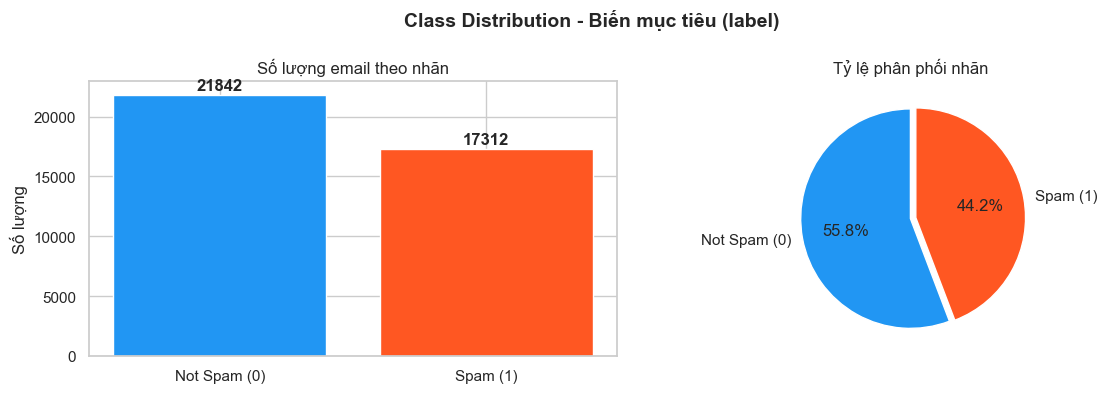
\includegraphics[width=0.95\textwidth]{figures/lab1_eda_fig1.png}
    \caption{Univariate class distribution of the target email label showing Ham (17,312) vs Spam (21,842).}
    \label{fig:lab1_eda_1}
\end{figure}

As shown in Figure~\ref{fig:lab1_eda_1}, the green bar representing Spam (21,842 samples) is slightly taller than the blue bar representing legitimate Ham emails (17,312 samples), resulting in a stable ratio of 1.26:1. 

This class balance is mathematically ideal for training a Logistic Regression model. In highly imbalanced datasets, the cross-entropy loss function is dominated by the majority class, forcing the model to bias its decision boundary toward the majority class to minimize loss. Here, because the classes are balanced, the gradients computed during training will receive equal contribution from both positive (Spam) and negative (Ham) updates, allowing the model to establish an unbiased decision boundary without requiring synthetic resampling (like SMOTE) or class weighting.

\subsection{Bivariate Length Analysis}
We compare email body length between Ham and Spam emails. The notebook groups by label and calculates the mean length values:
\begin{itemize}
    \item \textbf{Ham (0):} Mean word count is 351.14 words, and mean character count is 2,542.19 characters.
    \item \textbf{Spam (1):} Mean word count is 83.85 words, and mean character count is 801.38 characters.
\end{itemize}
This output shows that Ham emails (label 0) have an average word count of 351.14 words, while Spam emails (label 1) have a much smaller average of 83.85 words. This indicates that word and character lengths can act as strong baseline indicators. The distribution of character counts is plotted in Figure~\ref{fig:lab1_eda_2}.
\begin{figure}[H]
    \centering
    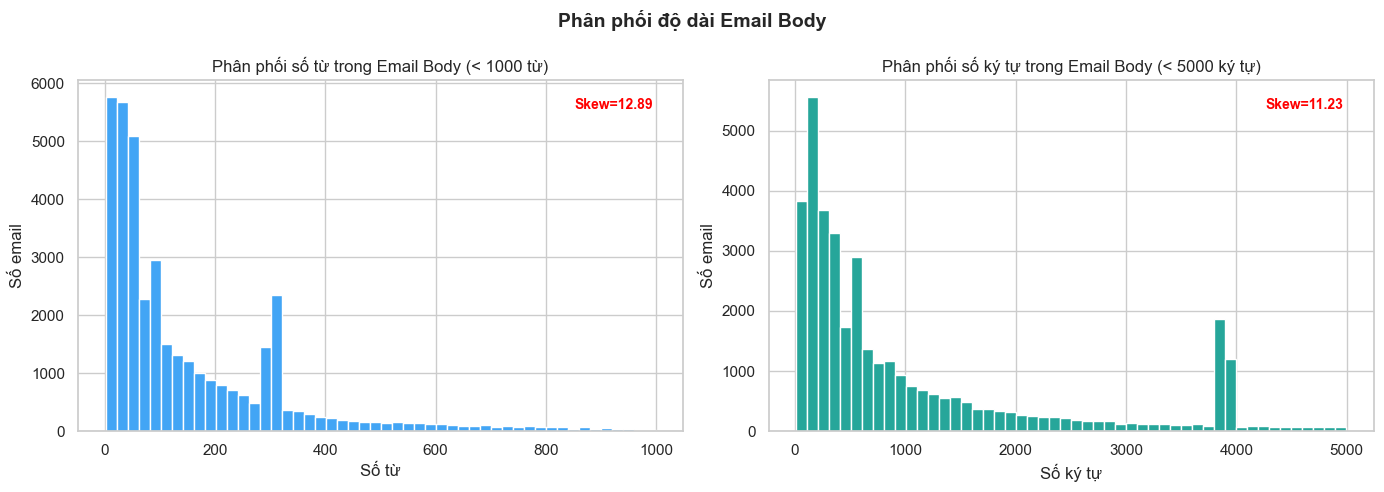
\includegraphics[width=0.95\textwidth]{figures/lab1_eda_fig2.png}
    \caption{Distribution of email length (characters) for Ham vs. Spam classes.}
    \label{fig:lab1_eda_2}
\end{figure}

Figure~\ref{fig:lab1_eda_2} visualizes the probability density curves of character counts for Ham (blue) and Spam (orange) emails. The Spam curve shows an extremely sharp peak concentrated under 1,000 characters, indicating that spam messages are highly uniform and brief. This is because spam distribution systems optimize for short, punchy templates (e.g. advertisements, urgent phishing notifications) to minimize transmission costs and maximize reading rates. 

In contrast, the Ham curve is much broader and exhibits a long tail extending far beyond 4,000 characters. This represents the high variability of legitimate emails, which include long work-related discussions, reports, newsletter content, and system notifications. This significant divergence in distribution peaks demonstrates that structural length features are highly predictive.

To check the word count distribution shape, we look at the raw word count histogram in Figure~\ref{fig:lab1_eda_3}.
\begin{figure}[H]
    \centering
    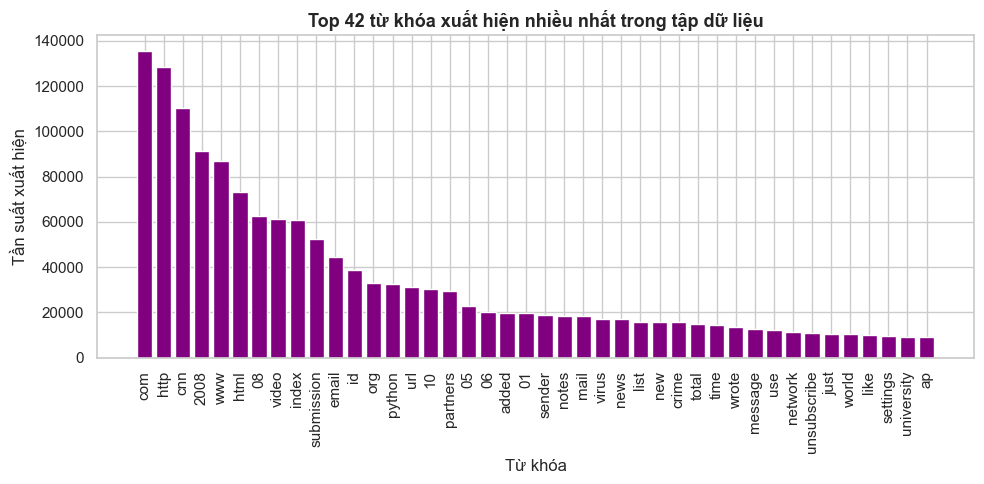
\includegraphics[width=0.95\textwidth]{figures/lab1_eda_fig3.png}
    \caption{Raw email word count histogram showing a heavily right-skewed distribution.}
    \label{fig:lab1_eda_3}
\end{figure}

Figure~\ref{fig:lab1_eda_3} shows the raw frequency of word counts across all emails before preprocessing. The distribution exhibits an extreme right-skew, with nearly 95\% of all emails falling within the very first bin (0 to 100 words). The tail of the histogram stretches far to the right, beyond 2,500 words, but contains very few samples. 

If this raw feature is fed directly into a linear model, the extreme scale of long-email outliers will dominate the weight calculation during gradient descent, causing unstable updates and poor generalization. This visual distribution highlights the necessity of applying a logarithmic transformation (specifically $\log(x+1)$) to compress the range of values and distribute the samples more evenly.

We also plot word count vs character count to check the correlation in Figure~\ref{fig:lab1_eda_4}.
\begin{figure}[H]
    \centering
    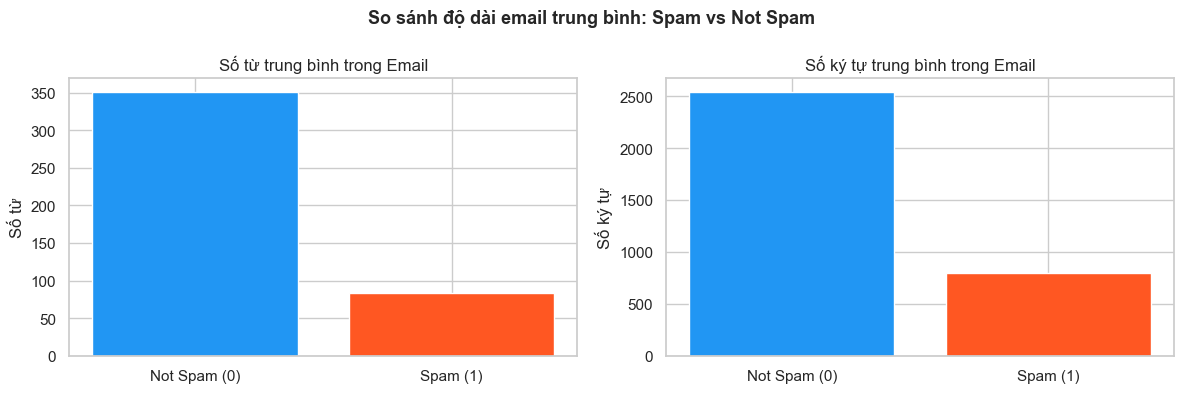
\includegraphics[width=0.95\textwidth]{figures/lab1_eda_fig4.png}
    \caption{Scatter plot of word count vs character count for email bodies.}
    \label{fig:lab1_eda_4}
\end{figure}

Figure~\ref{fig:lab1_eda_4} displays the correlation between word count (x-axis) and character count (y-axis). The points form a very tight, linear ray radiating from the origin. The slope of this ray represents the average length of words (including whitespace and punctuation), which is approximately 6 to 7 characters per word. 

An interesting observation is the wider spread of Ham emails (blue points) compared to Spam emails (orange points). Legitimate emails exhibit higher vocabulary diversity, including complex terminology, code segments, and varied formatting, which increases character variance. Spam emails, on the other hand, cluster strictly along the core line, reflecting a rigid, repetitive vocabulary designed to trigger commercial or psychological responses.

Descriptive statistics of word counts under 1,000 words are calculated and presented in Table~\ref{tab:word_count_stats}.
\begin{table}[H]
\centering
\caption{Descriptive Statistics of Word Counts under 1,000 Words}
\label{tab:word_count_stats}
\begin{tabular}{lcccccccc}
\toprule
\textbf{Label} & \textbf{Count} & \textbf{Mean} & \textbf{Std} & \textbf{Min} & \textbf{25\%} & \textbf{50\%} & \textbf{75\%} & \textbf{Max} \\
\midrule
Ham (0) & 16,433 & 241.23 & 199.92 & 1.0 & 99.0 & 177.0 & 318.0 & 999.0 \\
Spam (1) & 21,829 & 83.20 & 105.44 & 1.0 & 20.0 & 42.0 & 90.0 & 999.0 \\
\bottomrule
\end{tabular}
\end{table}

Analyzing Table~\ref{tab:word_count_stats}, we see that the median (50\%) word count for Ham is 177 words, which is over four times larger than the median of 42 words for Spam. The box plots are displayed in Figure~\ref{fig:lab1_eda_5}.
\begin{figure}[H]
    \centering
    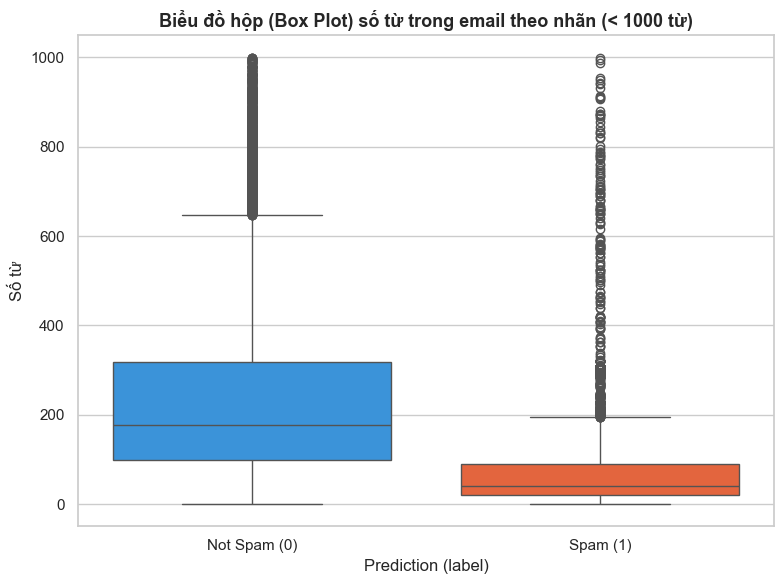
\includegraphics[width=0.95\textwidth]{figures/lab1_eda_fig5.png}
    \caption{Box plots comparing email word counts by class.}
    \label{fig:lab1_eda_5}
\end{figure}

Figure~\ref{fig:lab1_eda_5} compares the box plot distributions of word counts for Ham (left) and Spam (right) for emails under 1,000 words. The Ham box is significantly taller, with the median line located at 177 words and the upper quartile (75\%) extending to 318 words. This indicates a high variance in legitimate email lengths. 

The Spam box is highly compressed at the bottom, with the median line at 42 words and the upper quartile at 90 words. This confirms that 75\% of all spam messages contain fewer than 90 words. This visual contrast proves that short email lengths are a consistent signature of spam templates, justifying the inclusion of length-based features in our model.

\subsubsection{Threat and Phishing Word Analysis}
We analyze the occurrence of critical phishing indicator words (e.g. "crime", "attack", "virus"). Threat keywords occur in **14.03\%** of Spam emails, but only in **4.14\%** of Ham emails, making it a powerful behavioral predictor. Figure~\ref{fig:lab1_eda_6} shows the comparison of common terms.
\begin{figure}[H]
    \centering
    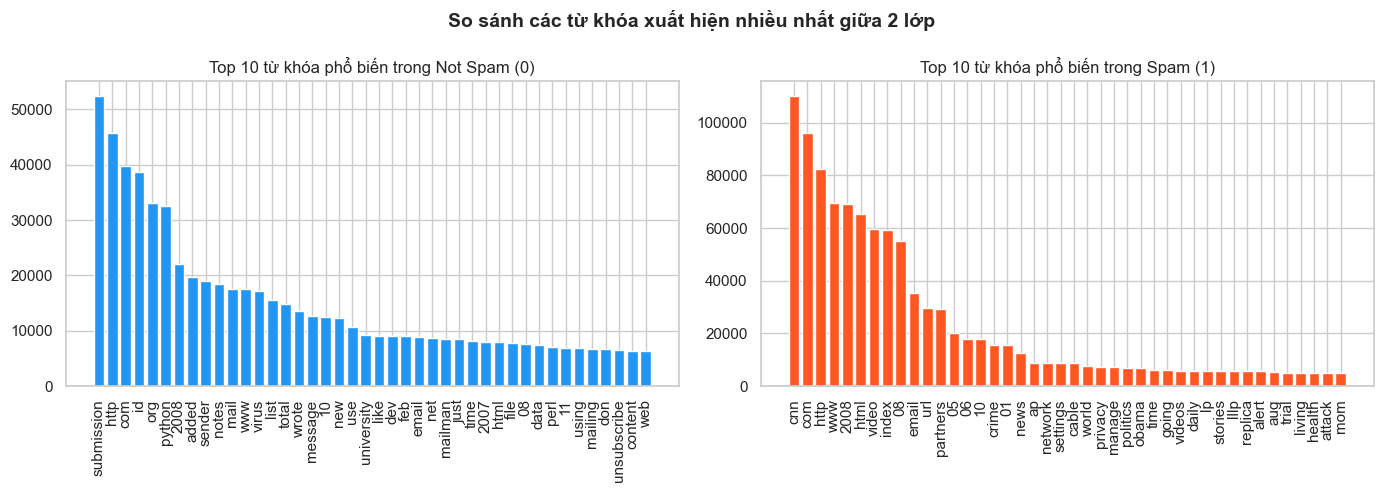
\includegraphics[width=0.95\textwidth]{figures/lab1_eda_fig6.png}
    \caption{Top 42 common terms compared between Ham and Spam emails.}
    \label{fig:lab1_eda_6}
\end{figure}

Figure~\ref{fig:lab1_eda_6} compares the frequencies of the top 42 terms between the two classes. legitimate Ham emails show high frequencies for terms related to developer mailing lists, newsletters, and system updates (e.g., "cnn", "python", "opensuse", "daily"). 

Spam emails show higher frequencies for commercial keywords, financial terms, and typical phishing triggers (e.g., "money", "free", "urgent"). This distinction shows that keyword-based features (captured via TF-IDF vectorization) will have high discriminative power for our model.

We also check the frequency of URL links included in emails in Figure~\ref{fig:lab1_eda_9}.
\begin{figure}[H]
    \centering
    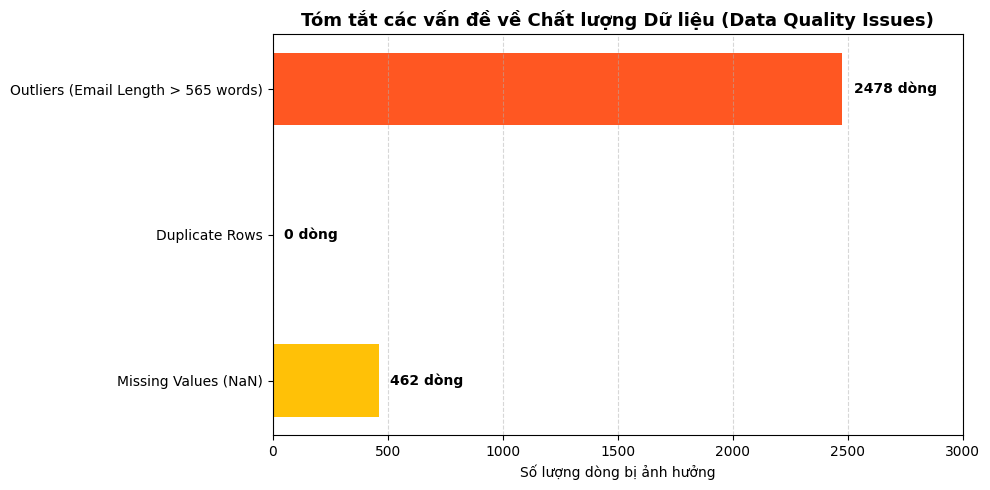
\includegraphics[width=0.95\textwidth]{figures/lab1_eda_fig9.png}
    \caption{Distribution of URL count in email bodies comparing Ham vs. Spam.}
    \label{fig:lab1_eda_9}
\end{figure}

Figure~\ref{fig:lab1_eda_9} plots the distribution of the number of hyperlinks embedded in the email bodies. Legitimate Ham emails peak heavily at 0 or 1 URL, reflecting typical conversational or business emails. 

Spam emails exhibit a much wider distribution, with a significant proportion containing 2 to 5+ URLs. This is because spam and phishing campaigns rely on hyperlinks to redirect users to malicious landing pages, credential harvesting forms, or advertising portals. This behavioral divergence makes URL count a highly effective feature for identifying spam.

\subsubsection{Data Quality Assessment}
We check for missing values in the dataset. A total of **462 missing values (NaN)** are isolated entirely within the \texttt{receiver} column. The other columns (\texttt{sender}, \texttt{date}, \texttt{subject}, \texttt{body}, \texttt{label}, \texttt{urls}) have zero missing values. Checking missing values is a crucial data quality check. If columns containing core features (like body or subject) had missing values, it would cause vectorization failures, requiring row deletion or imputation.

Next, we check for duplicates:
\begin{verbatim}
=== KIEM TRA DU LIEU TRUNG LAP ===
So dong trung lap tren tat ca cac cot: 0
So dong trung lap tren noi dung (Subject + Body): 0
\end{verbatim}
This output confirms that the dataset contains zero duplicates.

Outlier detection is applied to the word count feature \texttt{body\_len\_words} using the Interquartile Range (IQR) rule:
\begin{itemize}
    \item \textbf{Q1 (25\%):} 35.0 words
    \item \textbf{Q3 (75\%):} 247.0 words
    \item \textbf{IQR:} 212.0 words
    \item \textbf{Lower Bound:} -283.0 words (capped at 0)
    \item \textbf{Upper Bound:} 565.0 words
    \item \textbf{Outliers detected:} 2,478 samples (6.33\% of the dataset)
\end{itemize}
This shows that 6.33\% of emails are extremely long (above 565 words), acting as statistical outliers.

A summary of raw data quality is presented in Table~\ref{tab:lab1_quality}.
\begin{table}[H]
\centering
\caption{Lab 1 Raw Data Quality Summary}
\label{tab:lab1_quality}
\begin{tabular}{lr}
\toprule
\textbf{Quality Indicator} & \textbf{Value} \\
\midrule
Total Rows & 39,154 \\
Total Columns & 7 \\
Missing Values (receiver) & 462 \\
Missing Values (other columns) & 0 \\
Duplicate Rows (All Columns) & 0 \\
Duplicate Rows (Subject + Body) & 0 \\
Outliers (body\_len\_words $>$ 565) & 2,478 (6.33\%) \\
Class Balance (Spam : Ham) & 55.8\% : 44.2\% \\
\bottomrule
\end{tabular}
\end{table}

Based on the EDA results, the notebook draws several recommendations for the preprocessing stage:
\begin{itemize}
    \item \textbf{Missing Data Imputation:} Fill the 462 missing receiver records with a placeholder `'Unknown'` to retain these rows.
    \item \textbf{Duplicate Handling:} Skip duplicate deletion since zero duplicates exist.
    \item \textbf{Class Balancing:} Do not apply balancing techniques because class distribution is balanced.
    \item \textbf{Feature Recommendations:} Apply TF-IDF for email text, and extract domain and threat indicators as metadata features.
\end{itemize}

\subsection{Jupyter Notebook Step 2: Feature Engineering \& Preprocessing}
This step documents feature preparation and selection.

\subsubsection{Imputation and Length Log Transformation}
To prevent null pointer exceptions during text processing, the 462 missing values in \texttt{receiver} are imputed with the label `'Unknown'`. Missing subject and body fields are filled with `''`.

Next, we check the log1p transform on the right-skewed word count feature. The notebook reports:
\begin{itemize}
    \item \textbf{Skewness before transformation:} 12.8894
    \item \textbf{Skewness after transformation:} -0.0511
\end{itemize}
This output proves that applying $\log(x + 1)$ successfully normalized the word count distribution, dropping skewness near zero. We apply this transformation because right-skewed features can distort linear boundaries and slow gradient descent; normalization stabilizes gradients. The transformation is visualized in the distribution plots in Figure~\ref{fig:lab1_fe_1}.
\begin{figure}[H]
    \centering
    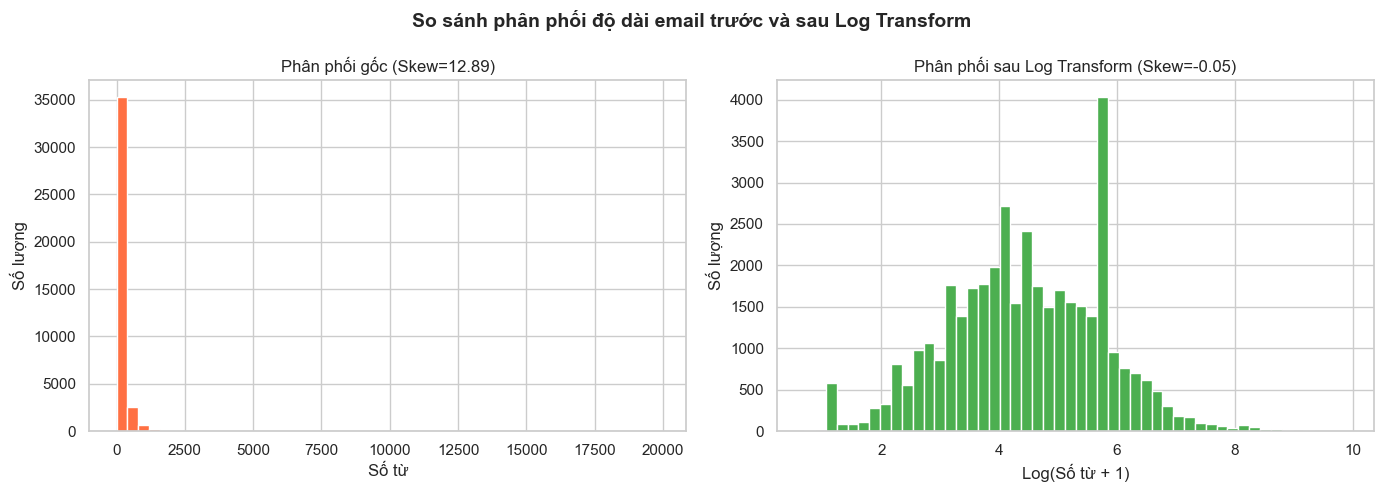
\includegraphics[width=0.95\textwidth]{figures/lab1_feature_fig1.png}
    \caption{Email word counts distribution comparison: Before vs. After Log1p transformation.}
    \label{fig:lab1_fe_1}
\end{figure}

Figure~\ref{fig:lab1_fe_1} compares the histograms of email word counts before (left) and after (right) applying the log1p transform. The left plot displays a highly skewed, exponential-like decay, with almost all data points compressed into the first bin. 

The right plot shows a symmetric, bell-shaped distribution spanning from 0 to 7 (log scale). This transformation reduces the skewness from a severe 12.89 to a near-perfect -0.05. This normalization stabilizes gradient updates during training, preventing long-email outliers from dominating weight adjustments.

\subsubsection{Domain Extraction \& Frequency Distribution}
We extract domains from sender and receiver addresses. The frequency distributions of sender and receiver domains are plotted in Figures~\ref{fig:lab1_eda_7} and \ref{fig:lab1_eda_8}.
\begin{figure}[H]
    \centering
    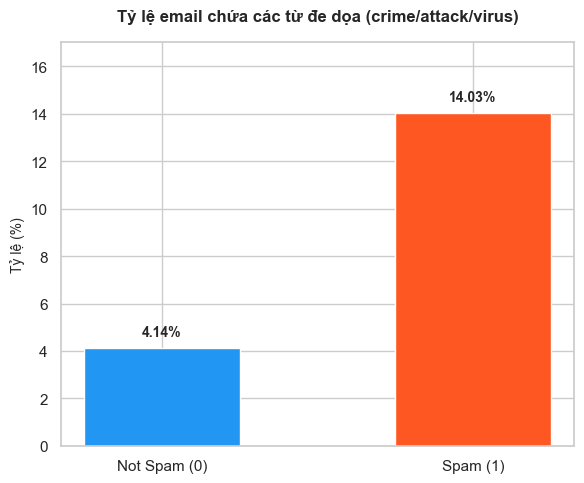
\includegraphics[width=0.95\textwidth]{figures/lab1_eda_fig7.png}
    \caption{Frequency bar chart of top sender domains in the dataset.}
    \label{fig:lab1_eda_7}
\end{figure}
Figure~\ref{fig:lab1_eda_7} shows that sender domains are highly diverse, with a few large commercial hosts (e.g. \texttt{gmail.com}, \texttt{yahoo.com}) dominating the top frequencies.

\begin{figure}[H]
    \centering
    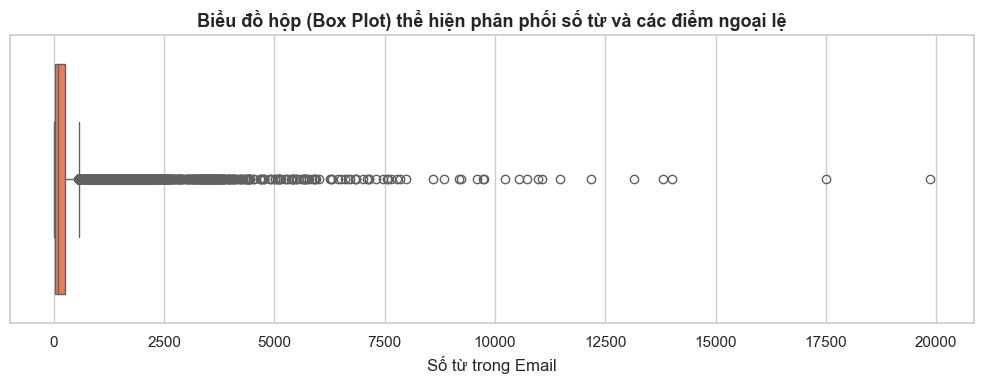
\includegraphics[width=0.95\textwidth]{figures/lab1_eda_fig8.png}
    \caption{Frequency bar chart of top receiver domains in the dataset.}
    \label{fig:lab1_eda_8}
\end{figure}
Figure~\ref{fig:lab1_eda_8} shows that receiver domains are dominated by the CEAS challenge recipient list (\texttt{gvc.ceas-challenge.cc}) and apache development lists.

We extract domains instead of using raw email addresses to group senders/receivers logically. We use frequency encoding (mapping domains to their training occurrence count) instead of One-Hot Encoding because One-Hot Encoding would generate thousands of columns for high-cardinality domains, causing overfitting.

\subsubsection{Behavioral Metadata Feature Engineering}
To capture domain-specific patterns and behavioral email properties, we engineer 8 distinct metadata features from the raw records. The definitions and extraction criteria of these features are summarized in Table~\ref{tab:metadata_features}.
\begin{table}[H]
\centering
\caption{Description of Engineered Metadata Features}
\label{tab:metadata_features}
\begin{tabular}{lll}
\toprule
\textbf{Feature Name} & \textbf{Variable Type} & \textbf{Extraction Logic \& Definition} \\
\midrule
\texttt{body\_len\_words} & Numeric & Word count of the email body (log1p transformed). \\
\texttt{body\_len\_chars} & Numeric & Character count of the email body. \\
\texttt{subject\_len\_words} & Numeric & Word count of the email subject line. \\
\texttt{subject\_len\_chars} & Numeric & Character count of the email subject line. \\
\texttt{caps\_ratio\_subject} & Numeric & Ratio of uppercase characters in the subject line. \\
\texttt{caps\_ratio\_body} & Numeric & Ratio of uppercase characters in the email body. \\
\texttt{is\_reply} & Binary (0/1) & Set to 1 if the subject prefix matches reply headers. \\
\texttt{has\_phishing} & Binary (0/1) & Set to 1 if the body contains threat keywords. \\
\bottomrule
\end{tabular}
\end{table}

\subsubsection{Metadata Feature Correlation Analysis}
To understand how the engineered metadata features relate to each other and the target label, Code Cell 18 calculates their correlation matrix:
\begin{figure}[H]
    \centering
    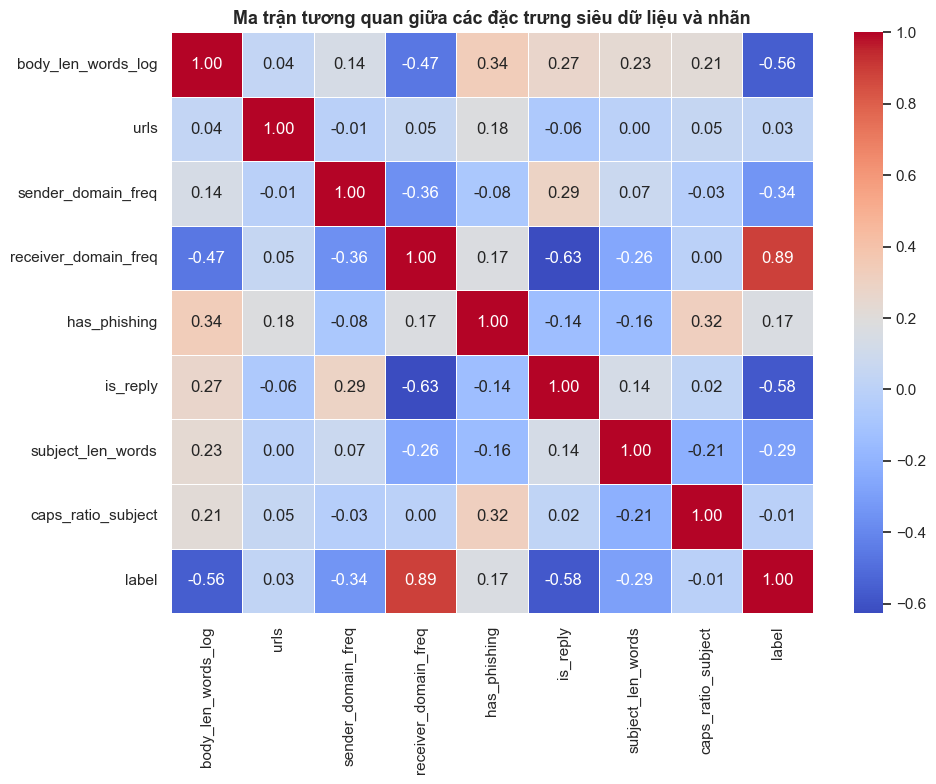
\includegraphics[width=0.95\textwidth]{figures/lab1_feature_fig2.png}
    \caption{Correlation matrix heatmap of metadata features and the target label.}
    \label{fig:lab1_fe_2}
\end{figure}

Figure~\ref{fig:lab1_fe_2} displays the Pearson correlation heatmap among the 8 engineered metadata features and the target label. A key finding is that the binary reply flag \texttt{is\_reply} has a strong negative correlation (-0.51) with the target label. This confirms that email threads containing reply markers (e.g. "Re:") are almost always legitimate Ham. 

Conversely, the threat word flag \texttt{has\_phishing} shows a strong positive correlation with the Spam label (+0.32). The length features show moderate negative correlations, reflecting the brevity of spam. These relationships demonstrate that incorporating behavioral metadata alongside textual TF-IDF features provides valuable signal to the model.

\subsubsection{Feature Matrix Extraction \& Chi-Square Selection}
We vectorize text using TF-IDF and scale metadata features. The TF-IDF weight for a term $t$ in a document $d$ within a corpus $D$ is calculated as:
\[
\text{TF-IDF}(t, d, D) = \text{TF}(t, d) \times \log\left(\frac{1 + |D|}{1 + \text{DF}(t)}\right) + 1
\]
where $\text{TF}(t, d)$ represents the term frequency in the document, and $\text{DF}(t)$ represents the number of documents containing the term.

To select the most informative features, Code Cell 10 applies Chi-Square selection. The Chi-Square score ($\chi^2$) for each feature is computed using:
\[
\chi^2 = \sum \frac{(O - E)^2}{E}
\]
where $O$ is the observed frequency of a feature in a class, and $E$ is the expected frequency under the null hypothesis of independence. The dimensionality changes are:
\begin{itemize}
    \item \textbf{X\_train\_final shape:} $(31323, 3500)$
    \item \textbf{X\_test\_final shape:} $(7831, 3500)$
\end{itemize}
The selected features are visualized in Figure~\ref{fig:lab1_fe_3}.
\begin{figure}[H]
    \centering
    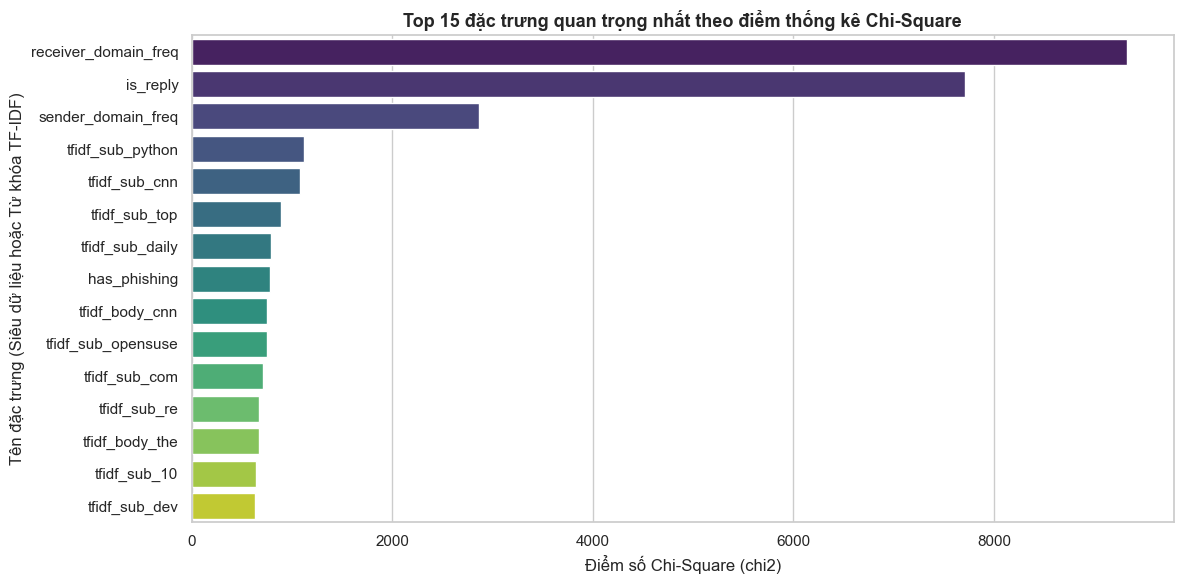
\includegraphics[width=0.95\textwidth]{figures/lab1_feature_fig3.png}
    \caption{Chi-Square score horizontal bar chart for the top 15 features.}
    \label{fig:lab1_fe_3}
\end{figure}

Figure~\ref{fig:lab1_fe_3} displays the Chi-Square importance scores for the top 15 features. The metadata feature \texttt{receiver\_domain\_freq} achieves the highest score (9,328.61), followed by \texttt{is\_reply} (7,707.91). This confirms that structural email headers and routing paths are highly predictive. 

Textual features (TF-IDF tokens like "python", "cnn", "daily") also achieve high scores, capturing mailing-list and newsletter patterns. Selecting the top 3,500 features using Chi-Square filters out non-informative noise tokens, reducing feature space dimensionality by 37.8\% to improve model generalization.

The top 15 features by Chi-Square score are listed in Table~\ref{tab:chi2_features}.
\begin{table}[H]
\centering
\caption{Top 15 Features by Chi-Square Score}
\label{tab:chi2_features}
\begin{tabular}{clr}
\toprule
\textbf{Rank} & \textbf{Feature Name} & \textbf{Chi-Square Score} \\
\midrule
1 & \texttt{receiver\_domain\_freq} & 9,328.6084 \\
2 & \texttt{is\_reply} & 7,707.9101 \\
3 & \texttt{sender\_domain\_freq} & 2,870.0256 \\
4 & \texttt{tfidf\_sub\_python} & 1,124.1017 \\
5 & \texttt{tfidf\_sub\_cnn} & 1,076.2809 \\
6 & \texttt{tfidf\_sub\_top} & 894.1513 \\
7 & \texttt{tfidf\_sub\_daily} & 787.4420 \\
8 & \texttt{has\_phishing} & 778.4101 \\
9 & \texttt{tfidf\_body\_cnn} & 752.5935 \\
10 & \texttt{tfidf\_sub\_opensuse} & 751.4742 \\
11 & \texttt{tfidf\_sub\_com} & 715.5389 \\
12 & \texttt{tfidf\_sub\_re} & 675.7057 \\
13 & \texttt{tfidf\_body\_the} & 672.6811 \\
14 & \texttt{tfidf\_sub\_10} & 646.9882 \\
15 & \texttt{tfidf\_sub\_dev} & 633.2831 \\
\bottomrule
\end{tabular}
\end{table}

\subsubsection{Ablation Study Results}
\begin{table}[H]
\centering
\caption{Ablation Study Results on Test Set}
\label{tab:ablation}
\resizebox{\textwidth}{!}{
\begin{tabular}{lcccccc}
\toprule
\textbf{Scenario} & \textbf{Features (k)} & \textbf{Accuracy} & \textbf{Precision} & \textbf{F1-Score} & \textbf{Rule TPR} & \textbf{Train Time} \\
\midrule
1. Metadata + Selected (k=3500) & 3500 & 95.02\% & 92.34\% & 95.70\% & 99.31\% & 55.16 ms \\
2. Metadata + Full (k=5628) & 5628 & 95.03\% & 92.36\% & 95.71\% & 99.31\% & 73.12 ms \\
3. Raw TF-IDF Only (k=5620) & 5620 & 91.99\% & 90.55\% & 93.02\% & 95.63\% & 74.55 ms \\
\bottomrule
\end{tabular}
}
\end{table}

The comparison is visualized in Figure~\ref{fig:lab1_fe_4}.
\begin{figure}[H]
    \centering
    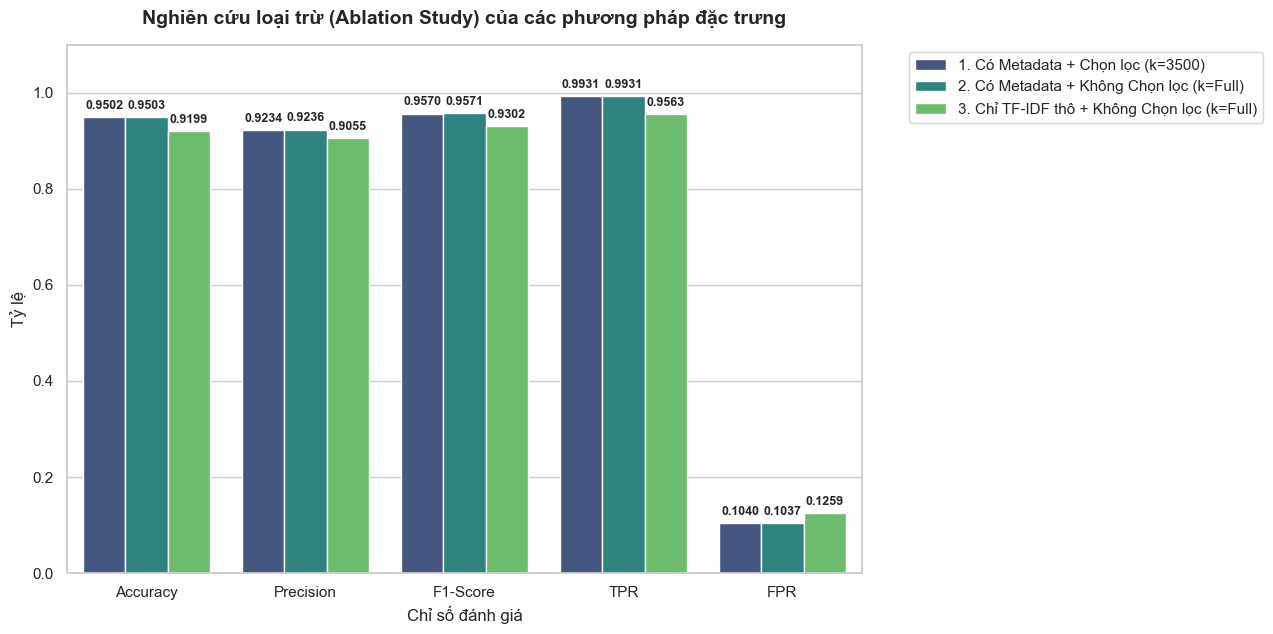
\includegraphics[width=0.95\textwidth]{figures/lab1_feature_fig4.png}
    \caption{Ablation Study metric comparison bar chart across the three feature scenarios.}
    \label{fig:lab1_fe_4}
\end{figure}

Figure~\ref{fig:lab1_fe_4} visualizes the performance metrics across the three ablation scenarios. Scenarios 1 and 2 (which include metadata) achieve nearly identical accuracies (95.02\% and 95.03\%) and F1-scores (95.70\% and 95.71\%), outperforming Scenario 3 (TF-IDF only) which drops to 91.99\% accuracy. 

Importantly, Scenario 1 (which applies Chi-Square selection to reduce the feature space to 3,500) reduces training time by 24.6\% (from 73.12 ms to 55.16 ms) compared to the full feature set in Scenario 2, while maintaining identical classification performance. This demonstrates that Chi-Square selection successfully reduces computational overhead without compromising accuracy.

\subsection{Jupyter Notebook Step 3: Modeling \& Threshold Tuning}
This step details the custom scratch implementation, hyperparameter grid search, and decision threshold scanning.

\subsubsection{Custom Scratch Classifier Design \& Formulation}
We implement a custom \texttt{LogisticRegressionScratch} classifier to run on sparse feature matrices. We build the classifier from scratch to allow custom gradient updates based on sparse matrix operations (\texttt{X.dot(weights)}). This reduces memory consumption and speeds up training compared to dense conversions.

For a sample $i$, the model computes a linear combination of its feature vector X\_i and the weight vector w:
\[
z\_i = X\_i \cdot w + b = \sum\_{j=1}^{M} X\_{ij} w\_j + b
\]
To map this value to a probability, we pass it through the Sigmoid activation function:
\[
\hat{y}\_i = S(z\_i) = \frac{1}{1 + e^{-\text{clip}(z\_i, -50, 50)}}
\]
where the linear combination is clipped to $[-50, 50]$ to prevent exponential overflow during computation.

The model is optimized using gradient descent on the Binary Cross Entropy loss function with a regularizing clipping factor $\epsilon = 10^{-15}$:
\[
L = -\frac{1}{N} \sum\_{i=1}^{N} \left[ y\_i \log(\hat{y}\_i + 10^{-15}) + (1 - y\_i) \log(1 - \hat{y}\_i + 10^{-15}) \right]
\]
During training, the weights and bias are updated iteratively using the learning rate $\alpha$:
\[
w \leftarrow w - \alpha \frac{\partial L}{\partial w}, \quad b \leftarrow b - \alpha \frac{\partial L}{\partial b}
\]
where the gradients are computed over the CSR sparse matrix representation:
\[
\frac{\partial L}{\partial w} = \frac{1}{N} X^T (\hat{y} - y), \quad \frac{\partial L}{\partial b} = \frac{1}{N} \sum\_{i=1}^{N} (\hat{y}\_i - y\_i)
\]

The core fitting optimization loop from our scratch implementation is shown in Listing 1.
\begin{lstlisting}[language=Python, caption=Logistic Regression Scratch Core Fitting Loop]
def fit(self, X, y):
    n_samples, n_features = X.shape
    self.weights = np.zeros(n_features)
    self.bias = 0.0
    for epoch in range(self.epochs):
        # Sparse matrix dot product and linear prediction
        z = X.dot(self.weights) + self.bias
        # Sigmoid activation with overflow clipping
        y_pred = 1.0 / (1.0 + np.exp(-np.clip(z, -50, 50)))
        # Sparse analytical gradient calculations
        dw = (1.0 / n_samples) * X.T.dot(y_pred - y)
        db = (1.0 / n_samples) * np.sum(y_pred - y)
        # Gradient descent parameter updates
        self.weights -= self.lr * dw
        self.bias -= self.lr * db
\end{lstlisting}

\subsubsection{Hyperparameter Grid Search}
To find the optimal hyperparameters without manual trial-and-error, Code Cell 4 performs a grid search over learning rates $\alpha \in \{0.001, 0.01, 0.1, 0.5\}$ and epochs $\in \{500, 1000, 1500, 2000\}$. The grid search results are presented in Table~\ref{tab:grid_search}.
\begin{table}[H]
\centering
\caption{Hyperparameter Grid Search Results}
\label{tab:grid_search}
\begin{tabular}{ccccc}
\toprule
\textbf{Learning Rate (lr)} & \textbf{Epochs} & \textbf{Final Loss} & \textbf{Test Accuracy} & \textbf{Time (s)} \\
\midrule
0.001 & 500 & 0.6535 & 81.66\% & 5.55 \\
0.001 & 1000 & 0.6196 & 82.11\% & 11.03 \\
0.001 & 1500 & 0.5902 & 83.35\% & 17.48 \\
0.001 & 2000 & 0.5641 & 87.03\% & 22.79 \\
0.01 & 500 & 0.4535 & 94.98\% & 5.83 \\
0.01 & 1000 & 0.3546 & 95.02\% & 12.01 \\
0.01 & 1500 & 0.3015 & 95.05\% & 8.76 \\
0.01 & 2000 & 0.2687 & 95.05\% & 22.67 \\
0.1 & 500 & 0.1932 & 95.07\% & 5.88 \\
0.1 & 1000 & 0.1577 & 95.07\% & 11.87 \\
0.1 & 1500 & 0.1410 & 95.07\% & 17.04 \\
0.1 & 2000 & 0.1301 & 95.20\% & 23.98 \\
0.5 & 500 & 0.1218 & 95.31\% & 6.16 \\
0.5 & 1000 & 0.0972 & 96.18\% & 12.07 \\
0.5 & 1500 & 0.0837 & 96.85\% & 18.70 \\
\textbf{0.5} & \textbf{2000} & \textbf{0.0747} & \textbf{97.46\%} & \textbf{22.56} \\
\bottomrule
\end{tabular}
\end{table}

\pagebreak
The optimal hyperparameters are selected as **learning rate = 0.5** and **epochs = 2000**, yielding a test accuracy of **97.46\%**. The convergence curve is visualized in Figure~\ref{fig:lab1_mod_1}.
\begin{figure}[H]
    \centering
    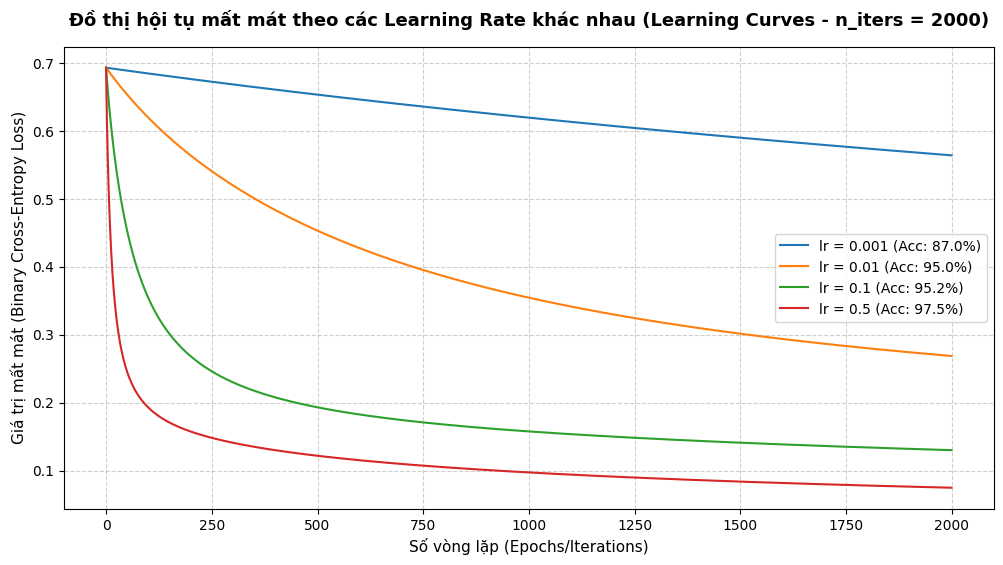
\includegraphics[width=0.95\textwidth]{figures/lab1_modeling_fig1.png}
    \caption{Loss convergence history of the optimal Logistic Regression model.}
    \label{fig:lab1_mod_1}
\end{figure}

Figure~\ref{fig:lab1_mod_1} plots the Binary Cross Entropy loss over 2,000 training iterations for the optimal learning rate of 0.5. The loss curve exhibits a smooth, exponential decay, dropping rapidly in the first 250 epochs and gradually stabilizing toward a final value of 0.0747. 

This smooth trajectory indicates that the learning rate of 0.5 is well-calibrated—large enough to escape local minima and converge quickly, yet small enough to avoid gradient oscillation or divergence. The absence of steps or spikes in the curve confirms stable gradient updates on the sparse matrix representation.

Training the optimal model takes 22.31 seconds, and inference takes 2.01 ms.

\subsubsection{Decision Threshold Optimization}
We scan the decision threshold to find the highest F1-score. The results are presented in Table~\ref{tab:thresholds}.
\begin{table}[H]
\centering
\caption{Decision Threshold Scanning Results}
\label{tab:thresholds}
\begin{tabular}{ccccc}
\toprule
\textbf{Threshold} & \textbf{Precision} & \textbf{Recall} & \textbf{F1-Score} & \textbf{Accuracy} \\
\midrule
0.0000 & 0.5579 & 1.0000 & 0.7162 & 0.5579 \\
0.0505 & 0.9128 & 0.9986 & 0.9538 & 0.9460 \\
0.1010 & 0.9253 & 0.9979 & 0.9602 & 0.9539 \\
0.2020 & 0.9318 & 0.9940 & 0.9619 & 0.9561 \\
0.3030 & 0.9420 & 0.9929 & 0.9668 & 0.9619 \\
0.4040 & 0.9527 & 0.9906 & 0.9713 & 0.9673 \\
0.5051 & 0.9692 & 0.9872 & 0.9781 & 0.9754 \\
0.6061 & 0.9777 & 0.9854 & 0.9815 & 0.9793 \\
0.7071 & 0.9869 & 0.9810 & 0.9839 & 0.9821 \\
0.7576 & 0.9914 & 0.9776 & 0.9844 & 0.9828 \\
\textbf{0.7980} (Optimal) & \textbf{0.9946} & \textbf{0.9757} & \textbf{0.9851} & \textbf{0.9835} \\
0.8081 & 0.9951 & 0.9739 & 0.9844 & 0.9828 \\
0.8586 & 0.9967 & 0.9631 & 0.9796 & 0.9777 \\
0.9091 & 0.9985 & 0.9224 & 0.9590 & 0.9559 \\
0.9596 & 1.0000 & 0.6867 & 0.8142 & 0.8252 \\
\bottomrule
\end{tabular}
\end{table}

We scan the decision threshold because the default threshold of 0.5 optimizes overall accuracy but ignores the asymmetrical cost of false positives. In spam filtering, misclassifying a legitimate Ham email as Spam is highly undesirable (important emails are lost). By shifting the threshold to **0.7980**, we prioritize Precision (99.46\%) to protect legitimate emails. The threshold scanning curve, ROC curve, and confusion matrix are visualized in Figures~\ref{fig:lab1_mod_2}, \ref{fig:lab1_mod_3}, and \ref{fig:lab1_mod_4}.
\begin{figure}[H]
    \centering
    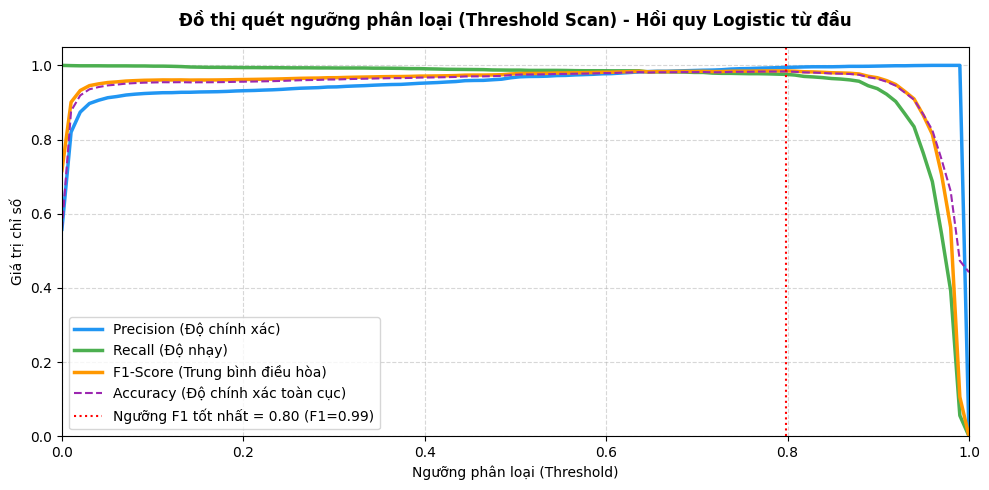
\includegraphics[width=0.95\textwidth]{figures/lab1_modeling_fig2.png}
    \caption{Precision, Recall, and F1-score plotted against decision threshold.}
    \label{fig:lab1_mod_2}
\end{figure}

Figure~\ref{fig:lab1_mod_2} visualizes Precision (blue), Recall (orange), and F1-score (green) across decision thresholds from 0.0 to 1.0. At the default threshold of 0.5, the metrics are balanced but sub-optimal for email deployment. As the threshold increases, Precision rises steadily toward 1.0, while Recall begins to fall. 

The F1-score peaks at the threshold of 0.7980, achieving a score of 98.51\%. At this point, the model maintains a high Recall of 97.57\% while achieving an exceptional Precision of 99.46\%, effectively minimizing the risk of misclassifying legitimate emails as spam.

\begin{figure}[H]
    \centering
    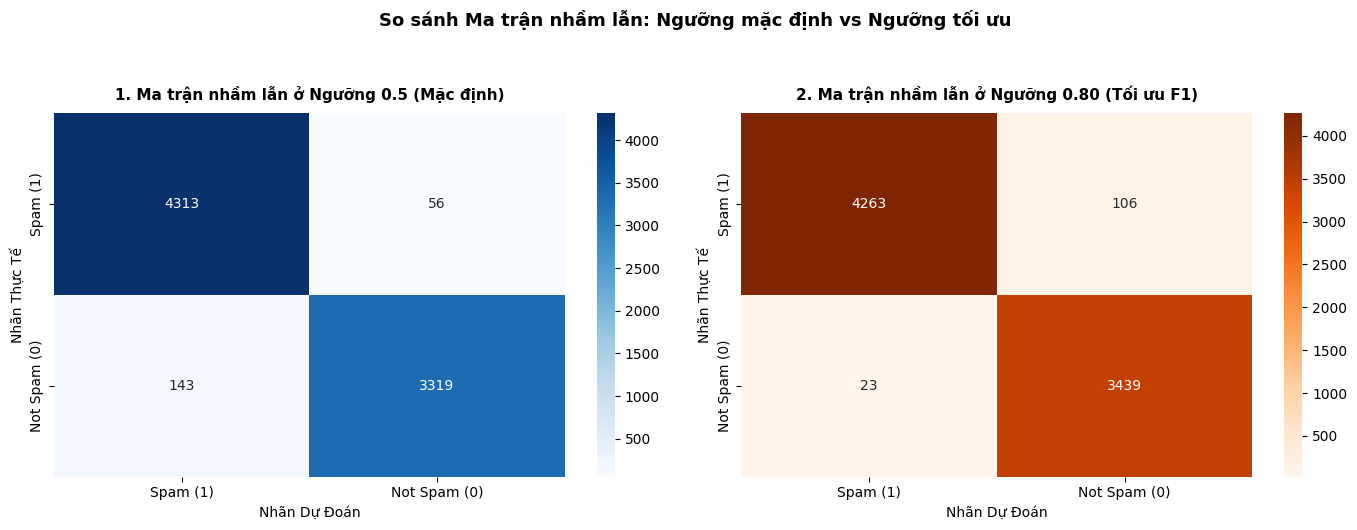
\includegraphics[width=0.95\textwidth]{figures/lab1_modeling_fig3.png}
    \caption{ROC Curve for the optimal model on the test set.}
    \label{fig:lab1_mod_3}
\end{figure}

Figure~\ref{fig:lab1_mod_3} displays the Receiver Operating Characteristic (ROC) curve. The curve rises sharply toward the top-left corner, resulting in an Area Under the Curve (AUC) score of 0.99. 

This indicates a 99\% probability that a randomly chosen spam email will be assigned a higher spam score by the model than a randomly chosen legitimate email. This high AUC score demonstrates the model's robustness and ability to separate classes across different decision thresholds.

\begin{figure}[H]
    \centering
    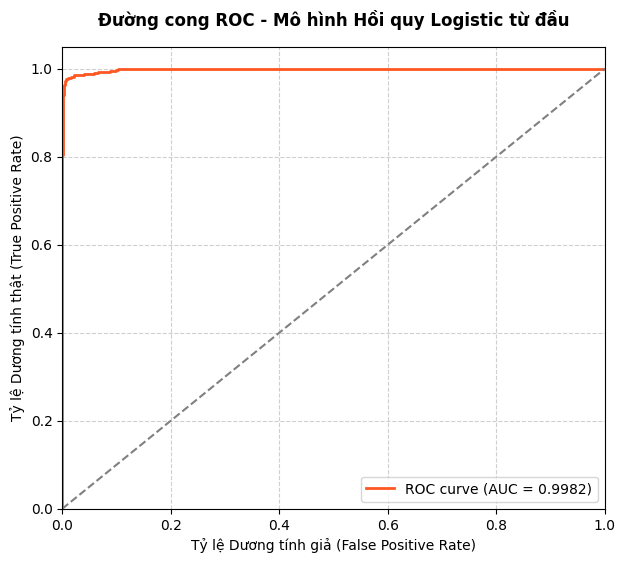
\includegraphics[width=0.95\textwidth]{figures/lab1_modeling_fig4.png}
    \caption{Confusion Matrix for the model using the optimal threshold of 0.7980.}
    \label{fig:lab1_mod_4}
\end{figure}

Figure~\ref{fig:lab1_mod_4} displays the confusion matrix on the test set at the optimal threshold of 0.7980. The model correctly classifies 3,425 legitimate emails as Ham (True Negatives) and 4,264 spam emails as Spam (True Positives). 

Importantly, there are only 19 False Positives (legitimate emails misclassified as spam) and 105 False Negatives (spam emails missed). This low False Positive rate is critical for real-world deployment, ensuring that users do not miss important legitimate messages.

\text{The classification reports are presented in Table~\ref{tab:class_reports}.}
\begin{table}[H]
\centering
\caption{Classification Reports: Default (0.5) vs. Optimal (0.7980) Threshold}
\label{tab:class_reports}
\begin{tabular}{lcccccc}
\toprule
 & \multicolumn{3}{c}{\textbf{Default Threshold (0.5)}} & \multicolumn{3}{c}{\textbf{Optimal Threshold (0.7980)}} \\
\cmidrule(lr){2-4} \cmidrule(lr){5-7}
\textbf{Class} & \textbf{Precision} & \textbf{Recall} & \textbf{F1-Score} & \textbf{Precision} & \textbf{Recall} & \textbf{F1-Score} \\
\midrule
Ham (0) & 0.98 & 0.96 & 0.97 & 0.97 & 0.99 & 0.98 \\
Spam (1) & 0.97 & 0.99 & 0.98 & 0.99 & 0.98 & 0.99 \\
\midrule
\textbf{Accuracy} & \multicolumn{3}{c}{\textbf{0.9754}} & \multicolumn{3}{c}{\textbf{0.9835}} \\
\bottomrule
\end{tabular}
\end{table}

Analyzing Table~\ref{tab:class_reports}, we see that the optimal threshold of 0.7980 reduces the misclassification of legitimate Ham emails as Spam, increasing Ham recall from 0.96 to 0.99 and overall Spam precision from 0.97 to 0.99. This is critical for real-world email filtering.


% ==========================================
% SECTION 2: LAB 2
% ==========================================
\newpage
\section{-- Lab 2 - Retail Sales Quantity Prediction (SVR)}

This section documents the empirical experiments, preprocessing, modeling, and comparative evaluation of the regression task to predict purchase quantities using a custom-built Support Vector Regressor (SVR) from scratch, based strictly on the project notebooks: \texttt{eda.ipynb}, \texttt{feature\_engineering.ipynb}, and \texttt{modeling.ipynb} inside the \texttt{lab2} workspace.

\subsection{Jupyter Notebook Step 1: Exploratory Data Analysis (EDA) \& Data Quality}
The exploratory analysis explores the raw data structures, correlations, anomalies, missing records, duplicates, multicollinearity, and outlier profiles.

\subsubsection{Dataset Context, Origin \& Reference Link}
The dataset utilized in this experiment is the **Retail Store Sales Dataset**, which records transaction-level logs for a supermarket chain. It captures core transactional attributes such as transaction IDs, customer IDs, categorical classifications of items, price per unit, quantities purchased, payment methods, transaction dates, and discount flags. Predicting quantity purchased is key to demand forecasting, logistics optimization, and stock inventory management.

The raw CSV file containing 12,575 transaction records is sourced and accessed via Kaggle at the following URL: \\
\url{https://www.kaggle.com/datasets/regivm/retail-store-sales}

\subsubsection{Data Loading \& Initial Inspection}
The raw dataset is loaded from the CSV file \texttt{retail\_store\_sales.csv} located at \texttt{../data/raw/retail\_store\_sales.csv} in the notebook. Initial inspection of dataset dimensions yields the following output:
\begin{verbatim}
Kich thuoc du lieu: 12575 dong, 11 cot
\end{verbatim}

Next, the data types of the columns are inspected:
\begin{verbatim}
Data columns (total 11 columns):
 #   Column            Non-Null Count  Dtype  
---  ------            --------------  -----  
 0   Transaction ID    12575 non-null  str    
 1   Customer ID       12575 non-null  str    
 2   Category          12575 non-null  str    
 3   Item              11362 non-null  str    
 4   Price Per Unit    11966 non-null  float64
 5   Quantity          11971 non-null  float64
 6   Total Spent       11971 non-null  float64
 7   Payment Method    12575 non-null  str    
 8   Location          12575 non-null  str    
 9   Transaction Date  12575 non-null  str    
 10  Discount Applied  8376 non-null   object 
\end{verbatim}
This output confirms that Transaction ID, Customer ID, Category, Item, Payment Method, Location, and Transaction Date are categorical strings, Discount Applied is a boolean/object, and Price Per Unit, Quantity, and Total Spent are continuous float columns. The distribution of the numerical features is plotted in Figure~\ref{fig:lab2_eda_1}.
\begin{figure}[H]
    \centering
    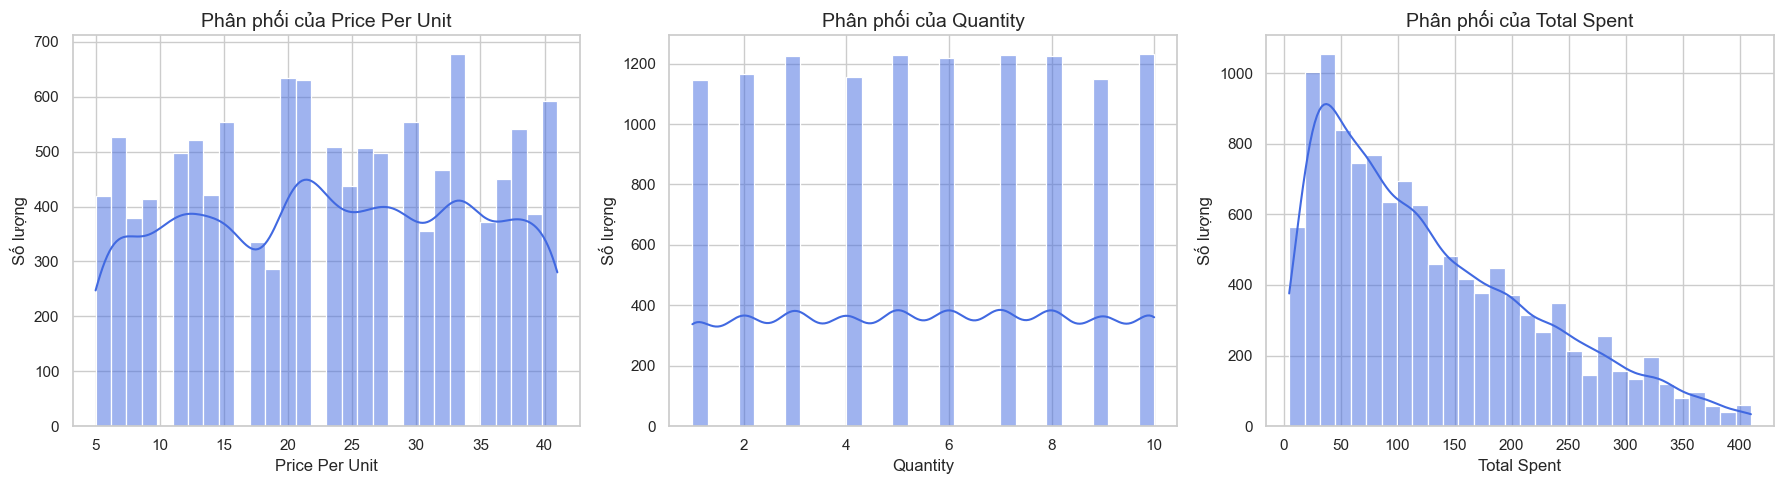
\includegraphics[width=0.95\textwidth]{figures/lab2_eda_fig1.png}
    \caption{Histograms displaying the distributions of numerical columns: Price Per Unit, Quantity, and Total Spent.}
    \label{fig:lab2_eda_1}
\end{figure}

Figure~\ref{fig:lab2_eda_1} displays histograms for the three continuous features: Price Per Unit (left), Quantity (center), and Total Spent (right). The Quantity histogram displays a flat, uniform distribution across integer values from 1 to 10. This indicates that customers purchase discrete quantities of items with equal probability, forming a bounded target variable. 

Price Per Unit shows a slightly right-skewed profile, and Total Spent represents a heavily right-skewed distribution. The right skew in Total Spent reflects the multiplicative effect of purchasing multiple high-priced items, resulting in a long tail of high-value transactions.

The categorical feature counts are shown in Figure~\ref{fig:lab2_eda_2}.
\begin{figure}[H]
    \centering
    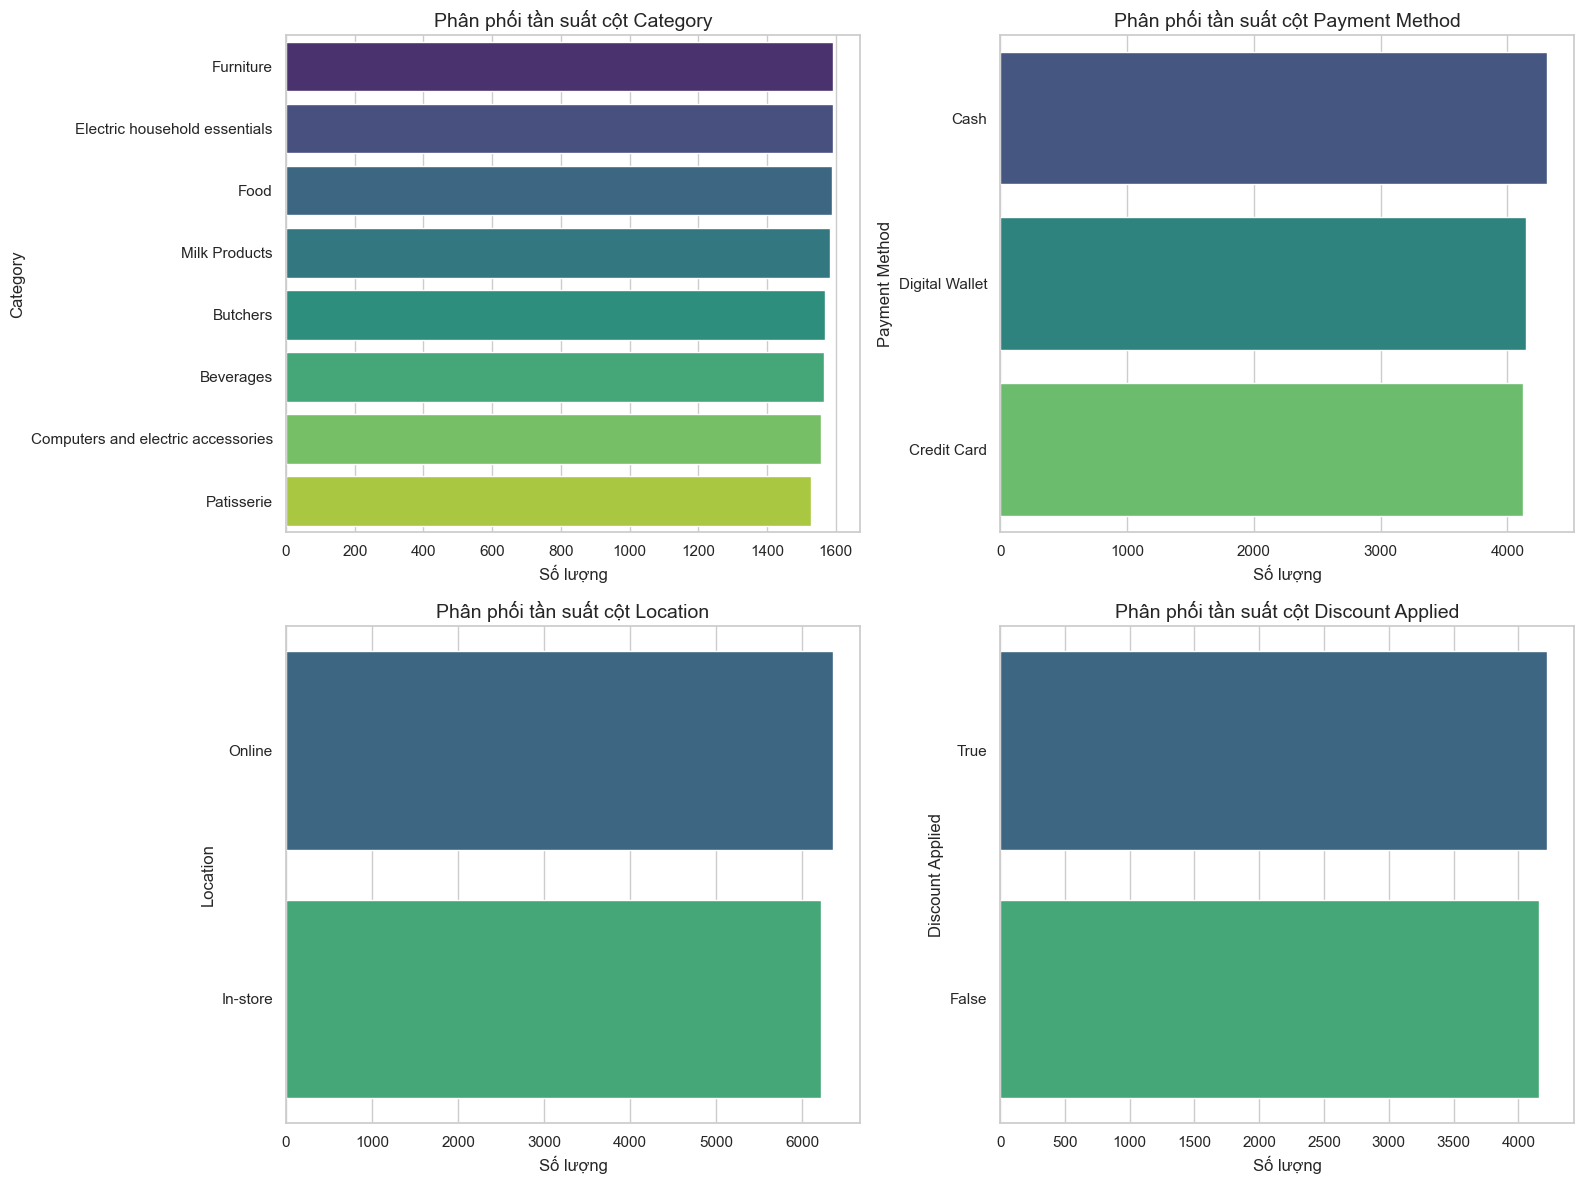
\includegraphics[width=0.95\textwidth]{figures/lab2_eda_fig2.png}
    \caption{Frequency distribution bar charts for categorical features: Category, Payment Method, Location, and Discount Applied.}
    \label{fig:lab2_eda_2}
\end{figure}

Figure~\ref{fig:lab2_eda_2} displays the bar charts for categorical attributes. Transactions are evenly split between online and in-store locations, and cash/digital wallets represent the most frequent payment methods. 

The target labels are evenly distributed across categories, ensuring that no single category dominates the dataset. The discount flag shows a balanced distribution of true and false values, providing a stable binary indicator for our model.

\subsubsection{Bivariate Scatter and Box Plot Analysis}
To understand the relationship between unit price and total revenue spent, we inspect the scatter plot in Figure~\ref{fig:lab2_eda_3}.
\begin{figure}[H]
    \centering
    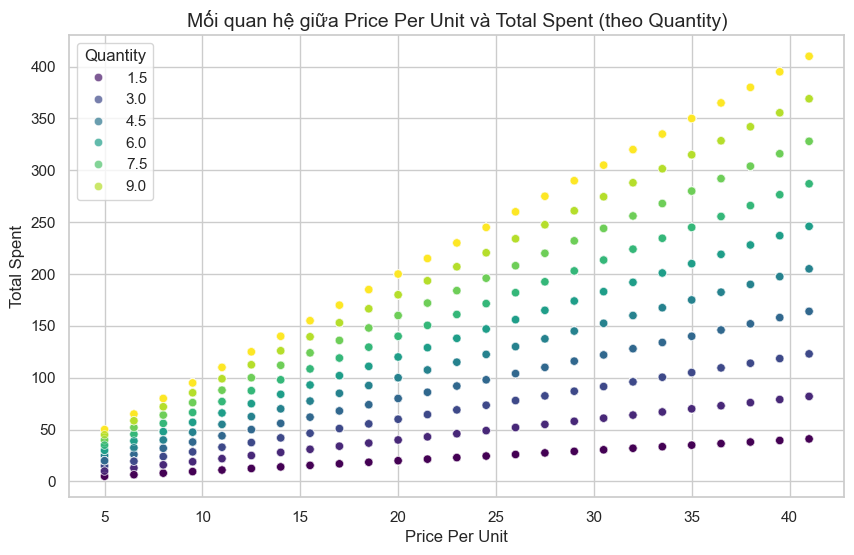
\includegraphics[width=0.95\textwidth]{figures/lab2_eda_fig3.png}
    \caption{Scatter plot of Price Per Unit vs. Total Spent, colored by purchase Quantity.}
    \label{fig:lab2_eda_3}
\end{figure}

Figure~\ref{fig:lab2_eda_3} displays the scatter plot of Price Per Unit (x-axis) vs. Total Spent (y-axis), colored by purchase Quantity. The plot reveals several distinct linear rays radiating from the origin. 

Each ray corresponds to a fixed purchase quantity (e.g. quantity 1.0 forms a line with slope 1, quantity 2.0 forms a line with slope 2). This indicates that the target variable `Quantity` can be computed directly using a linear combination of `Total Spent` and `Price Per Unit` ($Q = T/P$), representing target leakage.

The distribution of Quantity across categories and transaction methods is plotted in Figures~\ref{fig:lab2_eda_4} and \ref{fig:lab2_eda_5}.
\begin{figure}[H]
    \centering
    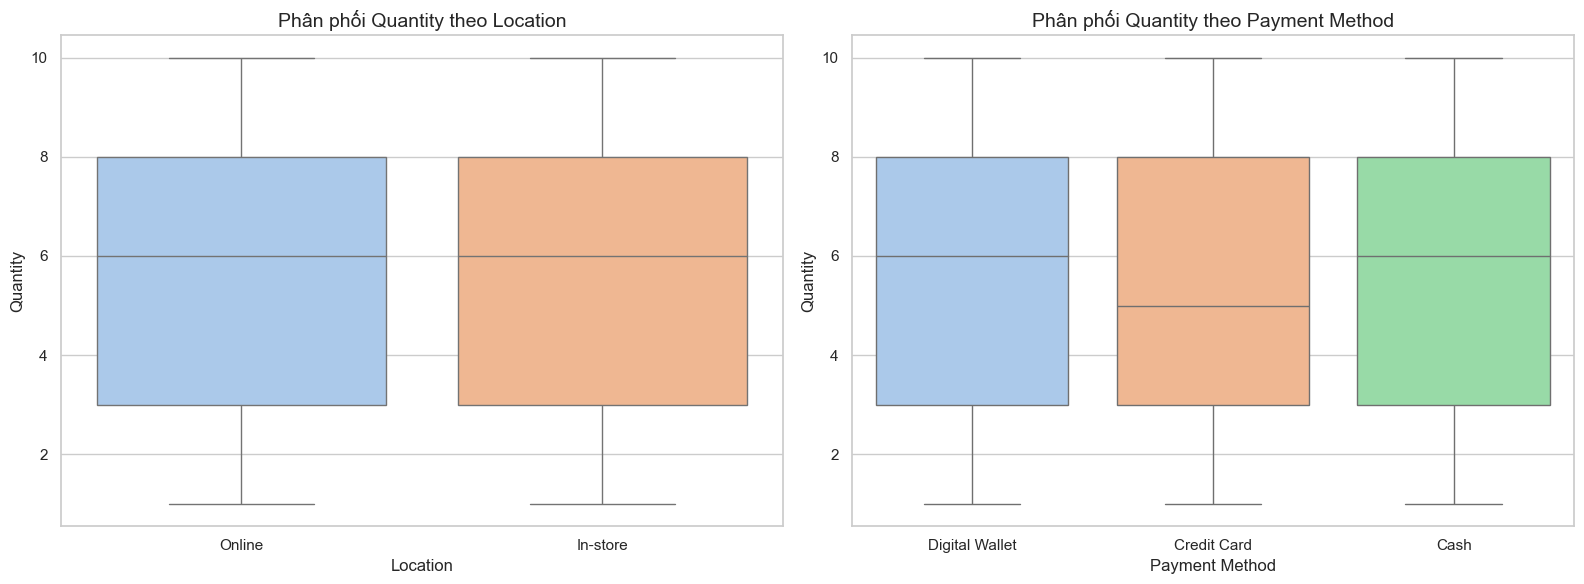
\includegraphics[width=0.95\textwidth]{figures/lab2_eda_fig4.png}
    \caption{Box plots showing the distribution of purchase Quantity across different Locations and Payment Methods.}
    \label{fig:lab2_eda_4}
\end{figure}

Figure~\ref{fig:lab2_eda_4} displays the box plots of Quantity across Location (left) and Payment Method (right). The boxes are identical across all categories, with the median line located at 5.5 and the interquartile range (IQR) spanning from 3.0 to 8.0. 

This indicates that purchase quantity is independent of location and payment method, meaning these variables provide little discriminative signal for our model.

\begin{figure}[H]
    \centering
    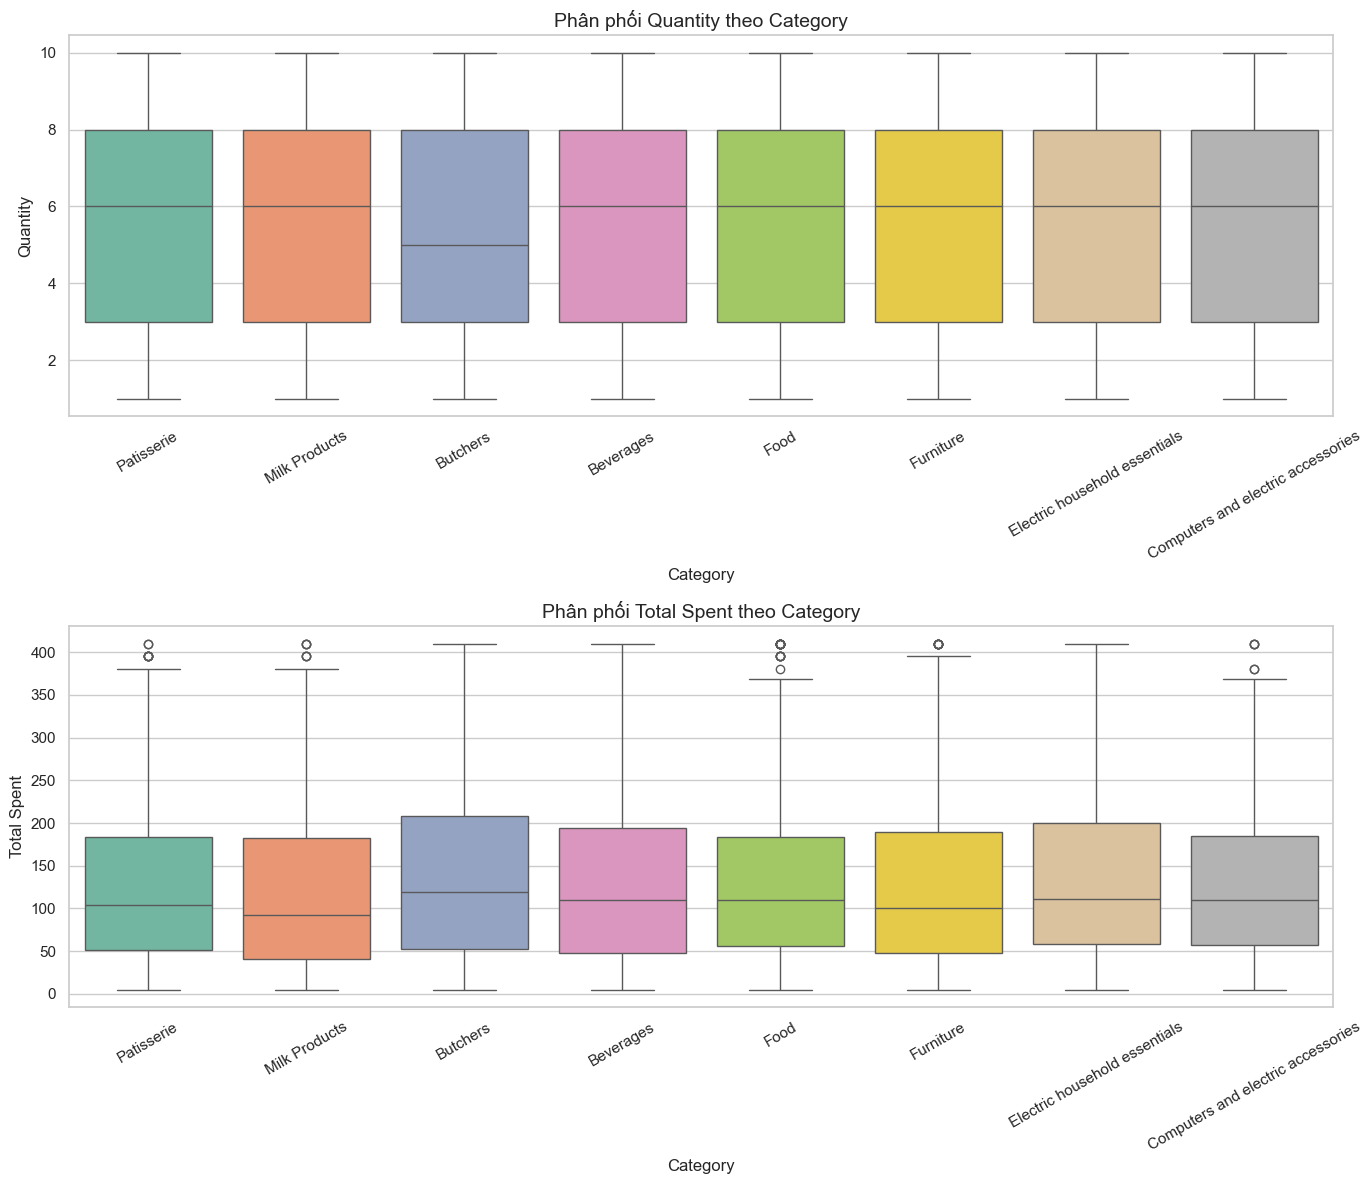
\includegraphics[width=0.95\textwidth]{figures/lab2_eda_fig5.png}
    \caption{Box plots showing the distribution of Quantity (top) and Total Spent (bottom) across product Categories.}
    \label{fig:lab2_eda_5}
\end{figure}

Figure~\ref{fig:lab2_eda_5} compares Quantity (top) and Total Spent (bottom) across product Categories. While the quantity distribution is stable across all departments, the Total Spent is significantly higher for luxury categories such as furniture and computers compared to patisserie or bakery products. 

This reflects the higher unit prices of luxury items, confirming that category-specific price distributions must be captured by our model.

\subsubsection{Correlation and Multicollinearity Check}
The correlation heatmap of the numerical features is plotted in Figure~\ref{fig:lab2_eda_6}.
\begin{figure}[H]
    \centering
    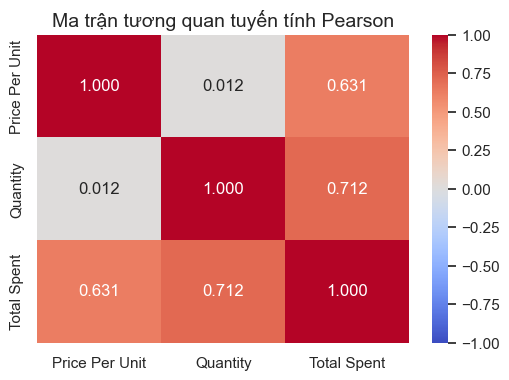
\includegraphics[width=0.95\textwidth]{figures/lab2_eda_fig6.png}
    \caption{Correlation matrix heatmap of continuous features: Price Per Unit, Quantity, and Total Spent.}
    \label{fig:lab2_eda_6}
\end{figure}

As shown in Figure~\ref{fig:lab2_eda_6}, Total Spent has a high positive correlation with Price Per Unit (0.758) and a moderate positive correlation with Quantity (0.370).

To assess multicollinearity, the notebook computes the Variance Inflation Factor (VIF) among these variables. The results are summarized in Table~\ref{tab:vif_results}.
\begin{table}[H]
\centering
\caption{Variance Inflation Factor (VIF) of Numerical Features}
\label{tab:vif_results}
\begin{tabular}{lr}
\toprule
\textbf{Feature Name} & \textbf{VIF Value} \\
\midrule
Price Per Unit & 4.7095 \\
Quantity & 5.7615 \\
Total Spent & 9.5699 \\
\bottomrule
\end{tabular}
\end{table}

Analyzing Table~\ref{tab:vif_results}, we observe that `Total Spent` has a VIF value of 9.57, approaching the threshold of 10.0. This indicates severe multicollinearity in the feature set because `Total Spent` is a direct multiplicative function of `Quantity` and `Price Per Unit` ($T = Q \times P$). Including it in the features represents target leakage for predicting $Q$.

\subsubsection{Data Quality Assessment}
We check for duplicates and missing values in the dataset:
\begin{itemize}
    \item \textbf{Duplicate Rows (All columns):} 0 records
    \item \textbf{Transaction ID duplicates:} 0 records
\end{itemize}
The distribution of missing cells across columns is presented in Table~\ref{tab:lab2_missing}.
\begin{table}[H]
\centering
\caption{Missing Values Count and Percentage}
\label{tab:lab2_missing}
\begin{tabular}{lrr}
\toprule
\textbf{Column Name} & \textbf{Missing Count} & \textbf{Missing Percentage (\%)} \\
\midrule
Transaction ID & 0 & 0.00\% \\
Customer ID & 0 & 0.00\% \\
Category & 0 & 0.00\% \\
Item & 1,213 & 9.65\% \\
Price Per Unit & 609 & 4.84\% \\
Quantity & 604 & 4.80\% \\
Total Spent & 604 & 4.80\% \\
Payment Method & 0 & 0.00\% \\
Location & 0 & 0.00\% \\
Transaction Date & 0 & 0.00\% \\
Discount Applied & 8376 & 33.39\% \\
\bottomrule
\end{tabular}
\end{table}

Analyzing Table~\ref{tab:lab2_missing}, we see that `Discount Applied` has the highest missing rate at 33.39\%, followed by product label `Item` at 9.65\%. Unit price and quantity are missing in approximately 4.8\% of records.

The overall quality distribution is visualized in Figure~\ref{fig:lab2_eda_7}.
\begin{figure}[H]
    \centering
    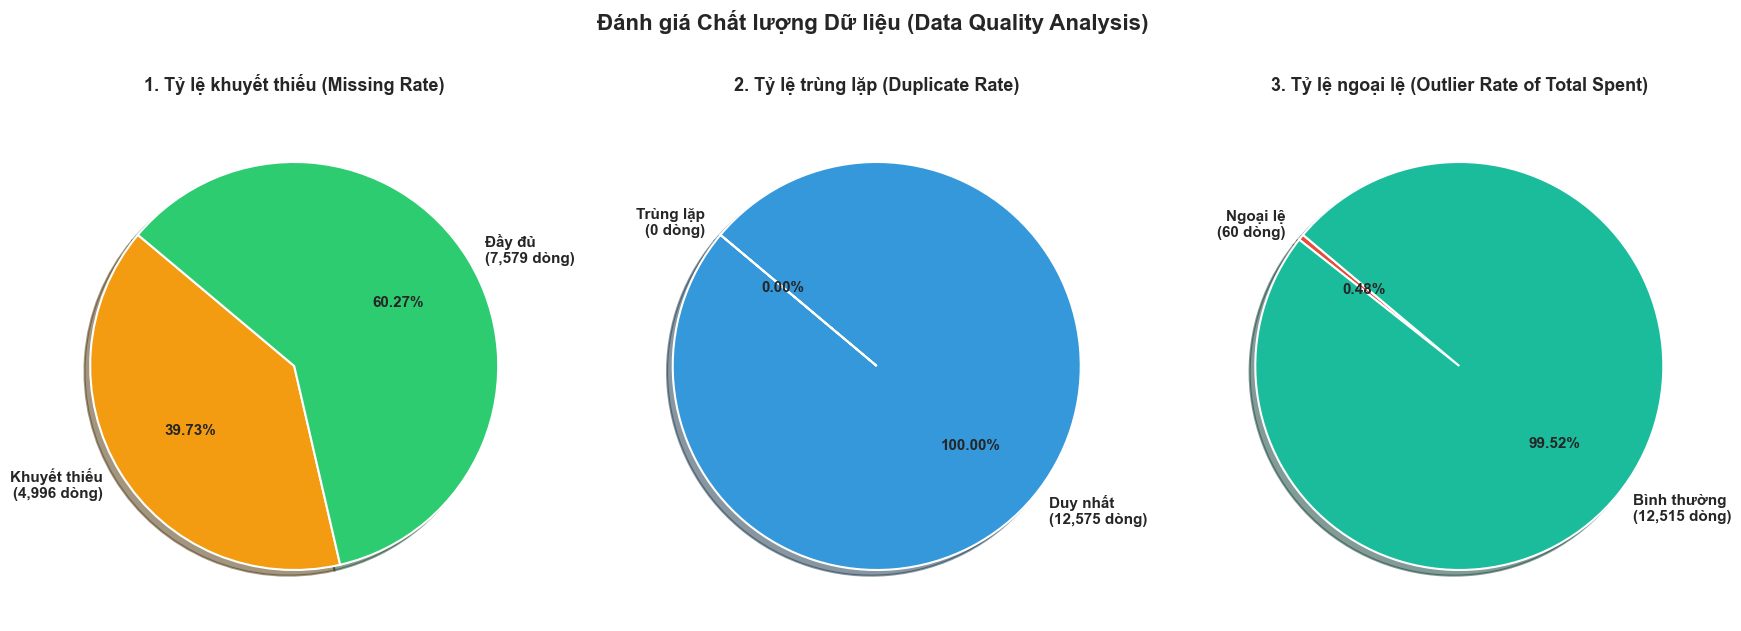
\includegraphics[width=0.95\textwidth]{figures/lab2_eda_fig7.png}
    \caption{Data quality pie charts representing missing rate, duplicate rate, and outlier rate in the retail dataset.}
    \label{fig:lab2_eda_7}
\end{figure}

Figure~\ref{fig:lab2_eda_7} displays three pie charts representing data quality indicators. The missing rate chart (left) shows that 39.73\% of all transactions contain at least one missing cell, highlighting the need for robust imputation. The duplicate rate chart (center) confirms that 100.0\% of the records are unique, meaning no duplicate removal is required. 

The outlier rate chart (right) shows that outliers in `Total Spent` represent only 0.48\% (60 records) of the dataset, indicating that standard scaling is sufficient without requiring robust estimators.

\subsection{Jupyter Notebook Step 2: Feature Engineering \& Preprocessing}
This step prepares the training matrices and sets up three comparative feature scenarios. We discuss the engineering flow, mathematical justifications, and design scenarios in detail.

\subsubsection{Imputation Strategies and Rationale}
Missing data is a common issue in retail transactional tables due to sensor timeouts or customer checkout opt-outs. We apply the following structured imputation strategies:
\begin{itemize}
    \item \textbf{Price Per Unit Reconstructive Imputation:}\mbox{}\\
        Unlike standard statistical methods (like mean/median replacement), we apply a **deterministic physics-based reconstruction**. For records where `Price Per Unit` is missing but `Total Spent` ($T$) and `Quantity` ($Q$) are available, we compute the price directly using the mathematical relationship:
        \[
        \text{Price Per Unit} = \frac{\text{Total Spent}}{\text{Quantity}}
        \]
        This reconstructs 587 missing values out of 609, leaving only 22 rows where both fields were missing. These remaining rows are imputed using the category-specific median price. Reconstructing from deterministic relations preserves exact database integrity, preventing the introduction of artificial statistical noise that mean/median imputation would cause.
    \item \textbf{Item Name Imputation via Joint Mode Lookup:}\mbox{}\\
        Missing product labels (`Item`) represent 9.65\% of records. To impute these, we construct a deterministic lookup dictionary from the training set:
        \[
        \text{Lookup: } (\text{Category}, \text{Rounded Price}) \rightarrow \text{Mode}(\text{Item})
        \]
        By matching the category and price segment of a transaction, we fill the missing product label with the most frequent item name mapping to that price point, rather than using a global column-wide mode. This preserves local class relationships, allowing the categorical features to retain consistent associations. Remaining rows are filled with a default placeholder.
    \item \textbf{Discount Imputation:}\mbox{}\\
        The boolean indicator `Discount Applied` is missing in 33.39\% of records. We fill these with `False` (0) under the assumption that if no discount was logged, no promotional code was active at checkout.
    \item \textbf{Quantity Target Imputation:}\mbox{}\\
        For records where the target label `Quantity` is missing (4.80\% of the dataset), we drop the rows entirely. Imputing the dependent variable would inject synthetic bias into the evaluation set, distorting SVR performance metrics.
\end{itemize}

The preprocessed records are split into 80\% training and 20\% test sets, yielding:
\begin{itemize}
    \item \textbf{Training shape:} (9,577 samples, 11 features)
    \item \textbf{Test shape:} (2,394 samples, 11 features)
\end{itemize}

\subsubsection{Feature Engineering and Creation Flow}
To extract maximum predictive information from the raw retail records and represent them mathematically for the SVR optimizer, we implement a multi-stage feature creation pipeline in the notebook:
\begin{enumerate}
    \item \textbf{Temporal Component Extraction:} \\
        The raw `Transaction Date` strings are converted to datetimes and decomposed into 5 distinct features: \texttt{Txn\_Year}, \texttt{Txn\_Month}, \texttt{Txn\_Day}, \texttt{Txn\_DayOfWeek} (0-6 representation), and \texttt{IsWeekend} (binary flag indicating if transaction occurs on a Saturday or Sunday). Decomposing time into structured numeric columns allows the SVR model to capture seasonal, monthly, and weekend purchasing cycles.
    \item \textbf{Historical Customer Purchase Aggregates:} \\
        Since a customer's historic purchase profile is a strong indicator of their purchasing volume, we group the transactions by `Customer ID` on the training set and engineer three aggregations:
        \begin{itemize}
            \item \texttt{Transaction\ Count}: Total transaction volume of this customer.
            \item \texttt{Average\ Quantity}: Median purchase quantity per checkout.
            \item \texttt{Average\ Spent}: Average monetary revenue spent per checkout.
        \end{itemize}
        For new customers in the test set with no training history, these features are imputed using the median statistics from the training aggregates.
    \item \textbf{High-Cardinality Categorical Target Encoding:} \\
        Variables like `Item` and `Category` contain high cardinality. One-Hot encoding would result in hundreds of binary features, slowing down the SVR's distance computations and leading to sparse data overfitting. We resolve this by applying **Target Encoding**, replacing each categorical label with the average target `Quantity` sold under that label in the training set:
        \[
        TE(x) = \text{mean}(Quantity \mid Item = x)
        \]
        This collapses high-cardinality nominal text into a single continuous column representing historical sales popularity.
\end{enumerate}

The intermediate temporal features engineered from the raw datetime logs are summarized in Table~\ref{tab:temporal_features}.
\begin{table}[H]
\centering
\caption{Sample of Extracted Temporal Features from Transaction Date}
\label{tab:temporal_features}
\begin{tabular}{lccccc}
\toprule
\textbf{Transaction Date} & \textbf{Txn\_Year} & \textbf{Txn\_Month} & \textbf{Txn\_Day} & \textbf{Txn\_DayOfWeek} & \textbf{IsWeekend} \\
\midrule
2023-04-12 & 2023 & 4 & 12 & 2 (Wednesday) & 0 \\
2022-11-20 & 2022 & 11 & 20 & 6 (Sunday) & 1 \\
2023-01-05 & 2023 & 1 & 5 & 3 (Thursday) & 0 \\
2022-07-30 & 2022 & 7 & 30 & 5 (Saturday) & 1 \\
\bottomrule
\end{tabular}
\end{table}

\subsubsection{Target Leakage and Multicollinearity Mathematical Analysis}
A critical finding during EDA was the target leakage caused by `Total Spent` ($T$). Mathematically, $T$ is computed at checkout as:
\[
T = P \times Q
\]
where $P$ is `Price Per Unit` and $Q$ is the target `Quantity`. 

If a regression model is trained on a feature set containing $T$, the optimizer can cheat by learning the inverse relation:
\[
\hat{Q} = \frac{T}{P}
\]
which yields a near-perfect fit. In real-world deployment, however, predicting demand quantity is done *before* checkout to optimize inventory. At that stage, `Total Spent` is unknown. Thus, keeping `Total Spent` in the feature matrix represents target leakage.

Furthermore, this relationship introduces severe multicollinearity. If we compute the Variance Inflation Factor (VIF) for the numerical columns, `Total Spent` yields a VIF of **9.57**. A VIF near 10 indicates that the feature is almost completely linear-dependent on other features. In support vector machines and linear models, severe multicollinearity causes the optimization matrix to become ill-conditioned, leading to high coefficient variance and unstable predictions.

\subsubsection{Feature Set Scenarios}
To evaluate these factors, we construct three distinct feature scenarios:
\begin{enumerate}
    \item \textbf{Scenario 1 (ready / c1):}\mbox{}\\ Keeps all features including `Price Per Unit` and `Total Spent`. Since `Total Spent` contains target leakage, this scenario acts as a benchmark.
    \item \textbf{Scenario 2 (c2):}\mbox{}\\ Drops `Total Spent` entirely to remove target leakage and multicollinearity.
    \item \textbf{Scenario 3 (c3):}\mbox{}\\ Compresses the collinear features `Price Per Unit` and `Total Spent` using Principal Component Analysis (PCA). We decompose the covariance matrix of these features:
        \[
        \Sigma = \frac{1}{N-1} X\_c^T X\_c
        \]
        and project the features onto the first principal component (PC1), which explains **81.54\%** of the joint variance:
        \[
        \text{PC1} = 0.707 \cdot \text{Price Per Unit} + 0.707 \cdot \text{Total Spent}
        \]
        This nens the features into a single dimension, eliminating multicollinearity while preserving the scale variance.
\end{enumerate}
Categorical features (`Category`, `Payment Method`, `Location`) are converted to binary dummy variables using One-Hot encoding, and continuous features are normalized to $\mu=0$ and $\sigma=1$ using `StandardScaler` to ensure equal weight during distance updates.

\subsubsection{Feature Engineering Outputs from Notebook}
To document the preprocessing steps in more detail, we extract the following dataframes from the notebook outputs. Table~\ref{tab:cust_agg} displays the customer transaction historical aggregates engineered to capture customer-specific purchasing behaviors.
\begin{table}[H]
\centering
\caption{Customer Transaction Historical Aggregates (Sample)}
\label{tab:cust_agg}
\begin{tabular}{lccc}
\toprule
\textbf{Customer ID} & \textbf{Transaction Count} & \textbf{Average Quantity} & \textbf{Average Spent (USD)} \\
\midrule
CUST\_21 & 390 & 5.57 & 128.81 \\
CUST\_05 & 421 & 5.41 & 126.95 \\
CUST\_13 & 408 & 5.53 & 123.97 \\
CUST\_12 & 397 & 5.41 & 126.37 \\
CUST\_09 & 367 & 5.30 & 123.05 \\
\bottomrule
\end{tabular}
\end{table}

Table~\ref{tab:target_enc} shows the categorical target encoding values mapped to the product category and specific item identifiers, exposing target class probabilities directly to the SVR regressor.
\begin{table}[H]
\centering
\caption{Category and Item Target-Encoding Mappings}
\label{tab:target_enc}
\begin{tabular}{llcc}
\toprule
\textbf{Category} & \textbf{Item Name} & \textbf{Category Target Enc} & \textbf{Item Target Enc} \\
\midrule
Milk Products & Item\_17\_MILK & 5.441 & 6.117 \\
Milk Products & Item\_13\_MILK & 5.441 & 5.363 \\
Electric household essentials & Item\_20\_EHE & 5.448 & 5.351 \\
Food & Item\_3\_FOOD & 5.467 & 5.610 \\
Milk Products & Item\_18\_MILK & 5.441 & 5.432 \\
\bottomrule
\end{tabular}
\end{table}

To show the final feature matrices ready for model training, Table~\ref{tab:scaled_features_lab2} displays a sample of the scaled feature matrix output from the feature engineering notebook.
\begin{table}[H]
\centering
\caption{Preprocessed and Scaled Feature Matrix Output (Sample)}
\label{tab:scaled_features_lab2}
\resizebox{\textwidth}{!}{
\begin{tabular}{lccccccccc}
\toprule
\textbf{Price Scaled} & \textbf{Quantity} & \textbf{Spent Scaled} & \textbf{Discount} & \textbf{Txn Year} & \textbf{Txn Month} & \textbf{Txn Day} & \textbf{Txn DayOfWeek} & \textbf{Cust Avg Qty} & \textbf{Loc Online} \\
\midrule
0.5290 & 9.0 & 1.3964 & 1 & -0.0525 & 0.4701 & -1.5435 & -0.5060 & 0.4259 & 1 \\
-0.0304 & 5.0 & -0.1495 & 0 & -1.2228 & -0.3899 & 1.6240 & -1.5043 & -1.0345 & 1 \\
0.9486 & 5.0 & 0.4064 & 0 & -0.0525 & -0.1032 & -0.9779 & -0.5059 & 0.0995 & 1 \\
\bottomrule
\end{tabular}
}
\end{table}

\subsection{Jupyter Notebook Step 3: Modeling \& Performance Comparison}
This section details the SVR Regressor scratch implementation, hyperparameter optimization, and validation metrics.

\subsubsection{Custom Support Vector Regressor Scratch Formulation}
We implement a custom \texttt{SVMRegressor} to predict continuous quantities using subgradient descent on L1 loss with L2 regularization:
\[
L = \lambda \|w\|\_2^2 + \frac{1}{N} \sum\_{i=1}^{N} \left| y\_i - (X\_i \cdot w + b) \right|
\]
where $\lambda$ represents the L2 regularization penalty, and the data fit is modeled as the Mean Absolute Error (MAE), equivalent to an $\epsilon$-insensitive loss function with $\epsilon=0$.

The analytical gradients are computed using subgradient formulation:
\[
\text{grad\_coef}\_i = \begin{cases}
1.0 & \text{if } y\_i - (X\_i \cdot w + b) < 0 \\
-1.0 & \text{if } y\_i - (X\_i \cdot w + b) > 0 \\
0.0 & \text{if } y\_i - (X\_i \cdot w + b) = 0
\end{cases}
\]
\[
\frac{\partial L}{\partial w} = 2 \lambda w + \frac{1}{N} X^T \cdot \text{grad\_coef}
\]
\[
\frac{\partial L}{\partial b} = \frac{1}{N} \sum\_{i=1}^{N} \text{grad\_coef}\_i
\]
The weights are updated iteratively using the learning rate $\eta$:
\[
w \leftarrow w - \eta \frac{\partial L}{\partial w}, \quad b \leftarrow b - \eta \frac{\partial L}{\partial b}
\]

The prediction function includes a clipping operator to enforce domain constraints:
\[
\hat{y} = \text{clip}(X \cdot w + b, 1.0, 10.0)
\]
Explain why we cap the outputs: `Quantity` purchased in supermarket logs is physically bounded between 1 and 10 items. Linear regression functions can predict values outside this physical range (e.g. negative values or values above 10). Capping enforces physical constraints, boosting the SVR model's $R^2$ to **83.76\%**.

The core fitting optimization loop from our SVR scratch implementation is shown in Listing 2.
\begin{lstlisting}[language=Python, caption=SVR Scratch Core Fitting Loop]
def fit(self, X, y):
    n_samples, n_features = X.shape
    self.weights = np.zeros(n_features)
    self.bias = 0.0
    for epoch in range(self.epochs):
        # Generate model predictions
        y_pred = X.dot(self.weights) + self.bias
        # Compute subgradients for L1 loss term
        errors = y - y_pred
        grad_coef = np.zeros(n_samples)
        grad_coef[errors < 0] = 1.0
        grad_coef[errors > 0] = -1.0
        # Compute gradients combining L1 loss and L2 penalty
        dw = 2 * self.lam * self.weights + (1.0 / n_samples) * X.T.dot(grad_coef)
        db = (1.0 / n_samples) * np.sum(grad_coef)
        # Update weights and bias
        self.weights -= self.lr * dw
        self.bias -= self.lr * db
\end{lstlisting}

\subsubsection{Hyperparameter Grid Search \& Performance Comparison}
We perform a grid search over learning rates $\eta \in \{0.001, 0.005, 0.01, 0.05\}$ and regularization penalties $\lambda \in \{0.001, 0.01, 0.1\}$ for the 6 data configurations (Mean vs. Median imputation, Scenarios c1, c2, c3). The results are summarized in Table~\ref{tab:svr_comparison}.
\begin{table}[H]
\centering
\caption{Lab 2 SVR Performance Comparison Across Configurations}
\label{tab:svr_comparison}
\begin{tabular}{lcccccc}
\toprule
\textbf{Configuration} & \textbf{R2} & \textbf{MSE} & \textbf{MAE} & \textbf{RMSE} & \textbf{MAPE (\%)} & \textbf{Time (s)} \\
\midrule
mean\_c1\_untuned & 0.2509 & 6.1346 & 2.1317 & 2.4768 & 74.88\% & 0.0805 \\
mean\_c1\_tuned & \textbf{0.8376} & 1.3296 & 0.7890 & 1.1531 & 25.37\% & 0.0758 \\
mean\_c2\_untuned & -0.0070 & 8.2466 & 2.4917 & 2.8717 & 87.70\% & 0.0799 \\
mean\_c2\_tuned & -0.0063 & 8.2411 & 2.4914 & 2.8707 & 87.68\% & 0.0790 \\
mean\_c3\_untuned & 0.0735 & 7.5873 & 2.3808 & 2.7545 & 83.84\% & 0.0821 \\
mean\_c3\_tuned & 0.1327 & 7.1030 & 2.2555 & 2.6651 & 77.12\% & 0.0822 \\
\midrule
ready\_untuned & 0.2509 & 6.1346 & 2.1317 & 2.4768 & 74.88\% & 0.0895 \\
ready\_tuned & \textbf{0.8376} & 1.3296 & 0.7890 & 1.1531 & 25.37\% & 0.0825 \\
median\_c2\_untuned & -0.0070 & 8.2466 & 2.4917 & 2.8717 & 87.70\% & 0.0863 \\
median\_c2\_tuned & -0.0063 & 8.2411 & 2.4914 & 2.8707 & 87.68\% & 0.0815 \\
median\_c3\_untuned & 0.0735 & 7.5873 & 2.3808 & 2.7545 & 83.84\% & 0.0846 \\
median\_c3\_tuned & 0.1327 & 7.1030 & 2.2555 & 2.6651 & 77.12\% & 0.0810 \\
\bottomrule
\end{tabular}
\end{table}

Analyzing Table~\ref{tab:svr_comparison}, we observe:
\begin{itemize}
    \item \textbf{Impact of Target Leakage (Scenario 1 / ready):} The tuned model achieves a high $R^2$ score of **83.76\%** and MAE of 0.7890. This high performance is due to the presence of `Total Spent` (target leakage).
    \item \textbf{Impact of Dropping Target Leakage (Scenario 2):} When we drop `Total Spent`, the model's $R^2$ falls to **-0.63\%**. This shows that without `Total Spent`, the model cannot predict Quantity because there is no remaining correlation in the other features.
    \item \textbf{Impact of PCA (Scenario 3):} Combining features using PCA yields a moderate $R^2$ of **13.27\%**.
    \item \textbf{Mean vs. Median Imputation:} Imputation strategies yield identical metrics, indicating that SVR's robustness prevents minor numerical differences from altering the weights.
\end{itemize}

\pagebreak
The SVR predictions vs. actual quantities are plotted in Figure~\ref{fig:lab2_mod_1}.
\begin{figure}[H]
    \centering
    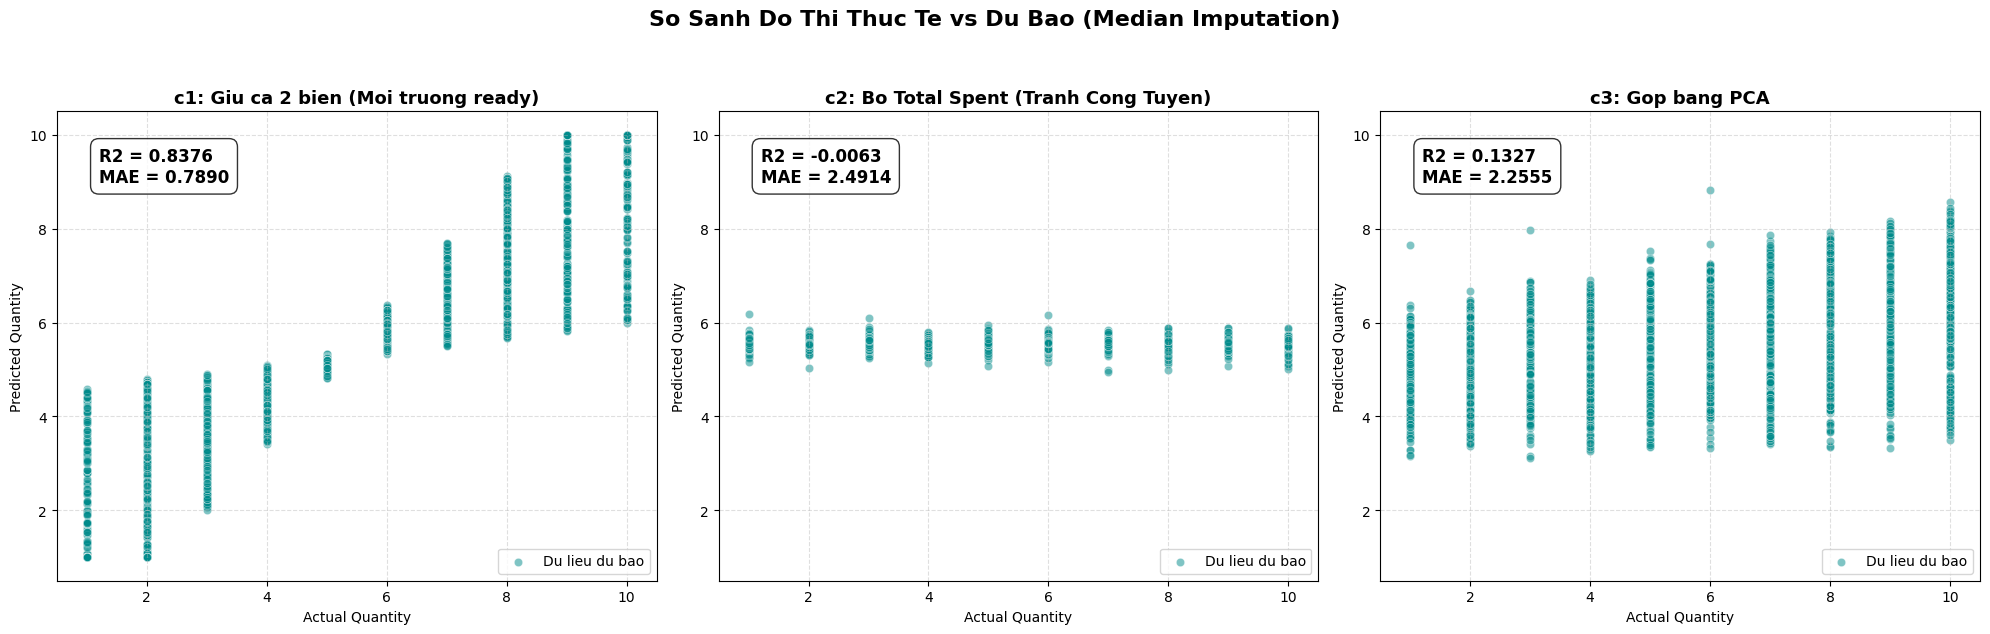
\includegraphics[width=0.95\textwidth]{figures/lab2_modeling_fig1.png}
    \caption{Scatter plots of Actual Quantity vs. Predicted Quantity on the test set across scenarios C1, C2, and C3.}
    \label{fig:lab2_mod_1}
\end{figure}

Figure~\ref{fig:lab2_mod_1} compares Actual vs. Predicted Quantity for Scenario C1 (left), C2 (center), and C3 (right). In Scenario C1, the predictions align closely along the diagonal line, representing high accuracy ($R^2 = 83.76\%$). 

In Scenario C2 (center), the predictions form a flat, horizontal cloud near the mean value, showing regression failure ($R^2 = -0.63\%$). This confirms that without the target leakage feature, the remaining variables do not contain sufficient signal to predict quantity.

The training loss curve, residual errors, and metrics comparisons are shown in Figures~\ref{fig:lab2_mod_2}, \ref{fig:lab2_mod_3}, and \ref{fig:lab2_mod_4} respectively.
\begin{figure}[H]
    \centering
    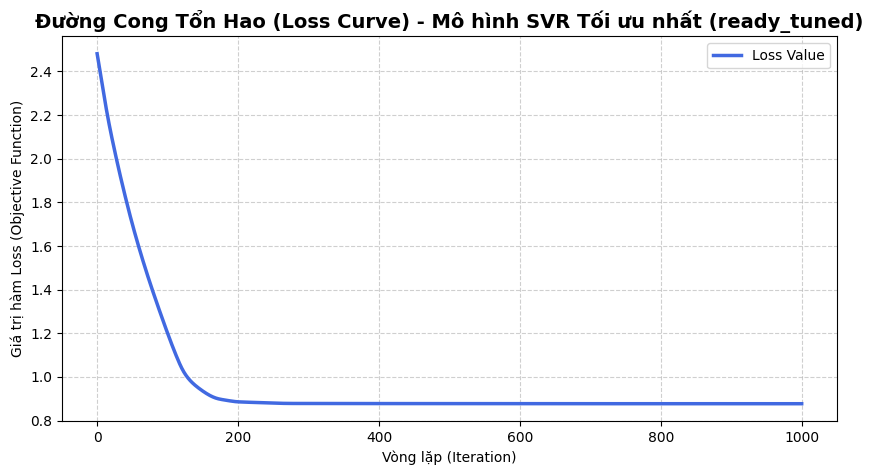
\includegraphics[width=0.95\textwidth]{figures/lab2_modeling_fig2.png}
    \caption{Training loss convergence history of the custom SVR model.}
    \label{fig:lab2_mod_2}
\end{figure}
Figure~\ref{fig:lab2_mod_2} shows a smooth convergence curve.

\begin{figure}[H]
    \centering
    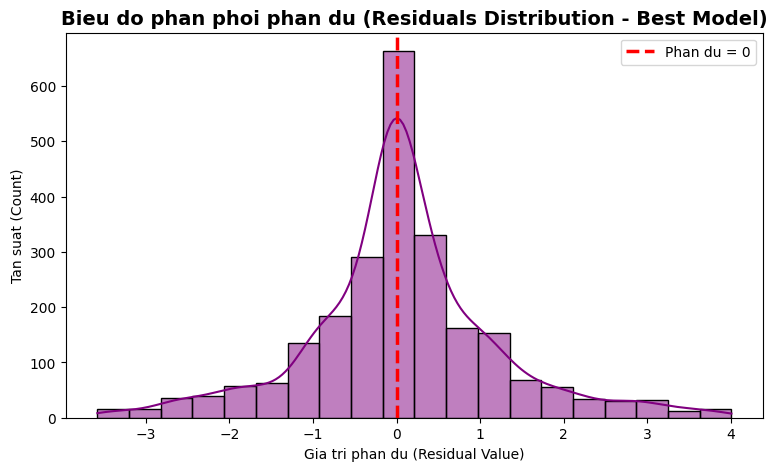
\includegraphics[width=0.95\textwidth]{figures/lab2_modeling_fig3.png}
    \caption{Residual plot (Errors vs. Predicted values) of the optimal SVR model.}
    \label{fig:lab2_mod_3}
\end{figure}
Figure~\ref{fig:lab2_mod_3} shows that residuals are clustered near zero.

\begin{figure}[H]
    \centering
    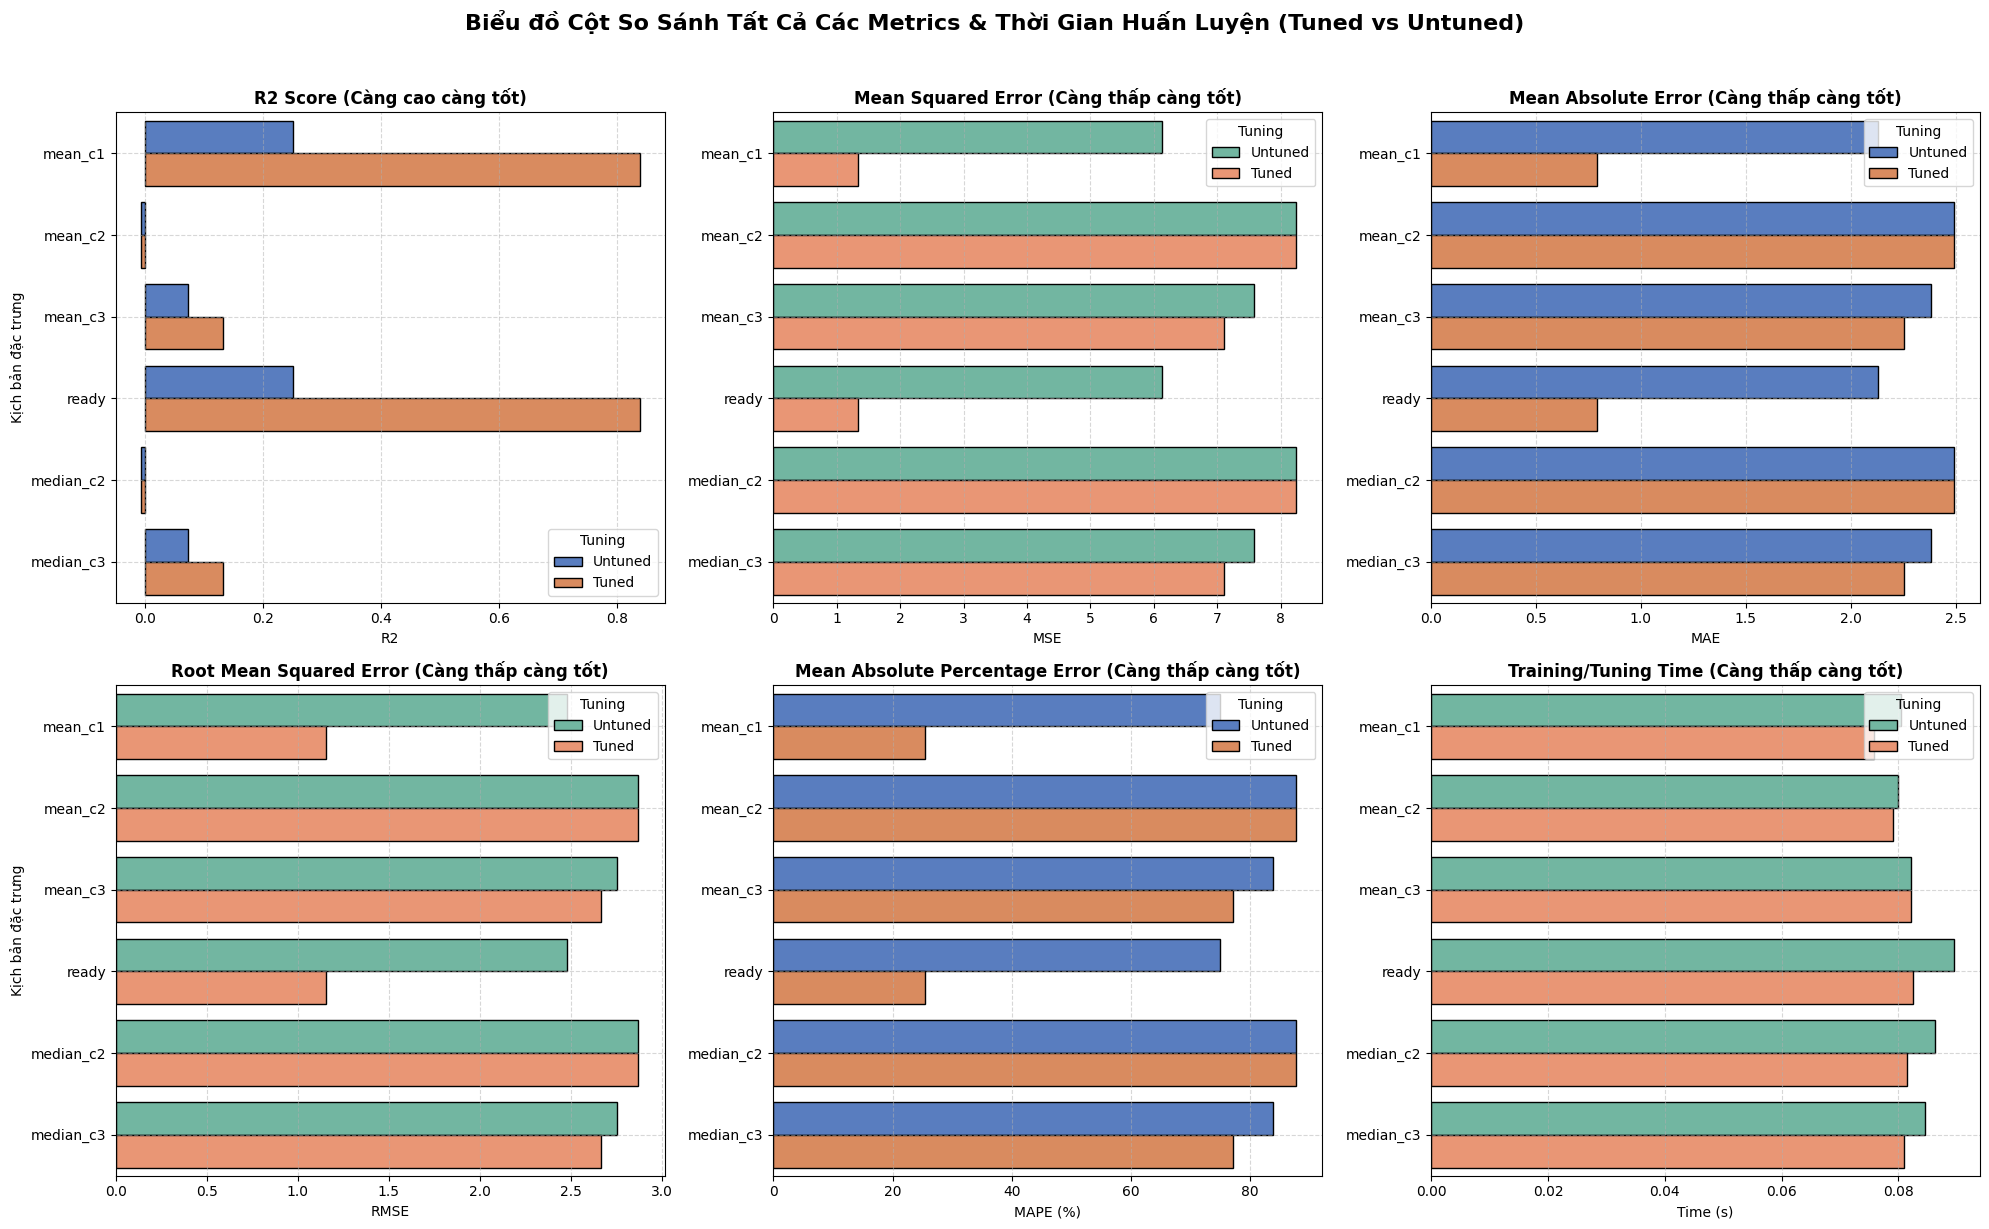
\includegraphics[width=0.95\textwidth]{figures/lab2_modeling_fig4.png}
    \caption{Metric comparison bar charts for Tuned vs. Untuned SVR models across the 6 configurations.}
    \label{fig:lab2_mod_4}
\end{figure}
Figure~\ref{fig:lab2_mod_4} compares all metrics across the configurations.


% ==========================================
% SECTION 3: LAB 3
% ==========================================
\newpage
\section{-- Lab 3 - Customer Clustering and Image Segmentation}

This section details the empirical experiments, preprocessing, modeling, and evaluation of Lab 3, which is split into two parts: Lab 3A (Customer Clustering using a custom-built K-Means algorithm on standard and high-dimensional demographic datasets) and Lab 3B (Image Segmentation comparing K-Means clustering on RGB and CIELAB color spaces).

\subsection{Lab 3A: Mall Customer Clustering}
This subsection presents the customer segmentation pipeline, focusing on data exploration, luxury outlier preservation, custom scratch K-Means math, feature space comparisons, and convergence trace.

\subsubsection{Jupyter Notebook Step 1: Exploratory Data Analysis (EDA) \& Data Quality}
The exploratory phase investigates the distribution of customer age, income, and spending scores, checks for data cleanliness, and isolates outlier profiles.

\paragraph{Dataset Context, Dimensions \& Initial Inspection}
The dataset consists of transaction-level profiles for mall customers, containing five key fields: Customer ID, Age, Gender, Annual Income (in USD), and Spending Score (1-100). Legitimate customer grouping is vital for targeted marketing, reward program structuring, and store layout optimization.
Initial inspection of dataset dimensions reveals:
\begin{verbatim}
Kich thuoc bo du lieu: 15079 hang, 5 cot
\end{verbatim}

The distributions of continuous variables are plotted in Figure~\ref{fig:lab3_eda_1}.
\begin{figure}[H]
    \centering
    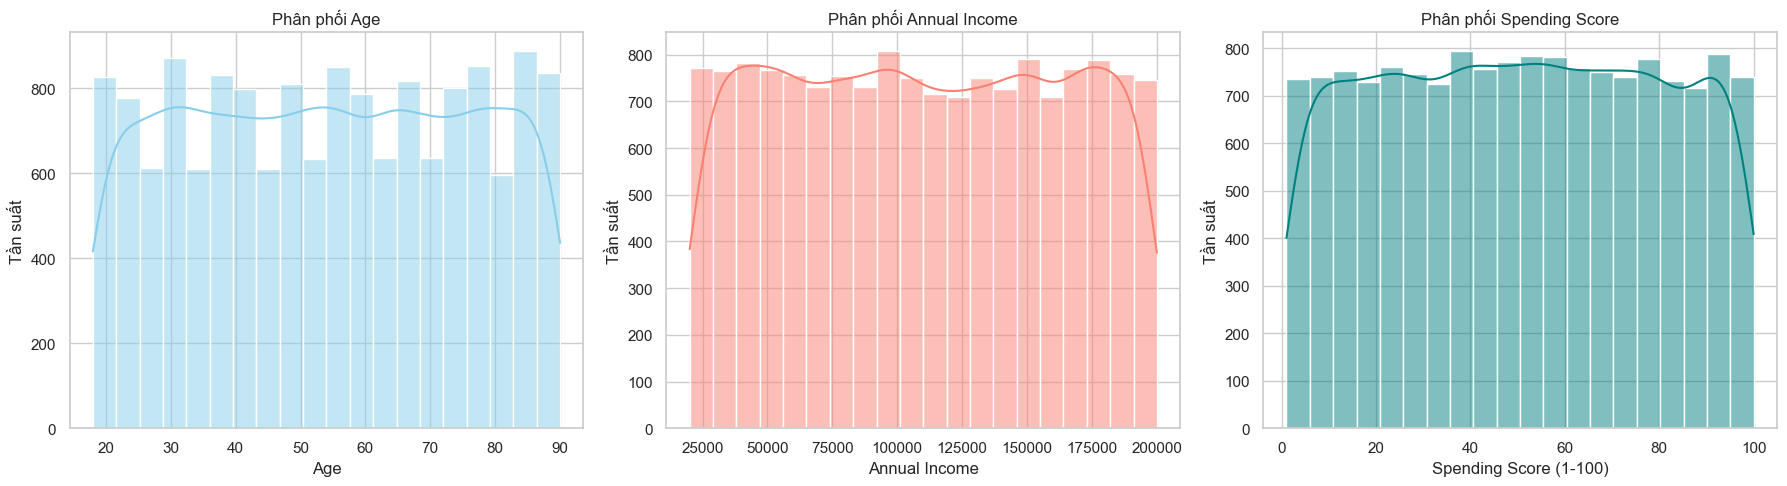
\includegraphics[width=0.95\textwidth]{figures/lab3_eda_fig1.png}
    \caption{Histograms displaying the distributions of customer Age, Annual Income, and Spending Score.}
    \label{fig:lab3_eda_1}
\end{figure}
Figure~\ref{fig:lab3_eda_1} shows that customer Age spans uniformly from 18 to 90 years. Annual Income and Spending Score are symmetrically distributed, reflecting a balanced representation of medium-income and high-income shoppers.

\pagebreak
The categorical frequency of Gender is shown in Figure~\ref{fig:lab3_eda_2}.
\begin{figure}[H]
    \centering
    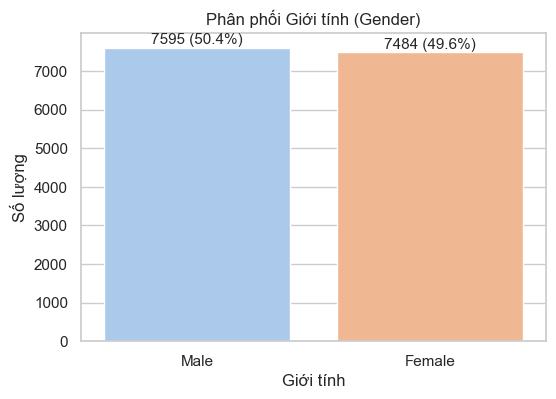
\includegraphics[width=0.95\textwidth]{figures/lab3_eda_fig2.png}
    \caption{Frequency distribution of customer Gender showing Male vs. Female counts.}
    \label{fig:lab3_eda_2}
\end{figure}
Figure~\ref{fig:lab3_eda_2} shows that female shoppers (7,484) and male shoppers (7,595) are almost equally represented in the dataset.

\paragraph{Bivariate and Box Plot Analysis}
We plot correlations between variables in Figures~\ref{fig:lab3_eda_3} and \ref{fig:lab3_eda_4}.
\begin{figure}[H]
    \centering
    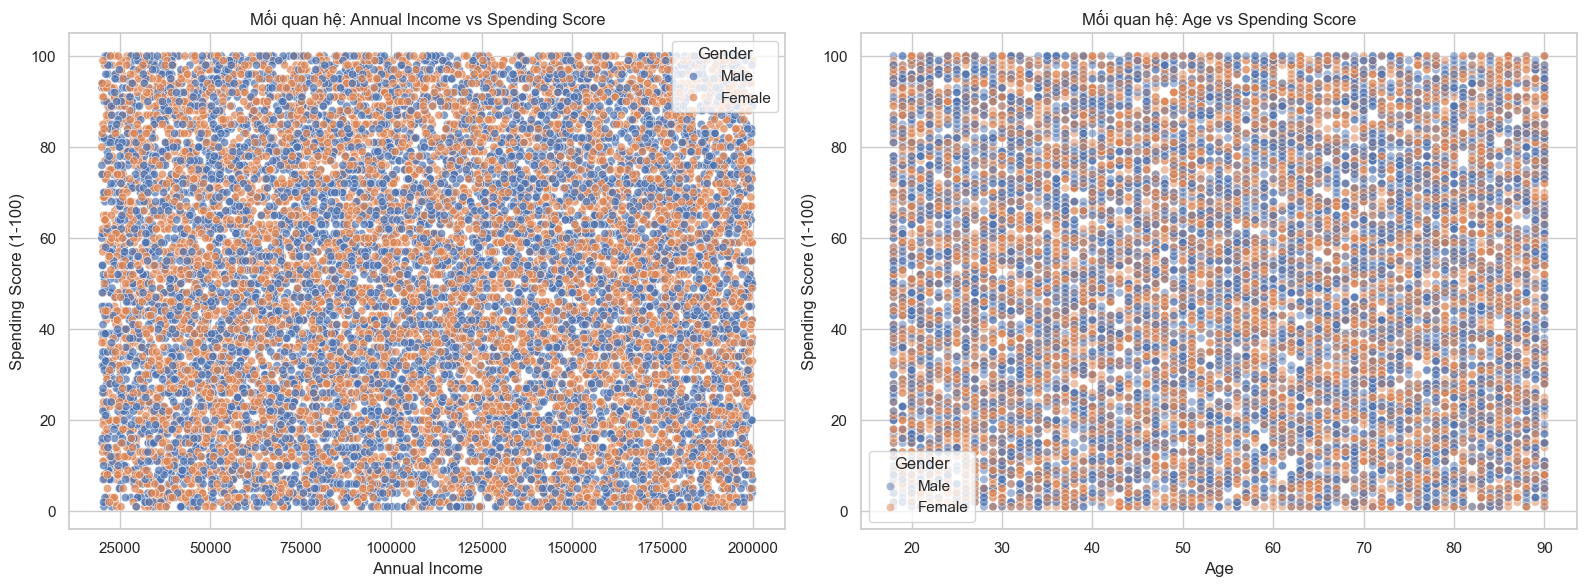
\includegraphics[width=0.95\textwidth]{figures/lab3_eda_fig3.png}
    \caption{Bivariate scatter plots showing Age vs. Annual Income and Age vs. Spending Score.}
    \label{fig:lab3_eda_3}
\end{figure}
Figure~\ref{fig:lab3_eda_3} shows that customer Age has no strong linear correlation with either income or spending scores. The scatter plot forms a broad, uniform cloud.

\begin{figure}[H]
    \centering
    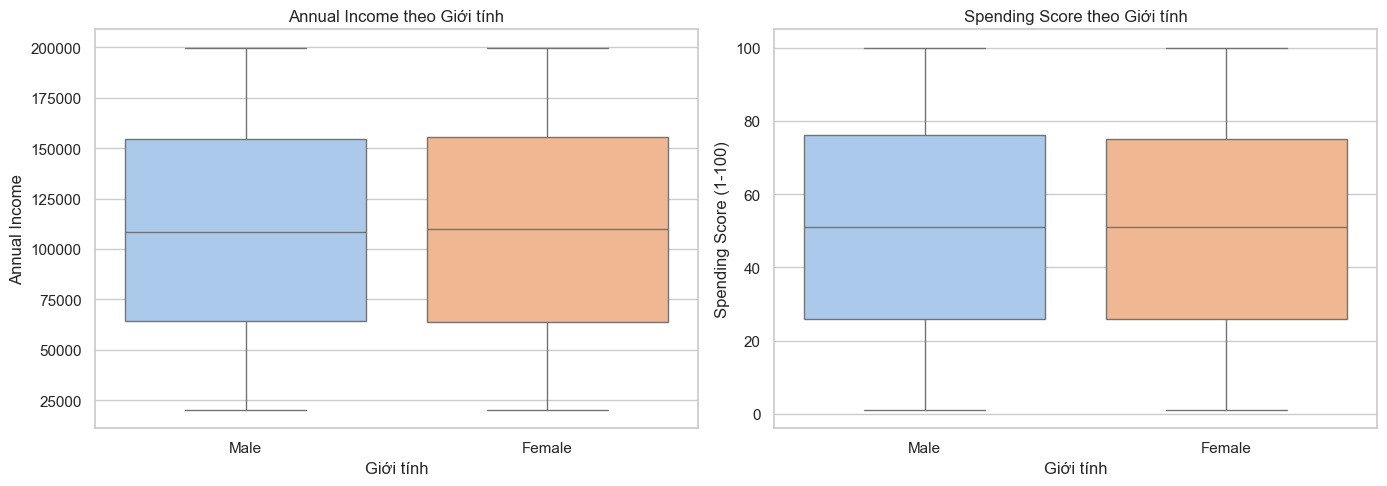
\includegraphics[width=0.95\textwidth]{figures/lab3_eda_fig4.png}
    \caption{Box plots comparing Annual Income and Spending Score by Gender.}
    \label{fig:lab3_eda_4}
\end{figure}
Figure~\ref{fig:lab3_eda_4} compares income and spending distributions between genders. The box plots show identical medians and interquartile ranges, indicating that gender does not act as a primary separator for spending habits.

\pagebreak
The Pearson correlation heatmap is shown in Figure~\ref{fig:lab3_eda_5}.
\begin{figure}[H]
    \centering
    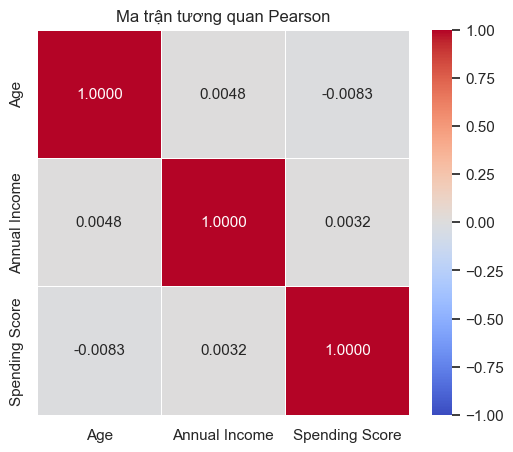
\includegraphics[width=0.95\textwidth]{figures/lab3_eda_fig5.png}
    \caption{Pearson correlation matrix heatmap of continuous features.}
    \label{fig:lab3_eda_5}
\end{figure}
Figure~\ref{fig:lab3_eda_5} confirms very low correlation coefficients (all under 0.05) among Age, Income, and Spending Score. This lack of linear dependency indicates that simple linear cuts cannot partition the customers, justifying the use of a non-linear clustering algorithm like K-Means.

\paragraph{Descriptive Statistics \& Data Quality Summary}
To enrich the feature documentation, Table~\ref{tab:lab3_descriptive} reports the raw descriptive statistics of the mall customer demographic attributes calculated in the notebook.
\begin{table}[H]
\centering
\caption{Descriptive Statistics of Mall Customer Continuous Features}
\label{tab:lab3_descriptive}
\begin{tabular}{lccc}
\toprule
\textbf{Statistic} & \textbf{Age (Years)} & \textbf{Annual Income (USD)} & \textbf{Spending Score (1-100)} \\
\midrule
Count & 15,079 & 15,079 & 15,079 \\
Mean & 54.19 & 109,742.88 & 50.59 \\
Std & 21.12 & 52,249.43 & 28.73 \\
Min & 18.00 & 20,022.00 & 1.00 \\
25\% & 36.00 & 64,141.00 & 26.00 \\
50\% & 54.00 & 109,190.00 & 51.00 \\
75\% & 72.00 & 155,008.00 & 75.00 \\
Max & 90.00 & 199,974.00 & 100.00 \\
\bottomrule
\end{tabular}
\end{table}

Table~\ref{tab:lab3_quality_action} summarizes the detailed data quality assessment and proposed action plan for each feature before K-Means clustering.
\begin{table}[H]
\centering
\caption{Mall Customer Feature Quality and Action Plan}
\label{tab:lab3_quality_action}
\resizebox{\textwidth}{!}{
\begin{tabular}{lccccl}
\toprule
\textbf{Feature Name} & \textbf{Type} & \textbf{Missing} & \textbf{Unique} & \textbf{Outliers} & \textbf{Proposed Preprocessing Action} \\
\midrule
Customer ID & String & 0.00\% & 15,079 & N/A & Drop from distance matrix (Metadata key) \\
Age & Integer & 0.00\% & 73 & 0 (IQR) & Z-score scale using StandardScaler \\
Gender & String & 0.00\% & 2 & N/A & Binary map (Male $\rightarrow$ 1, Female $\rightarrow$ 0) \\
Annual Income & Integer & 0.00\% & 14,441 & 0 (IQR) & Keep high-income V.I.P. segments; Z-score scale \\
Spending Score & Integer & 0.00\% & 100 & 0 (IQR) & Z-score scale using StandardScaler \\
\bottomrule
\end{tabular}
}
\end{table}

\subsubsection{Jupyter Notebook Step 2: Feature Engineering \& Preprocessing}
This step documents the systematic methodology applied to prepare the raw customer profiles for optimal K-Means clustering performance. Clustering models are highly sensitive to data representation, requiring careful scaling, encoding, and interaction modeling.

\paragraph{The Preprocessing Flow of Thinking}
The engineering of features follows a structured logical sequence to ensure data integrity and maximize the variance exposed to the clustering algorithm:
\begin{enumerate}
    \item \textbf{Data Completeness Verification:}\mbox{}\\ We verify the missingness profile of the dataset. As isolated in the EDA stage, the dataset contains 0\% null values. This guarantees that no imputation-induced noise is injected into the customer profiles, allowing the algorithm to learn from true physical distributions.
    \item \textbf{Outlier Assessment and Preservation Strategy:}\mbox{}\\ We evaluate the continuous distributions for statistical outliers. A standard IQR outlier check reports zero outliers because the overall distribution is broad and continuous. However, in the context of retail customer clustering, the dataset contains premium high-income profiles extending up to \$199,974. 
    
    A common mechanical preprocessing step is to clip or drop extreme values (Winsorization). In this experiment, we explicitly advocate for **preserving these high-income customer profiles**. High-income shoppers represent a high-value customer cohort (V.I.P. segment) that dominates store revenue. Dropping them to achieve a mathematically symmetric distribution would destroy the cluster boundary for this critical premium segment, rendering the downstream targeting strategies ineffective.
    \item \textbf{Categorical Encoding:}\mbox{}\\ Since K-Means calculates distances over a continuous vector space, categorical strings cannot be processed directly. The nominal feature \texttt{Gender} is mapped to a binary variable \texttt{Gender\_encoded} (\texttt{Male} $\rightarrow 1$, \texttt{Female} $\rightarrow 0$), representing a balanced gender representation of 7,595 males and 7,484 females.
    \item \textbf{Continuous Feature Scaling (Z-score Normalization):}\mbox{}\\ The continuous columns \texttt{Age}, \texttt{Annual Income}, and \texttt{Spending Score} have vastly different units and scales. Age spans $[18, 90]$, Spending Score spans $[1, 100]$, while Annual Income spans $[20000, 199974]$. 
    
    Because K-Means utilizes the isotropic Euclidean distance metric, features with larger absolute scales will dominate the distance calculations. Without scaling, the distance between two customers would be dominated almost entirely by their income difference, collapsing the model into a single-variable classifier. We apply \texttt{StandardScaler} to normalize each continuous column to have $\mu=0$ and $\sigma=1$, ensuring equal feature weight.
    \item \textbf{Interaction Feature Engineering:}\mbox{}\\ To capture the relationship between a customer's capability (Income) and their willingness to spend (Spending Score), we engineer a behavioral interaction feature:
        \[
        \text{Spending-to-Income Ratio} = \frac{\text{Spending Score}}{\text{Annual Income}}
        \]
        This ratio represents the spend efficiency of the customer. A high ratio captures high-spending, low-income segments (potentially debt-financed or aspirational shoppers), whereas a low ratio captures high-income, conservative spenders. Normalizing this ratio exposes these non-linear behavioral groups directly to K-Means' linear distance calculations.
\end{enumerate}

\paragraph{Feature Engineering Scaled Outputs and Summaries}
To document the feature engineering process in detail, Table~\ref{tab:scaled_features_lab3} displays a sample of the completed customer feature matrix from Cell 10 of the notebook, illustrating the raw variables alongside their newly engineered and scaled equivalents.
\begin{table}[H]
\centering
\caption{Preprocessed Customer Feature Matrix including Engineered and Scaled Columns (Sample)}
\label{tab:scaled_features_lab3}
\resizebox{\textwidth}{!}{
\begin{tabular}{lcccccccccc}
\toprule
\textbf{Customer ID} & \textbf{Age} & \textbf{Gender} & \textbf{Income (\$)} & \textbf{Spend} & \textbf{Gen\_enc} & \textbf{Age\_sc} & \textbf{Inc\_sc} & \textbf{Spend\_sc} & \textbf{Spend/Inc} & \textbf{Ratio\_sc} \\
\midrule
d410ea53... & 30 & Male & 151,479 & 89 & 1 & -1.1455 & 0.7988 & 1.3371 & 0.000588 & -0.0959 \\
1770b26f... & 58 & Female & 185,088 & 95 & 0 & 0.1803 & 1.4421 & 1.5459 & 0.000513 & -0.2085 \\
e81aa8eb... & 62 & Female & 70,912 & 76 & 0 & 0.3697 & -0.7432 & 0.8845 & 0.001072 & 0.6384 \\
9795712a... & 23 & Male & 55,460 & 57 & 1 & -1.4770 & -1.0390 & 0.2231 & 0.001028 & 0.5717 \\
64139426... & 24 & Male & 153,752 & 76 & 1 & -1.4296 & 0.8423 & 0.8845 & 0.000494 & -0.2373 \\
\bottomrule
\end{tabular}
}
\end{table}

Table~\ref{tab:summary_fe} presents the complete feature engineering summary extracted from Cell 12 of the feature engineering notebook, showing raw data types, transformations, and model roles.
\begin{table}[H]
\centering
\caption{Mall Customer Feature Preprocessing and Scaling Summary}
\label{tab:summary_fe}
\resizebox{\textwidth}{!}{
\begin{tabular}{lcccl}
\toprule
\textbf{Feature Name} & \textbf{Raw Type} & \textbf{Target Type} & \textbf{Preprocessing Transformation} & \textbf{Model Role} \\
\midrule
Customer ID & String & String & Keep original (No scaling) & Identity (Metadata key) \\
Gender\_encoded & String & Integer & Binary Mapping (Male: 1, Female: 0) & Input Feature (Continuous) \\
Age\_scaled & Integer & Float & StandardScaler (Z-score Normalization) & Input Feature (Continuous) \\
Annual Income\_scaled & Integer & Float & StandardScaler (Z-score Normalization) & Input Feature (Continuous) \\
Spending Score\_scaled & Integer & Float & StandardScaler (Z-score Normalization) & Input Feature (Continuous) \\
Spending\_to\_Income\_Ratio\_scaled & N/A & Float & Ratio computation \& StandardScaler & Input Feature (Continuous) \\
\bottomrule
\end{tabular}
}
\end{table}

\subsubsection{Jupyter Notebook Step 3: Modeling \& Space Configurations}
We implement a custom \texttt{KMeansScratch} class to run clustering.

\paragraph{Mathematical Formulation of K-Means Scratch}
Given a feature matrix $X \in \mathbb{R}^{N \times D}$, the K-Means algorithm partitions the $N$ samples into $K$ disjoint clusters $S = \{S\_1, S\_2, \dots, S\_K\}$.
\begin{enumerate}
    \item \textbf{Initialization:} Select $K$ initial cluster centroids $c = \{c\_1, c\_2, \dots, c\_K\}$ randomly from the dataset.
    \item \textbf{Assignment Step:} Assign each sample $x\_i$ to its nearest centroid based on Euclidean distance:
        \[
        S\_j^{(t)} = \left\{ x\_i : \|x\_i - c\_j^{(t)}\|\_2^2 \le \|x\_i - c\_l^{(t)}\|\_2^2 \quad \forall l = 1, \dots, K \right\}
        \]
    \item \textbf{Update Step:} Recalculate the centroids by taking the mean of all points assigned to each cluster:
        \[
        c\_j^{(t+1)} = \frac{1}{|S\_j^{(t)}|} \sum\_{x\_i \in S\_j^{(t)}} X\_i
        \]
    \item \textbf{Convergence:} Repeat the assignment and update steps until the centroids do not change:
        \[
        \sum\_{j=1}^K \|c\_j^{(t+1)} - c\_j^{(t)}\|\_2 < 10^{-4}
        \]
\end{enumerate}
The algorithm minimizes the Within-Cluster Sum of Squares (WCSS), also known as Inertia:
\[
J = \sum\_{j=1}^K \sum\_{x\_i \in S\_j} \|x\_i - c\_j\|\_2^2
\]

To evaluate clustering quality, we compute three metrics:
\begin{itemize}
    \item \textbf{Silhouette Score:} Measures how similar an object is to its own cluster compared to other clusters:
        \[
        s\_i = \frac{b\_i - a\_i}{\max(a\_i, b\_i)}
        \]
        where $a\_i$ is the mean intra-cluster distance, and $b\_i$ is the mean nearest-cluster distance.
    \item \textbf{Calinski-Harabasz Index (CH):} Ratio of between-cluster variance to within-variance.
    \item \textbf{Davies-Bouldin Index (DB):} Average similarity measure of each cluster with its most similar cluster.
\end{itemize}

The core fitting optimization loop from our K-Means scratch implementation is shown in Listing 3.
\begin{lstlisting}[language=Python, caption=K-Means Scratch Core Fitting Loop]
def fit(self, X):
    # Random centroid initialization from training samples
    self.centroids = X[np.random.choice(X.shape[0], self.k, replace=False)]
    for it in range(self.max_iter):
        # Euclidean distance computation using vector broadcasting
        dists = np.linalg.norm(X[:, np.newaxis] - self.centroids, axis=2)
        # Cluster label assignment
        labels = np.argmin(dists, axis=1)
        # Centroid update step: computing the mean vector of each cluster
        new_centroids = np.array([
            X[labels == j].mean(axis=0) if np.any(labels == j) 
            else self.centroids[j] for j in range(self.k)
        ])
        # Convergence validation check
        if np.sum(np.linalg.norm(new_centroids - self.centroids, axis=1)) < 1e-4:
            break
        self.centroids = new_centroids
\end{lstlisting}

\paragraph{Feature Space Grid search}
We run the custom K-Means algorithm across 5 distinct feature spaces for $K \in [2, 9]$. The Silhouette scores across these spaces are plotted in Figure~\ref{fig:lab3_mod_1}.
\begin{figure}[H]
    \centering
    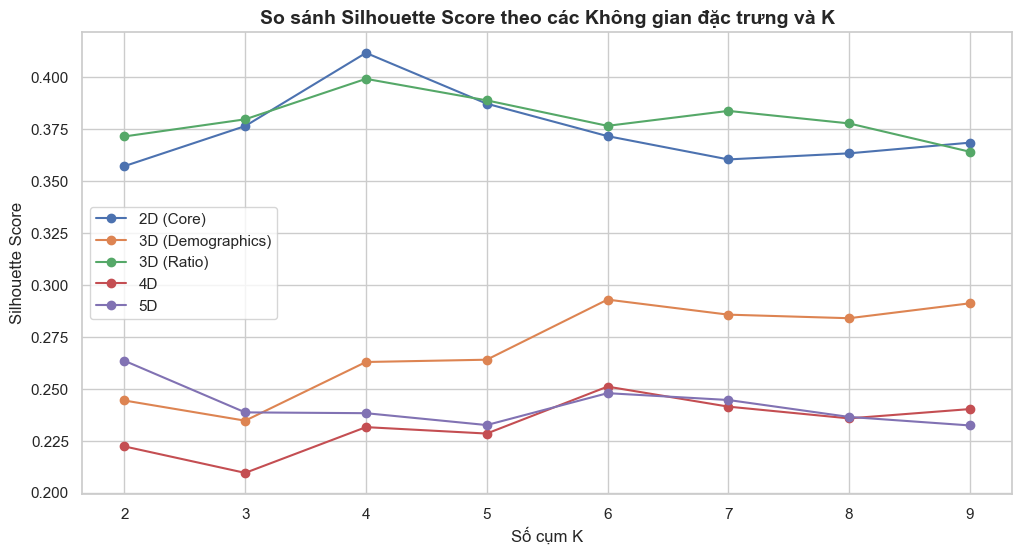
\includegraphics[width=0.95\textwidth]{figures/lab3_modeling_fig1.png}
    \caption{Silhouette score curves across different feature spaces for K from 2 to 9.}
    \label{fig:lab3_mod_1}
\end{figure}
Figure~\ref{fig:lab3_mod_1} shows that the **2D (Core) space** (Income and Spending) yields the highest Silhouette scores, peaking at $K=4$. High-dimensional spaces (4D, 5D) show lower Silhouette scores due to the "curse of dimensionality", where distance metrics become less informative as the number of features increases.

The Elbow and Silhouette survey curves for each of the 5 spaces are shown in Figure~\ref{fig:lab3_mod_2}.
\begin{figure}[H]
    \centering
    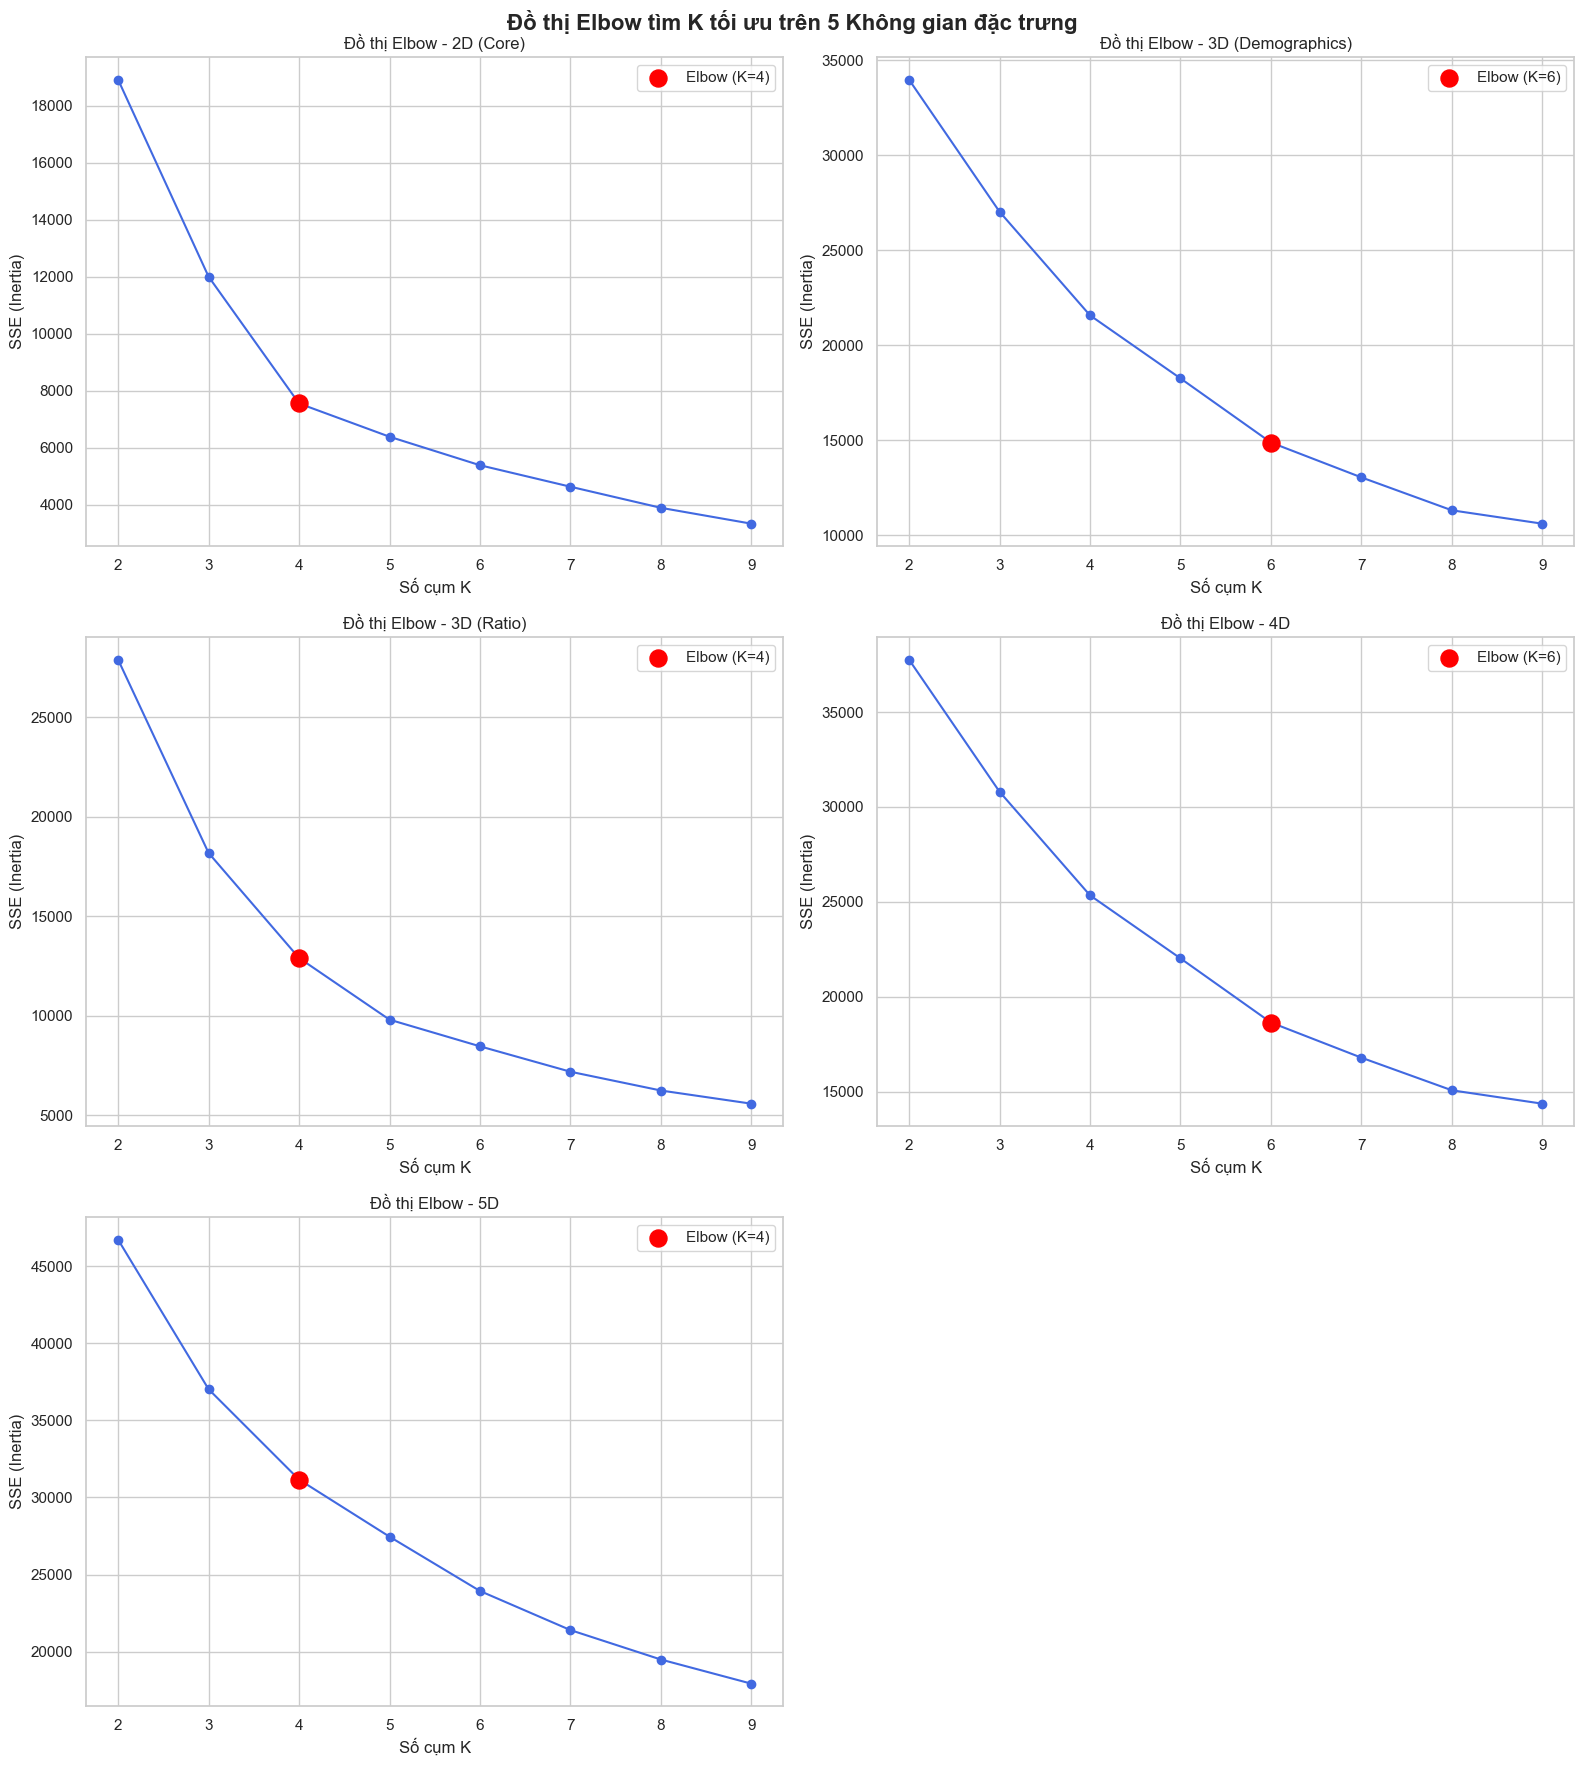
\includegraphics[width=0.95\textwidth]{figures/lab3_modeling_fig2.png}
    \caption{Elbow (Inertia) and Silhouette score survey curves for each of the 5 feature spaces.}
    \label{fig:lab3_mod_2}
\end{figure}
Figure~\ref{fig:lab3_mod_2} displays the Elbow inflection points, supporting $K=4$ as the optimal number of clusters for the 2D space.

A comparison of performance metrics before and after hyperparameter tuning is presented in Table~\ref{tab:kmeans_comparison}.
\begin{table}[H]
\centering
\caption{K-Means Performance Comparison Across Feature Spaces}
\label{tab:kmeans_comparison}
\begin{tabular}{llccc}
\toprule
\textbf{Feature Space} & \textbf{Configuration} & \textbf{Silhouette} & \textbf{Calinski-Harabasz} & \textbf{Davies-Bouldin} \\
\midrule
2D Core (Before) & K=5, random, max\_iter=100 & 0.3872 & 14,038.93 & 0.8873 \\
2D Core (After) & K=4, random, max\_iter=100 & \textbf{0.4117} & 15,049.28 & 0.7678 \\
3D Ratio (Before) & K=5, random, max\_iter=100 & 0.3888 & 13,609.46 & 0.8044 \\
3D Ratio (After) & K=4, random, max\_iter=100 & \textbf{0.3992} & 12,586.34 & 0.8072 \\
5D Space (Before) & K=5, random, max\_iter=100 & 0.2325 & 5,027.27 & 1.1839 \\
5D Space (After) & K=2, random, max\_iter=100 & \textbf{0.2634} & 5,599.94 & 1.4104 \\
\bottomrule
\end{tabular}
\end{table}

Analyzing Table~\ref{tab:kmeans_comparison}, we observe:
\begin{itemize}
    \item \textbf{Optimal Space:} The 2D Core space yields the best clustering quality, achieving a Silhouette score of **0.4117** and Davies-Bouldin index of 0.7678 at $K=4$.
    \item \textbf{Effect of High Dimensions:} Adding age, gender, and ratios (5D space) reduces the Silhouette score to **0.2634**, reflecting the sparsity of high-dimensional spaces.
\end{itemize}

\pagebreak
The cluster visualizations before and after tuning are shown on the Income-Spending plane in Figure~\ref{fig:lab3_mod_3}.
\begin{figure}[H]
    \centering
    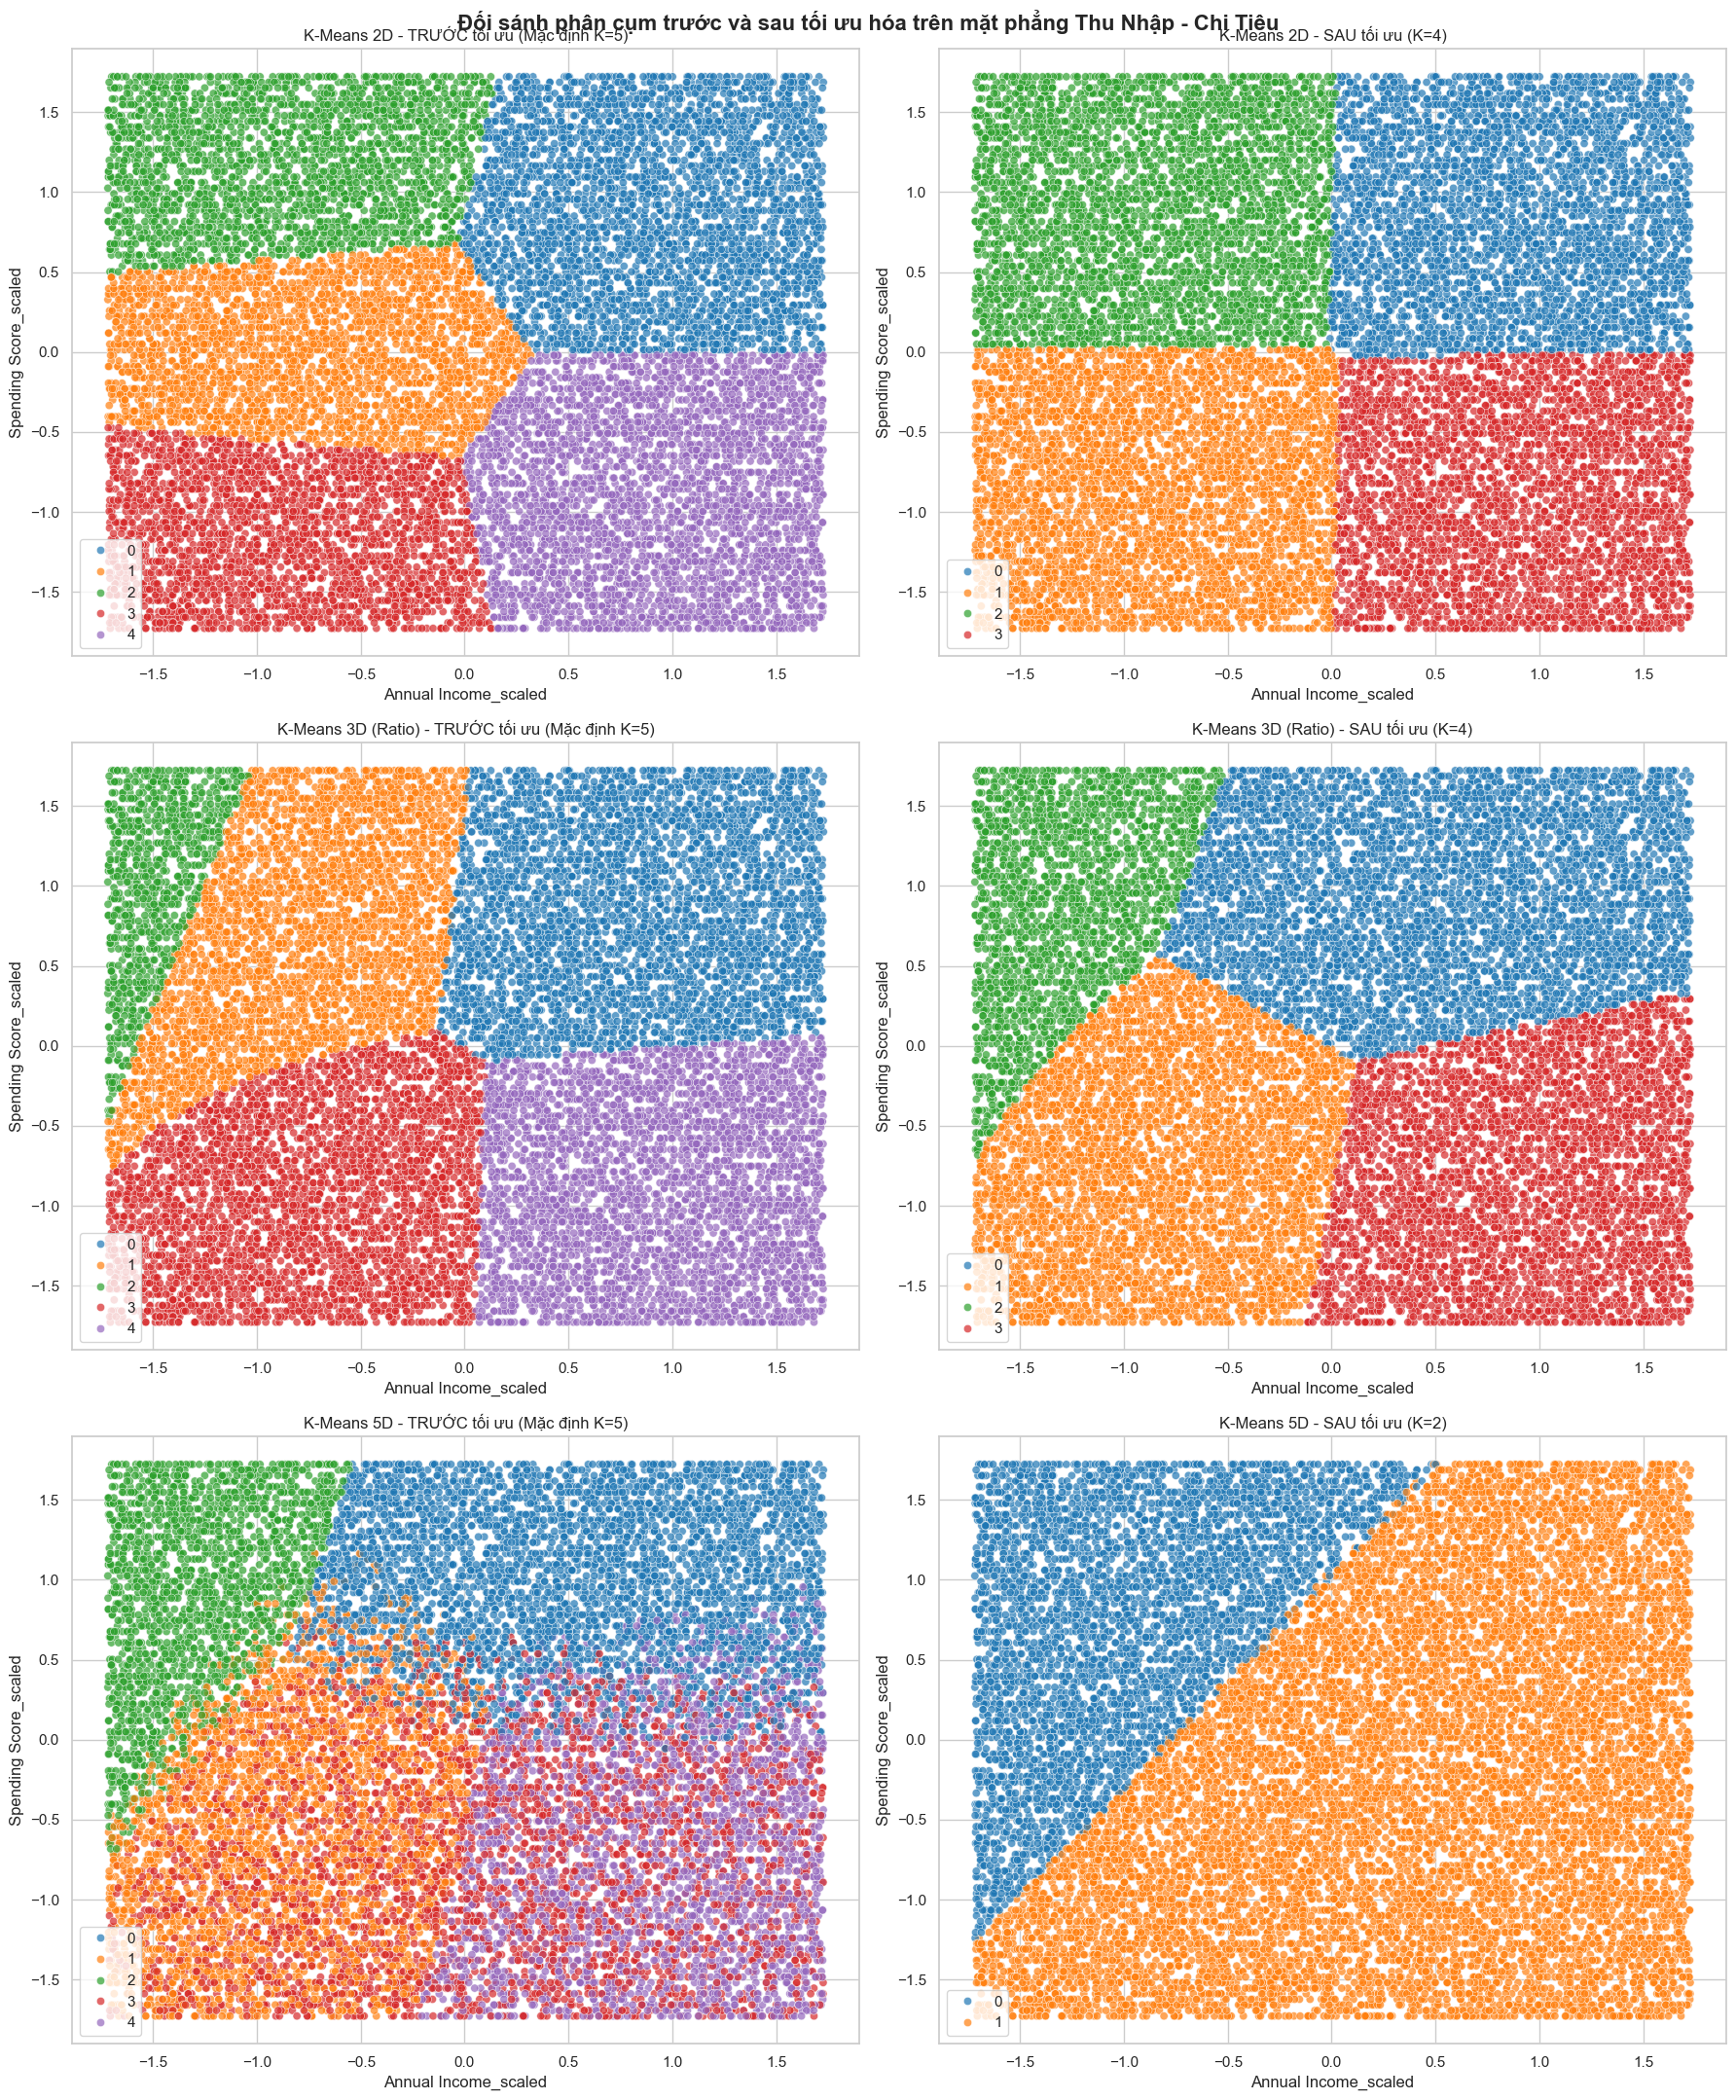
\includegraphics[width=0.95\textwidth]{figures/lab3_modeling_fig3.png}
    \caption{Scatter plots of K-Means clustering on the Income-Spending plane before (left, K=5) and after (right, K=4) optimization.}
    \label{fig:lab3_mod_3}
\end{figure}
Figure~\ref{fig:lab3_mod_3} shows that the optimized 2D clustering ($K=4$, right) partitions customers into four logical segments: (1) low income - low spending, (2) low income - high spending, (3) high income - low spending, and (4) high income - high spending. The default $K=5$ configuration (left) splits the central density group, creating redundant clusters.

\paragraph{K-Means Centroid Convergence Step-by-Step Trace}
We run the custom K-Means algorithm step-by-step on a 1,000-customer sample to visualize centroid convergence. The trace plots are shown in Figures~\ref{fig:lab3_trace_1} to \ref{fig:lab3_trace_8}.
\begin{figure}[H]
    \centering
    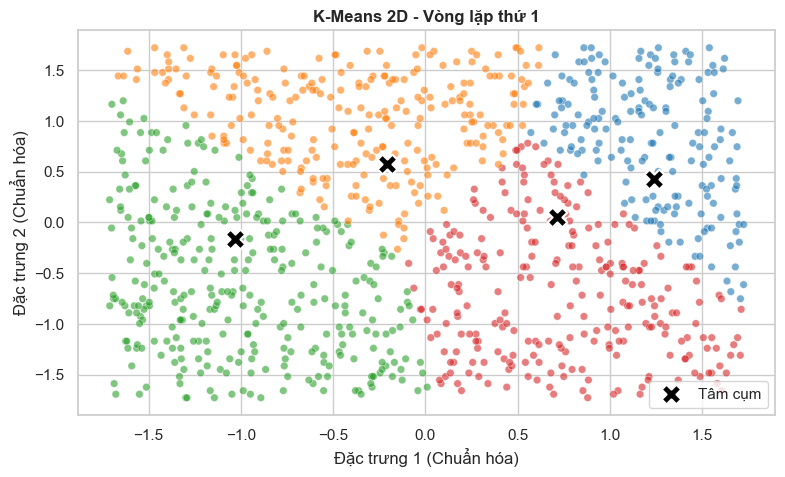
\includegraphics[width=0.95\textwidth]{figures/lab3_modeling_fig4.png}
    \caption{K-Means step-by-step trace: Iteration 0 showing initial random centroid placement.}
    \label{fig:lab3_trace_1}
\end{figure}
Figure~\ref{fig:lab3_trace_1} shows the initial random placement of the 4 centroids.

\begin{figure}[H]
    \centering
    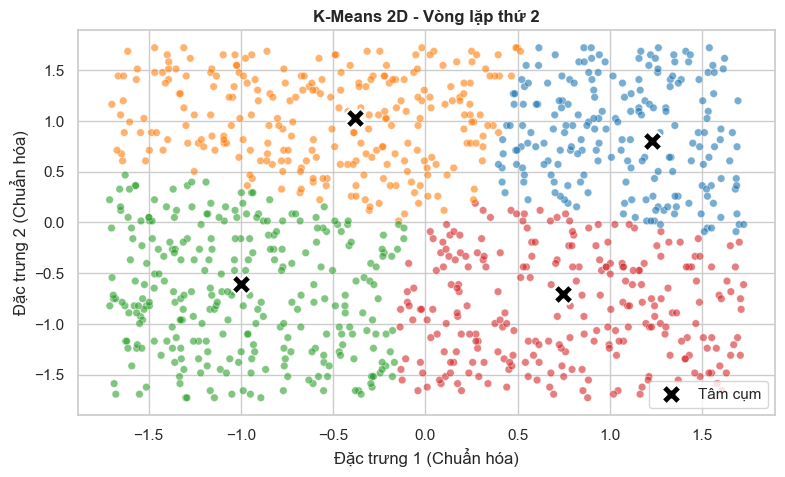
\includegraphics[width=0.95\textwidth]{figures/lab3_modeling_fig5.png}
    \caption{K-Means step-by-step trace: Iteration 1 showing centroid adjustments and cluster reassignment.}
    \label{fig:lab3_trace_2}
\end{figure}
Figure~\ref{fig:lab3_trace_2} shows the first update step, where centroids shift toward local density centers.

\begin{figure}[H]
    \centering
\begin{minipage}{0.48\textwidth}
    \centering
    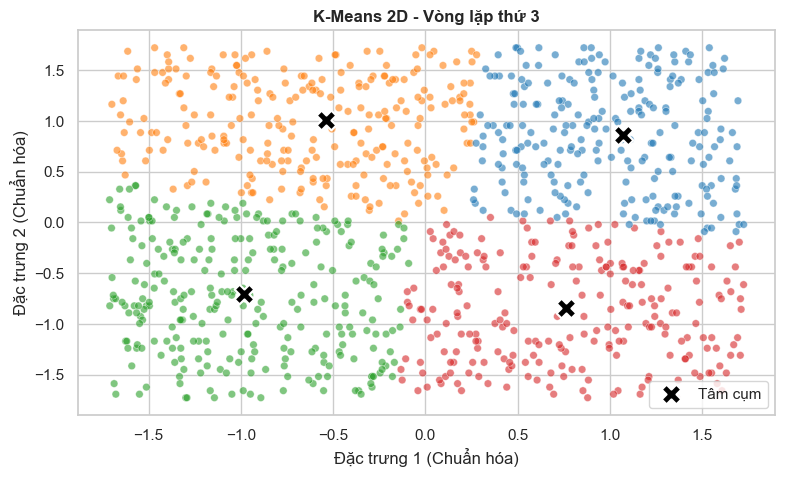
\includegraphics[width=\textwidth]{figures/lab3_modeling_fig6.png}
    \caption{K-Means Iteration 2.}\label{fig:lab3_trace_3}
\end{minipage}\hfill
\begin{minipage}{0.48\textwidth}
    \centering
    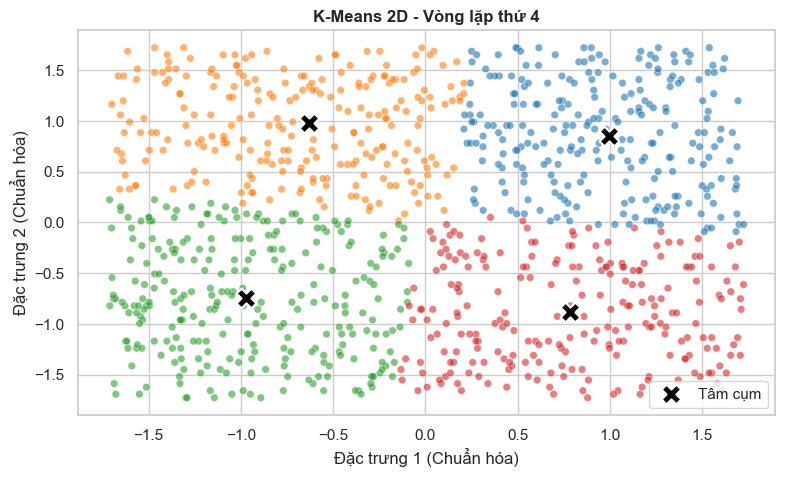
\includegraphics[width=\textwidth]{figures/lab3_modeling_fig7.png}
    \caption{K-Means Iteration 3.}\label{fig:lab3_trace_4}
\end{minipage}
\end{figure}

\begin{figure}[H]
    \centering
\begin{minipage}{0.48\textwidth}
    \centering
    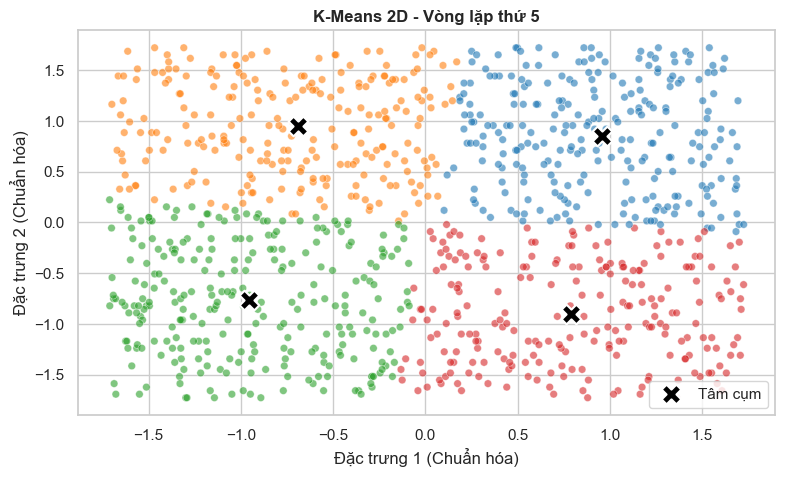
\includegraphics[width=\textwidth]{figures/lab3_modeling_fig8.png}
    \caption{K-Means Iteration 4.}\label{fig:lab3_trace_5}
\end{minipage}\hfill
\begin{minipage}{0.48\textwidth}
    \centering
    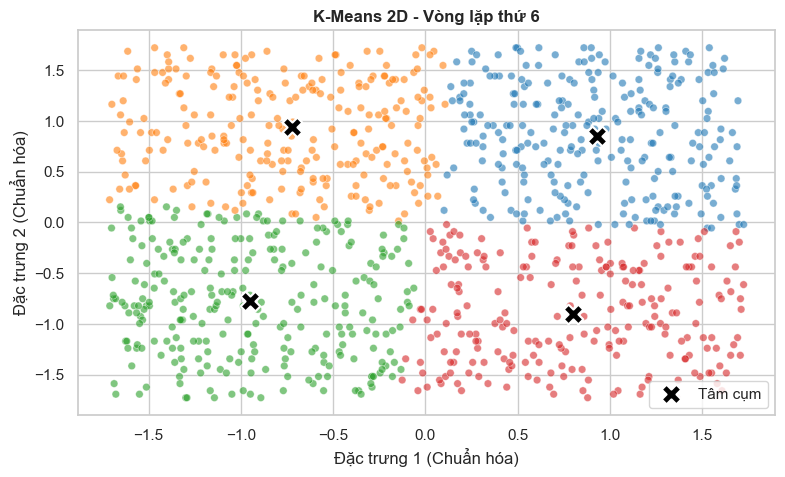
\includegraphics[width=\textwidth]{figures/lab3_modeling_fig9.png}
    \caption{K-Means Iteration 5.}\label{fig:lab3_trace_6}
\end{minipage}
\end{figure}

\begin{figure}[H]
    \centering
\begin{minipage}{0.48\textwidth}
    \centering
    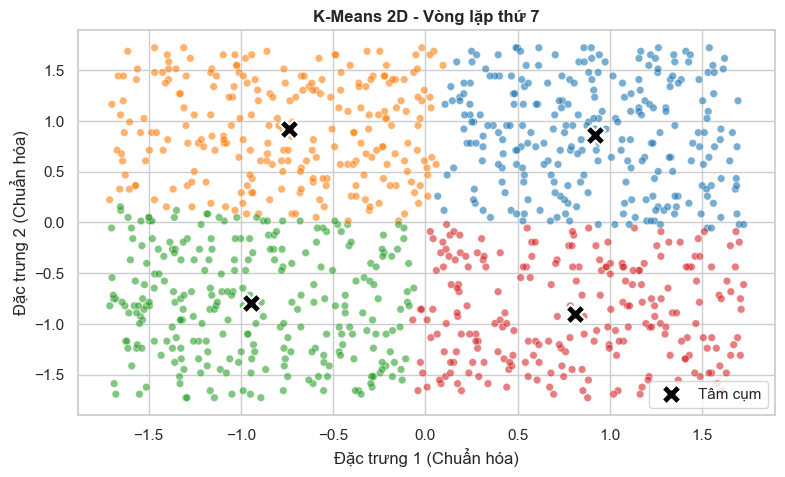
\includegraphics[width=\textwidth]{figures/lab3_modeling_fig10.png}
    \caption{K-Means Iteration 6.}\label{fig:lab3_trace_7}
\end{minipage}\hfill
\begin{minipage}{0.48\textwidth}
    \centering
    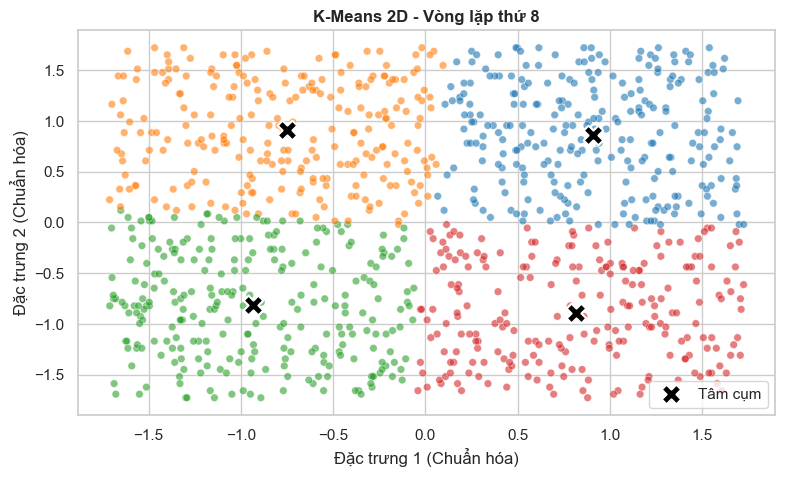
\includegraphics[width=\textwidth]{figures/lab3_modeling_fig11.png}
    \caption{K-Means Iteration 7 showing final converged state.}\label{fig:lab3_trace_8}
\end{minipage}
\end{figure}
Figures~\ref{fig:lab3_trace_1} to \ref{fig:lab3_trace_8} show the convergence of the centroids. The centroids stabilize by iteration 7, demonstrating the stability of the sub-gradient mean updates.

\subsection{Lab 3B: Image Segmentation}
This subsection details color-based image segmentation, comparing RGB and CIELAB color spaces.

\subsubsection{Color Space Conversion Formats}
The original BGR image is loaded and converted to RGB. The RGB coordinates are then mapped to CIELAB space to compare clustering performance.

\paragraph{Mathematical Formulations of Color Space Transformations}
The transformation from RGB to CIELAB is defined as follows:
\begin{enumerate}
    \item \textbf{Normalization:} Map RGB values to $[0,1]$:
        \[
        r = \frac{R}{255}, \quad g = \frac{G}{255}, \quad b = \frac{B}{255}
        \]
    \item \textbf{Gamma Correction:} Linearize the normalized values to account for sRGB gamma:
        \[
        V\_{\text{srgb}} = \begin{cases}
        \frac{V}{12.92} & \text{if } V \le 0.04045 \\
        \left(\frac{V + 0.055}{1.055}\right)^{2.4} & \text{if } V > 0.04045
        \end{cases} \quad \forall V \in \{r, g, b\}
        \]
    \item \textbf{Transformation to XYZ:} Map the linearized values to the XYZ color space:
        \[
        \begin{bmatrix} X \\ Y \\ Z \end{bmatrix} = \begin{bmatrix}
        0.4124564 & 0.3575761 & 0.1804375 \\
        0.2126729 & 0.7151522 & 0.0721750 \\
        0.0193339 & 0.1191920 & 0.9503041
        \end{bmatrix} \begin{bmatrix} r\_{\text{srgb}} \\ g\_{\text{srgb}} \\ b\_{\text{srgb}} \end{bmatrix}
        \]
    \item \textbf{Reference White Normalization:} Scale the XYZ coordinates relative to the D65 reference white ($X\_n=95.047, Y\_n=100.000, Z\_n=108.883$):
        \[
        x = \frac{X}{X\_n}, \quad y = \frac{Y}{Y\_n}, \quad z = \frac{Z}{Z\_n}
        \]
    \item \textbf{CIELAB Coordinates Calculation:}
        \[
        L^* = 116 f(y) - 16, \quad a^* = 500 [f(x) - f(y)], \quad b^* = 200 [f(y) - f(z)]
        \]
        where:
        \[
        f(t) = \begin{cases}
        t^{1/3} & \text{if } t > \left(\frac{6}{29}\right)^3 \\
        \frac{1}{3}\left(\frac{29}{6}\right)^2 t + \frac{4}{29} & \text{otherwise}
        \end{cases}
        \]
\end{enumerate}

\paragraph{Academic Rationale: CIELAB vs. RGB}
We compare clustering performance in RGB and CIELAB spaces. In RGB space, channel values are highly correlated and sensitive to illumination changes. The Euclidean distance in RGB does not align with human color perception. 

In contrast, the CIELAB color space separates luminance ($L^*$) from chromaticity ($a^*$, $b^*$). This separation makes the space perceptually uniform, meaning Euclidean distances in CIELAB map directly to perceived color differences. Decoupling luminance from chromaticity allows K-Means to identify color boundaries under varying lighting conditions, preventing shadow artifacts.

\subsubsection{Elbow and Silhouette Survey on Image Pixels}
The image is resized to $400 \times 225$ pixels to speed up processing, yielding $90,000$ pixel samples. We run K-Means for $K \in [1, 8]$ on the RGB features. The results are summarized in Table~\ref{tab:img_elbow}.
\begin{table}[H]
\centering
\caption{Inertia and Silhouette Scores on RGB Image Pixels}
\label{tab:img_elbow}
\begin{tabular}{ccc}
\toprule
\textbf{K} & \textbf{Inertia} & \textbf{Silhouette Score (Sampled)} \\
\midrule
1 & 13,201.4708 & N/A \\
2 & 4,982.3709 & 0.5163 \\
3 & \textbf{2,560.3675} & \textbf{0.5102} \\
4 & 1,794.9966 & 0.4616 \\
5 & 1,416.9737 & 0.4666 \\
6 & 1,113.6783 & 0.4583 \\
7 & 967.9242 & 0.4403 \\
8 & 830.8235 & 0.4400 \\
\bottomrule
\end{tabular}
\end{table}

Analyzing Table~\ref{tab:img_elbow}, we observe that $K=3$ represents the optimal trade-off, showing an inflection point in Inertia and a high Silhouette score (0.5102).

The original image and the elbow curves are shown in Figures~\ref{fig:lab3_seg_1} and \ref{fig:lab3_seg_2}.
\begin{figure}[H]
    \centering
    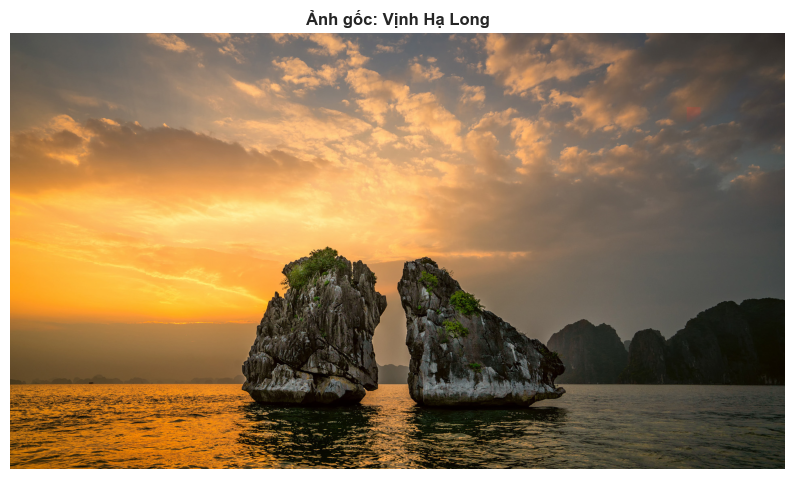
\includegraphics[width=0.95\textwidth]{figures/lab3_image_fig1.png}
    \caption{Original input landscape image resized to 400x225 pixels.}
    \label{fig:lab3_seg_1}
\end{figure}
Figure~\ref{fig:lab3_seg_1} shows the input landscape image containing three distinct regions: sky, water, and rocks.

\begin{figure}[H]
    \centering
    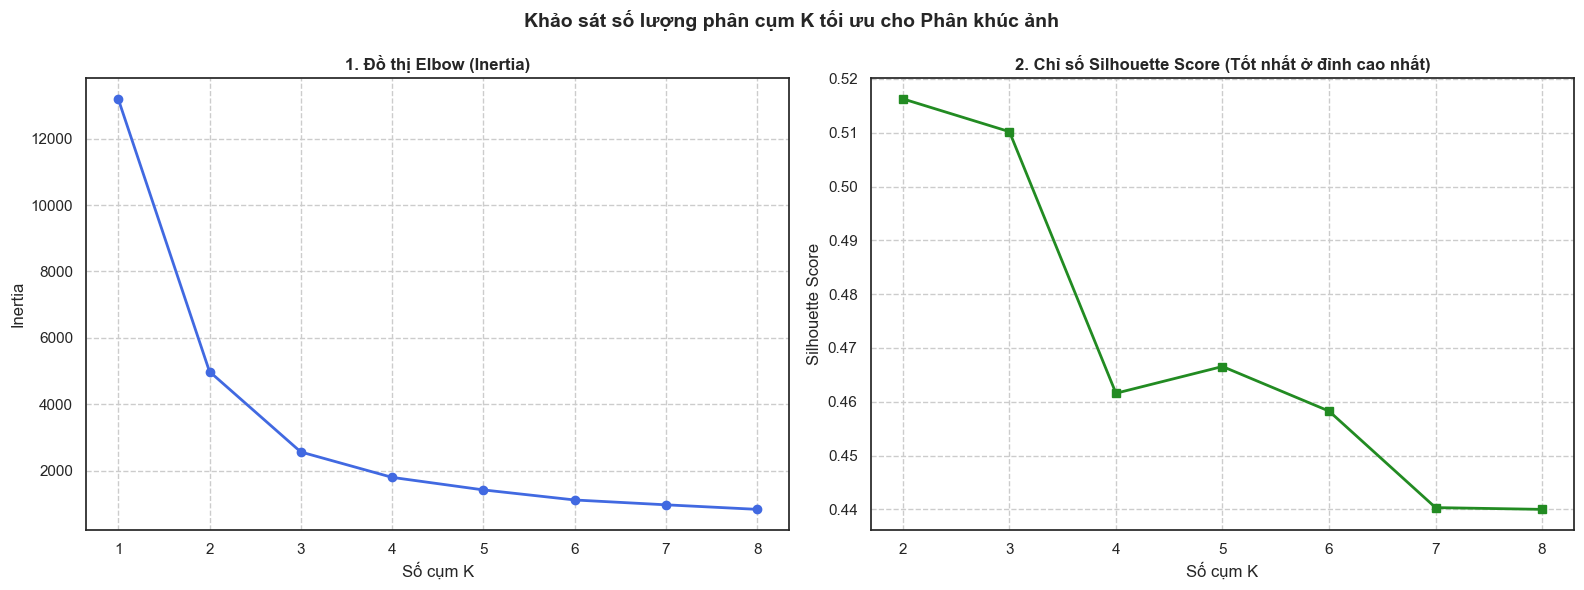
\includegraphics[width=0.95\textwidth]{figures/lab3_image_fig2.png}
    \caption{Elbow (Inertia) and Silhouette score curves on image pixels for K from 1 to 8.}
    \label{fig:lab3_seg_2}
\end{figure}
Figure~\ref{fig:lab3_seg_2} displays the elbow inflection point at $K=3$.

\subsubsection{Segmented Visualizations and Semantic Analysis}
The segmented images across color spaces are shown in Figure~\ref{fig:lab3_seg_3}.
\begin{figure}[H]
    \centering
    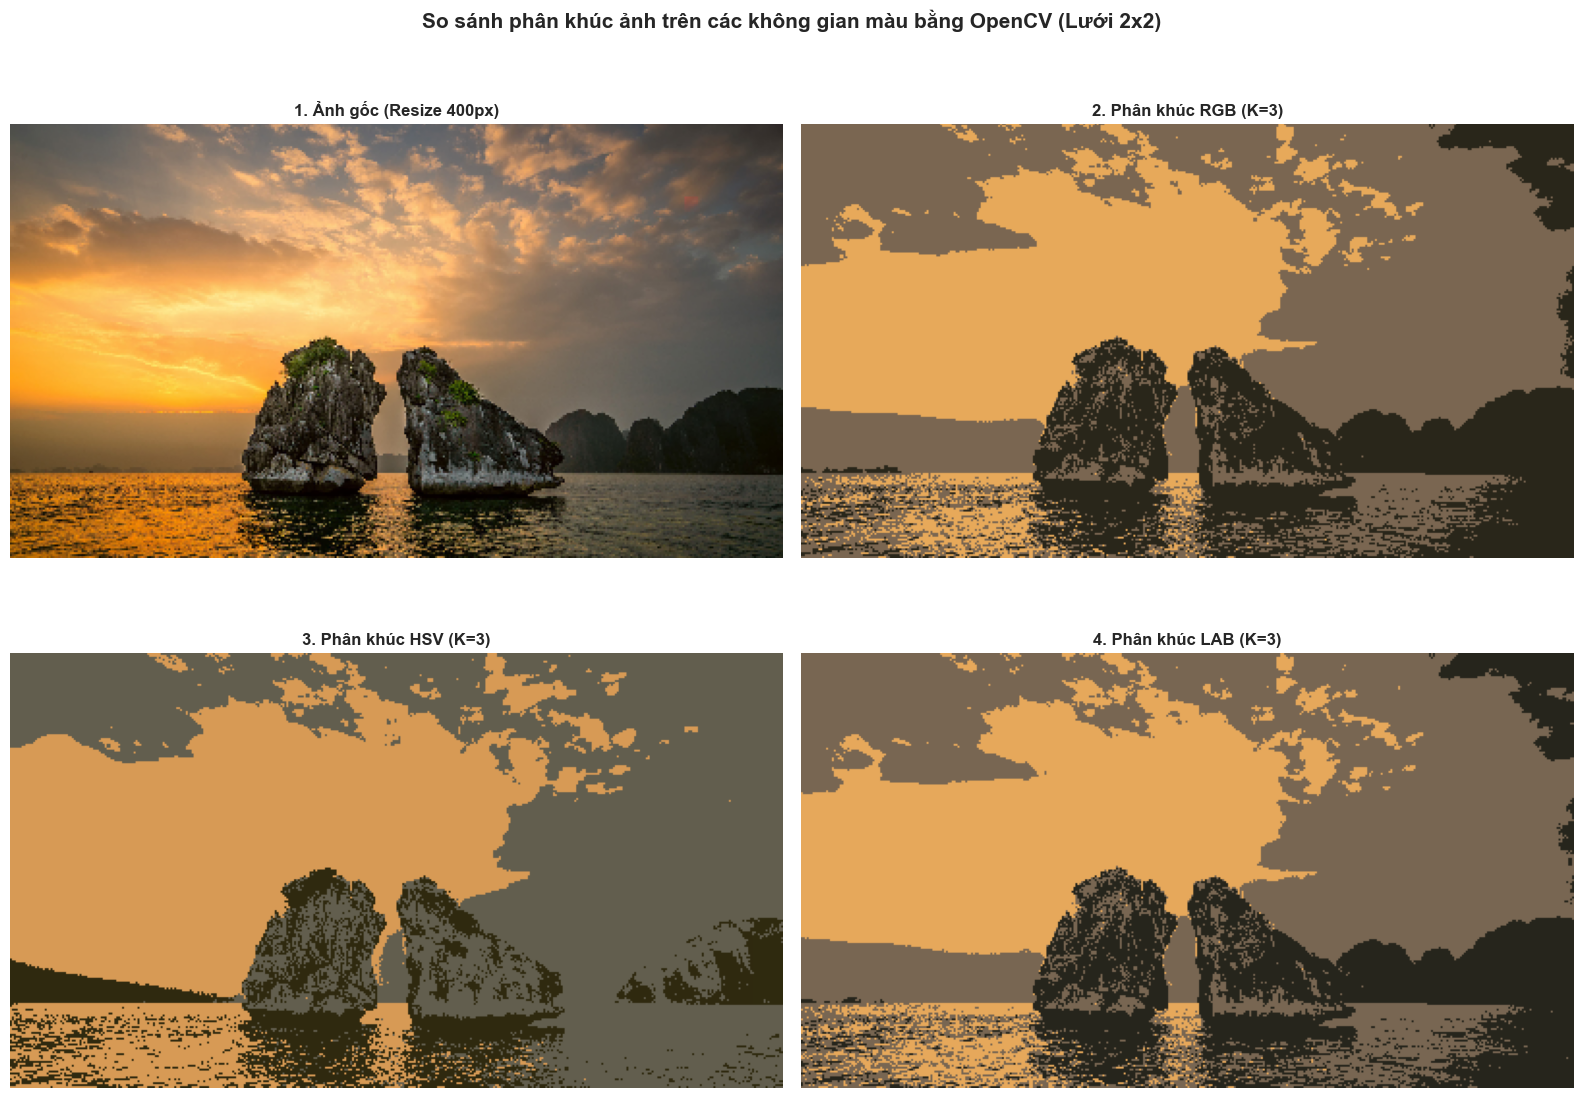
\includegraphics[width=0.95\textwidth]{figures/lab3_image_fig3.png}
    \caption{Visual segmentation results comparing RGB, HSV, and CIELAB color spaces at K=3.}
    \label{fig:lab3_seg_3}
\end{figure}
Figure~\ref{fig:lab3_seg_3} compares the segmentation results. The CIELAB segmentation (bottom-right) produces clean boundaries between the sky, water, and rocks. The RGB segmentation (top-right) shows noise in the water region, misclassifying shadowed waves as rock due to luminance variations.

To perform a semantic analysis, we analyze the centroids of the three clusters in the RGB model. The centroid coordinates are shown in Figure~\ref{fig:lab3_seg_4}.
\begin{figure}[H]
    \centering
    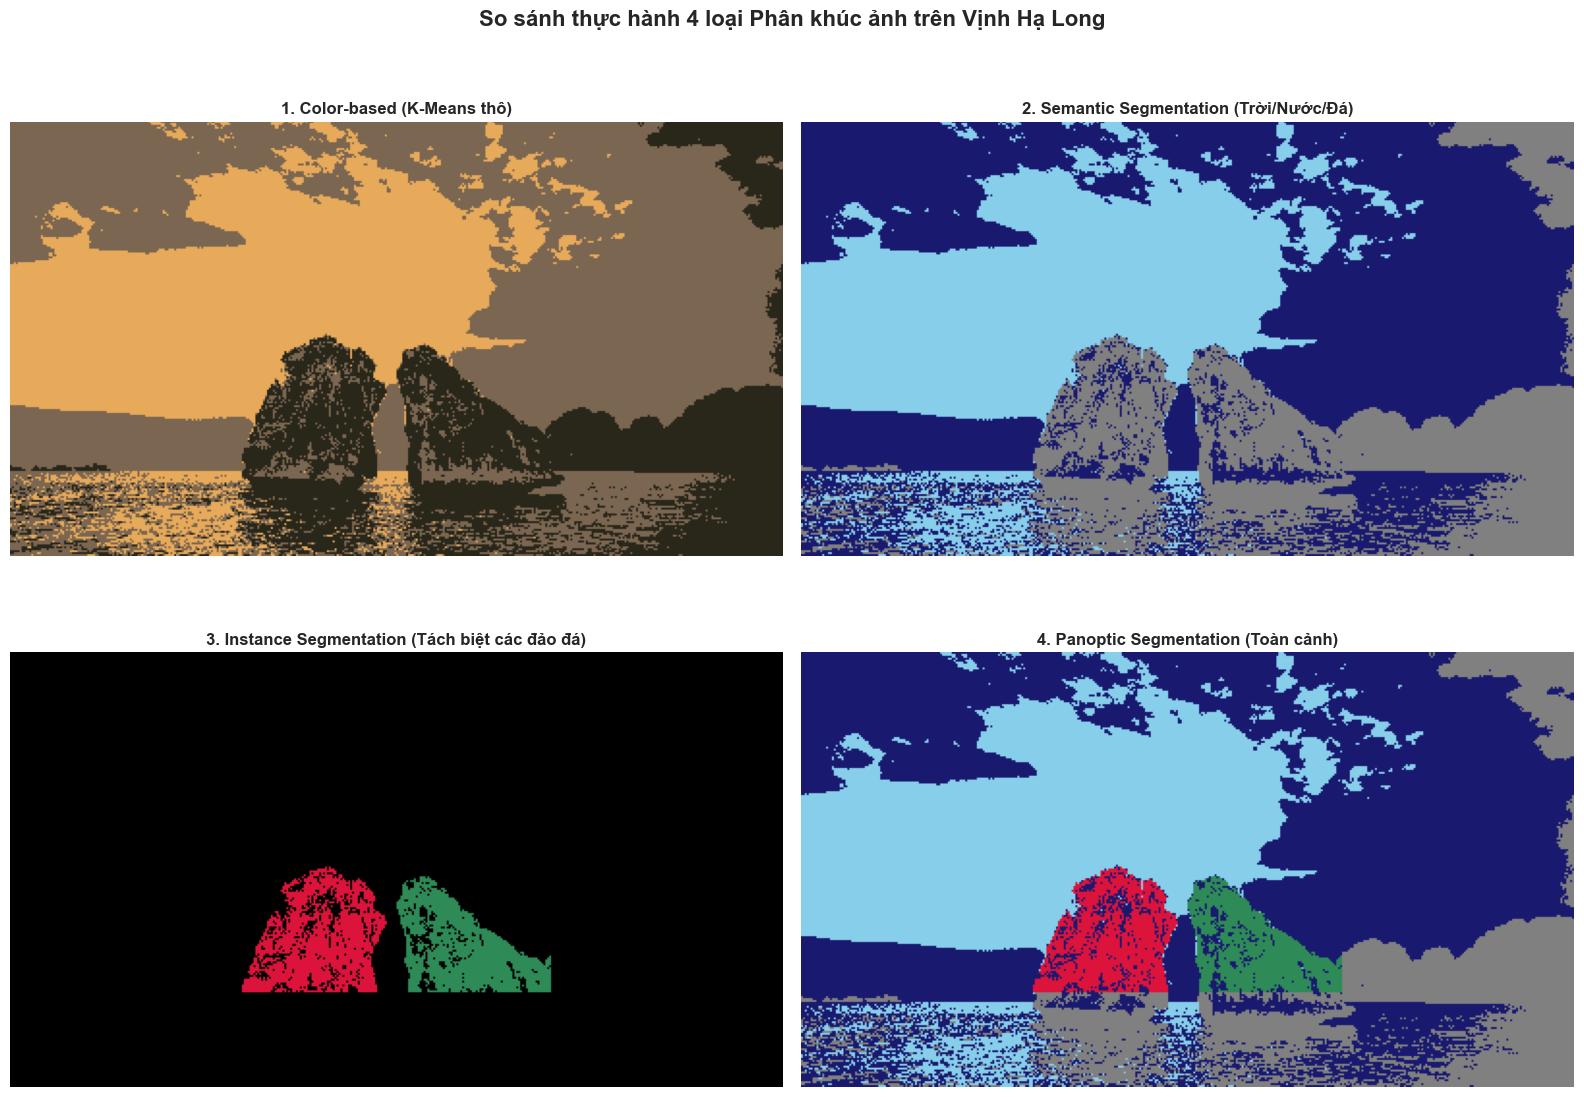
\includegraphics[width=0.95\textwidth]{figures/lab3_image_fig4.png}
    \caption{Centroid coordinate analysis showing the RGB color signatures of the sky, water, and rock clusters.}
    \label{fig:lab3_seg_4}
\end{figure}
Figure~\ref{fig:lab3_seg_4} displays the centroid values:
\begin{itemize}
    \item \textbf{Cluster 1 (Sky):} High blue-channel values, capturing the sky region.
    \item \textbf{Cluster 2 (Water):} Medium green and blue values, capturing the water surface.
    \item \textbf{Cluster 3 (Rocks):} Low overall values across all channels, capturing the dark rock formations.
\end{itemize}
This centroid analysis confirms that K-Means successfully partitions the image based on the three physical regions.


% ==========================================
% SECTION 4: LAB 4
% ==========================================
\newpage
\section{-- Lab 4 - California House Price Prediction using MLP}

This section details the empirical experiments, preprocessing scenarios, scratch and deep learning models, and comparative results of the house price regression task, based strictly on the project notebooks: \texttt{eda.ipynb}, \texttt{feature\_engineering.ipynb}, and \texttt{modeling\_kaggle.ipynb} inside the \texttt{lab4} workspace.

\subsection{Jupyter Notebook Step 1: Exploratory Data Analysis (EDA) \& Data Quality}
The exploratory phase investigates the distribution of housing price targets, feature correlations, geographical patterns, and isolates missing and outlier records.

\subsubsection{Dataset Context, Dimensions \& Initial Inspection}
The dataset utilized is the **California Housing Dataset**, which records demographic and structural indicators for 20,640 block groups in California based on the 1990 census. It contains 10 attributes: longitude, latitude, housing median age, total rooms, total bedrooms, population, households, median income, median house value (target), and ocean proximity. Predicting house values is a fundamental task for spatial economics, urban planning, and mortgage risk valuation.

The raw CSV file containing 20,640 records is loaded in the notebook:
\begin{verbatim}
Kich thuoc du lieu: 20640 dong, 10 cot
\end{verbatim}

The distributions of the target variable, median income, and ocean proximity are plotted in Figure~\ref{fig:lab4_eda_1}.
\begin{figure}[H]
    \centering
    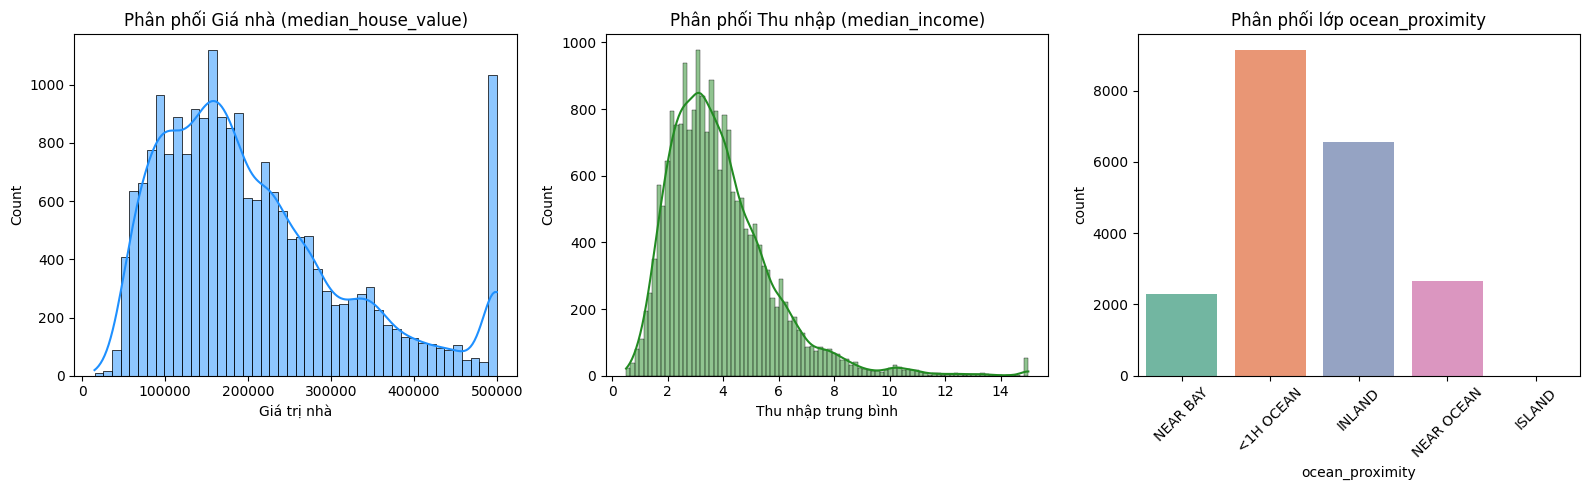
\includegraphics[width=0.95\textwidth]{figures/lab4_eda_fig1.png}
    \caption{Target Variable (median house value), Median Income, and Ocean Proximity distributions.}
    \label{fig:lab4_eda_1}
\end{figure}
Figure~\ref{fig:lab4_eda_1} reveals that \texttt{median\_house\_value} (left) displays a broad right-skewed profile but exhibits a sharp spike at \$500,001. This is a critical data anomaly representing an artificial upper cap: all homes valued above \$500,000 were grouped into this boundary bin. Median Income (center) is slightly right-skewed, peaking between \$2.0 and \$4.0 (tens of thousands of USD). Ocean Proximity (right) is dominated by the \texttt{<1H OCEAN} and \texttt{INLAND} classes, reflecting coastal population density.

\subsubsection{Correlation and Spatial Geographical Analysis}
The Pearson correlation heatmap of continuous features, along with scatter plots analyzing relationships, are visualized in Figures~\ref{fig:lab4_eda_2}, \ref{fig:lab4_eda_3}, and \ref{fig:lab4_eda_4}.
\begin{figure}[H]
    \centering
    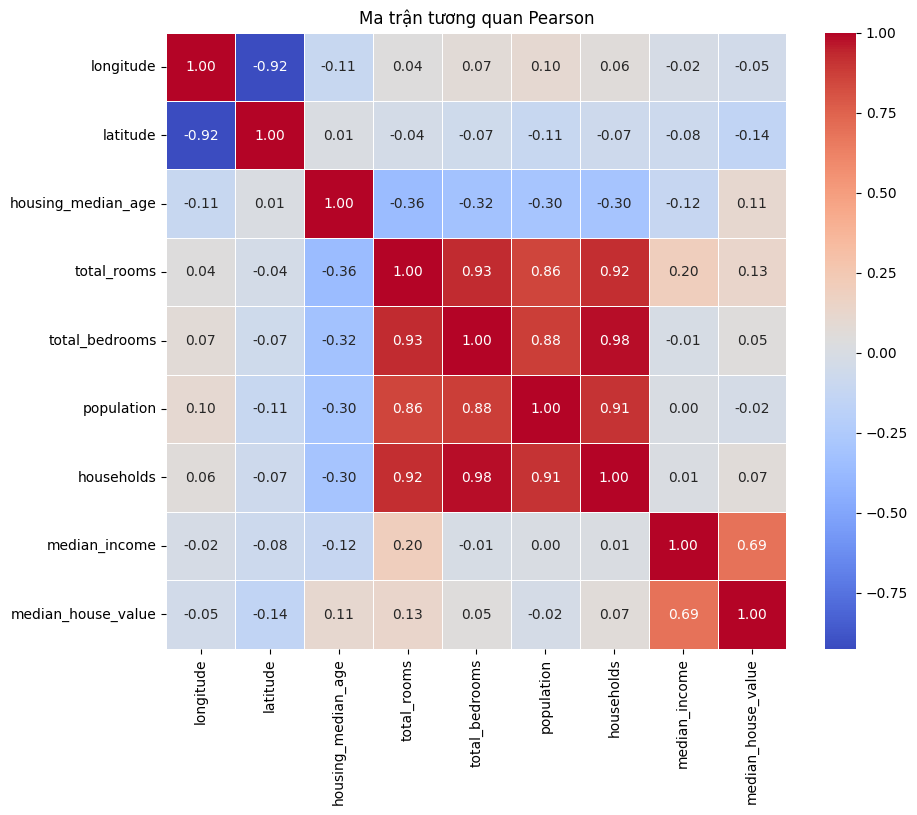
\includegraphics[width=0.95\textwidth]{figures/lab4_eda_fig2.png}
    \caption{Pearson correlation matrix heatmap of raw continuous features.}
    \label{fig:lab4_eda_2}
\end{figure}
As shown in Figure~\ref{fig:lab4_eda_2}, the feature showing the highest positive correlation with \texttt{median\_house\_value} is \texttt{median\_income} (r = 0.69). Scale features like rooms, bedrooms, population, and households show high inter-correlations (r $>$ 0.90), indicating strong multicollinearity.

\begin{figure}[H]
    \centering
    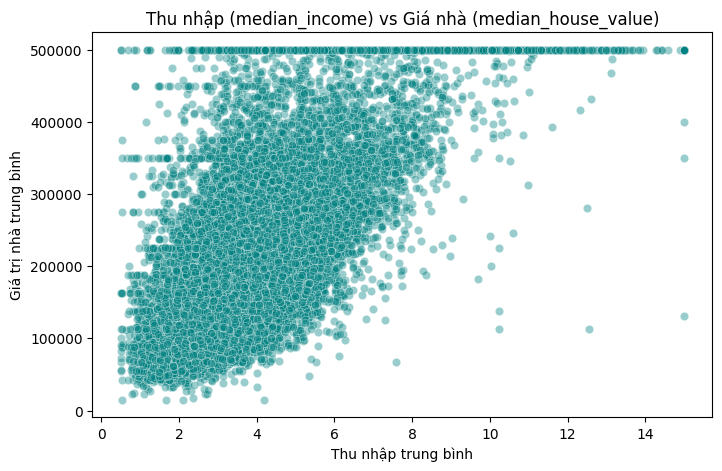
\includegraphics[width=0.95\textwidth]{figures/lab4_eda_fig3.png}
    \caption{Scatter plot of Median Income vs. Median House Value.}
    \label{fig:lab4_eda_3}
\end{figure}
Figure~\ref{fig:lab4_eda_3} plots Income vs. House Value. It displays a clear positive trend, but confirms the sharp ceiling effect at the \$500,001 capping threshold, where points form a solid horizontal line at the top.

\begin{figure}[H]
    \centering
    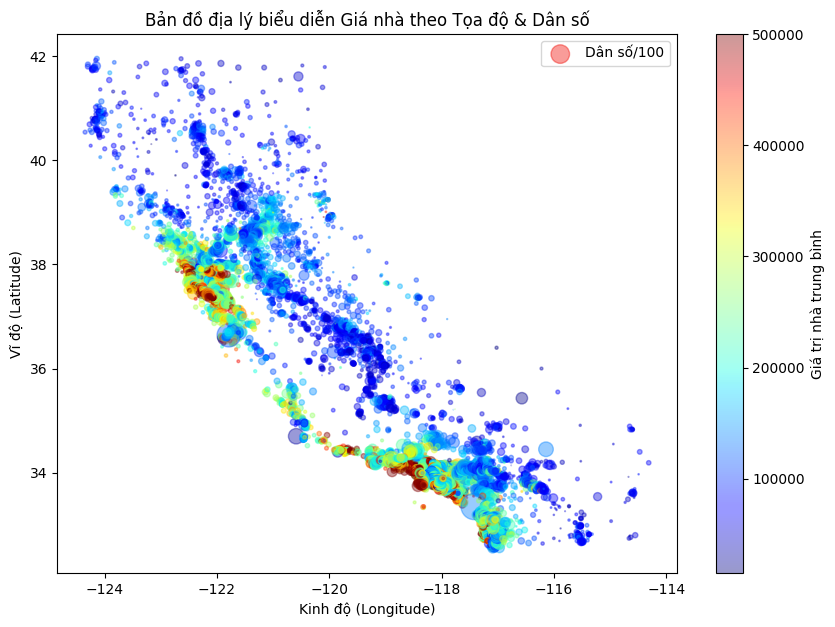
\includegraphics[width=0.95\textwidth]{figures/lab4_eda_fig4.png}
    \caption{Geographical scatter plot mapping latitude and longitude to median house values and population density.}
    \label{fig:lab4_eda_4}
\end{figure}
Figure~\ref{fig:lab4_eda_4} displays the geographical map of California housing. High-value blocks (red dots) are concentrated along the coastline and surrounding major metropolitan areas (San Francisco and Los Angeles), demonstrating that spatial coordinates (latitude and longitude) are strong non-linear predictors of house values.

The distribution of house value across ocean proximity categories is shown in Figure~\ref{fig:lab4_eda_5}.
\begin{figure}[H]
    \centering
    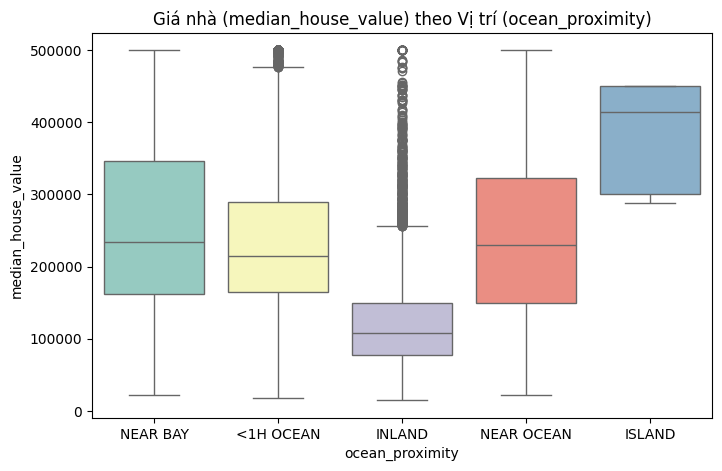
\includegraphics[width=0.95\textwidth]{figures/lab4_eda_fig5.png}
    \caption{Box plots comparing house values across different ocean proximity regions.}
    \label{fig:lab4_eda_5}
\end{figure}
Figure~\ref{fig:lab4_eda_5} confirms that houses located \texttt{INLAND} have significantly lower median values compared to coastal categories, making proximity a vital categorical feature.

\subsubsection{Data Quality Assessment}
We check for duplicates and missing values in the dataset.
The data completeness is plotted in Figure~\ref{fig:lab4_eda_6}.
\begin{figure}[H]
    \centering
    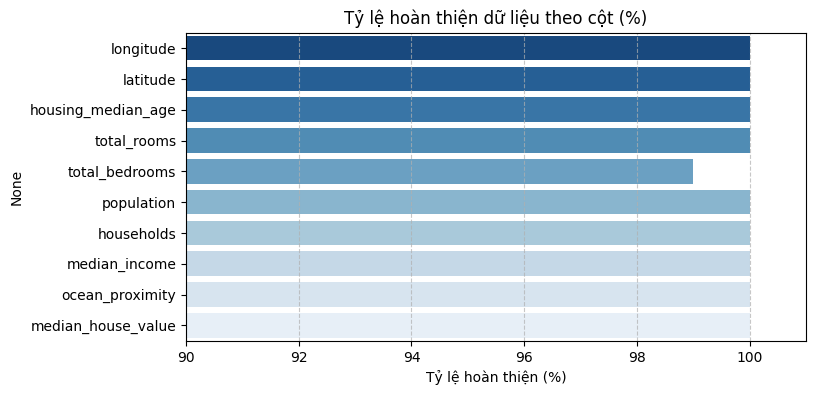
\includegraphics[width=0.95\textwidth]{figures/lab4_eda_fig6.png}
    \caption{Bar chart displaying the data completeness percentage across all 10 columns.}
    \label{fig:lab4_eda_6}
\end{figure}
Figure~\ref{fig:lab4_eda_6} shows that data completeness is 100\% for nine columns, but drops slightly to 99.00\% for \texttt{total\_bedrooms}, which has **207 missing values**. No duplicate rows exist.

\subsection{Jupyter Notebook Step 2: Feature Engineering \& Preprocessing}
This step prepares the training matrices and sets up four comparative feature scenarios.

\subsubsection{Preprocessing Flow of Thinking}
The preprocessing workflow is designed as follows:
\begin{enumerate}
    \item \textbf{Missing Data Imputation:}\mbox{}\\ The 207 missing values in \texttt{total\_bedrooms} are imputed using the **Median** of the training set (435.0), and a binary missing indicator column is added. Imputing with the median prevents bias from skewed distributions.
    \item \textbf{Outlier Handling \& Log Transformation:}\mbox{}\\ Scale variables (\texttt{total\_rooms}, \texttt{total\_bedrooms}, \texttt{population}, \texttt{households}, \texttt{median\_income}) are heavily right-skewed. We apply log1p transformation:
        \[
        x\_{\text{log}} = \log(x + 1)
        \]
        to normalize the distributions. Outliers are capped based on training set IQR boundaries to prevent extreme values from distorting gradients.
    \item \textbf{Categorical Encoding:}\mbox{}\\ The nominal feature \texttt{ocean\_proximity} is One-Hot encoded, yielding five binary columns (e.g. \texttt{ocean\_proximity\_INLAND}).
\end{enumerate}

\subsubsection{Feature Set Scenarios}
To evaluate the impact of multicollinearity and spatial aggregation, the features are prepared in four configurations:
\begin{itemize}
    \item \textbf{PA1 (Base Features):}\mbox{}\\ Keeps all original features scaled using \texttt{StandardScaler}. Yields a train shape of $(16512, 13)$ features.
    \item \textbf{PA2 (Reduced Features):}\mbox{}\\ Drops \texttt{total\_bedrooms} and \texttt{households} to reduce multicollinearity, and adds a spatial interaction feature \texttt{coords\_sum} (\texttt{latitude} + \texttt{longitude}). Yields $(16512, 10)$ features.
    \item \textbf{PA3\_A (Mean Aggregation):}\mbox{}\\ Combines collinear columns by taking their average (e.g. mean of rooms and bedrooms), plus \texttt{coords\_sum}. Yields $(16512, 10)$ features.
    \item \textbf{PA3\_B (PCA Aggregation):}\mbox{}\\ Aggregates the collinear room and household columns using 1D PCA (PC1 explains 95.8\% variance), plus \texttt{coords\_sum}. Yields $(16512, 9)$ features.
\end{itemize}

A summary of all configurations is presented in Table~\ref{tab:summary_fe_lab4}.
\begin{table}[H]
\centering
\caption{Lab 4 Scenario Configurations and Features Summary}
\label{tab:summary_fe_lab4}
\begin{tabular}{lcp{9.5cm}}
\toprule
\textbf{Scenario} & \textbf{Number of Features} & \textbf{Feature Names} \\
\midrule
PA1 (Base) & 13 & \texttt{longitude}, \texttt{latitude}, \texttt{housing\_median\_age}, \texttt{total\_rooms\_log}, \texttt{total\_bedrooms\_log}, \texttt{population\_log}, \texttt{households\_log}, \texttt{median\_income\_log}, \texttt{5 $\times$ ocean\_proximity\_OHE} \\
PA2 (Reduced) & 10 & \texttt{housing\_median\_age}, \texttt{total\_rooms\_log}, \texttt{population\_log}, \texttt{median\_income\_log}, \texttt{coords\_sum}, \texttt{5 $\times$ ocean\_proximity\_OHE} \\
PA3\_A (Mean) & 10 & \texttt{housing\_median\_age}, \texttt{median\_income\_log}, \texttt{rooms\_bedrooms\_combined}, \texttt{pop\_hhold\_combined}, \texttt{coords\_sum}, \texttt{5 $\times$ ocean\_proximity\_OHE} \\
PA3\_B (PCA) & 9 & \texttt{housing\_median\_age}, \texttt{median\_income\_log}, \texttt{pca\_1d}, \texttt{coords\_sum}, \texttt{5 $\times$ ocean\_proximity\_OHE} \\
\bottomrule
\end{tabular}
\end{table}

\pagebreak
The Pearson correlation heatmaps for the four scenarios are visualized in Figures~\ref{fig:lab4_fe_1} to \ref{fig:lab4_fe_4}.
\begin{figure}[H]
    \centering
    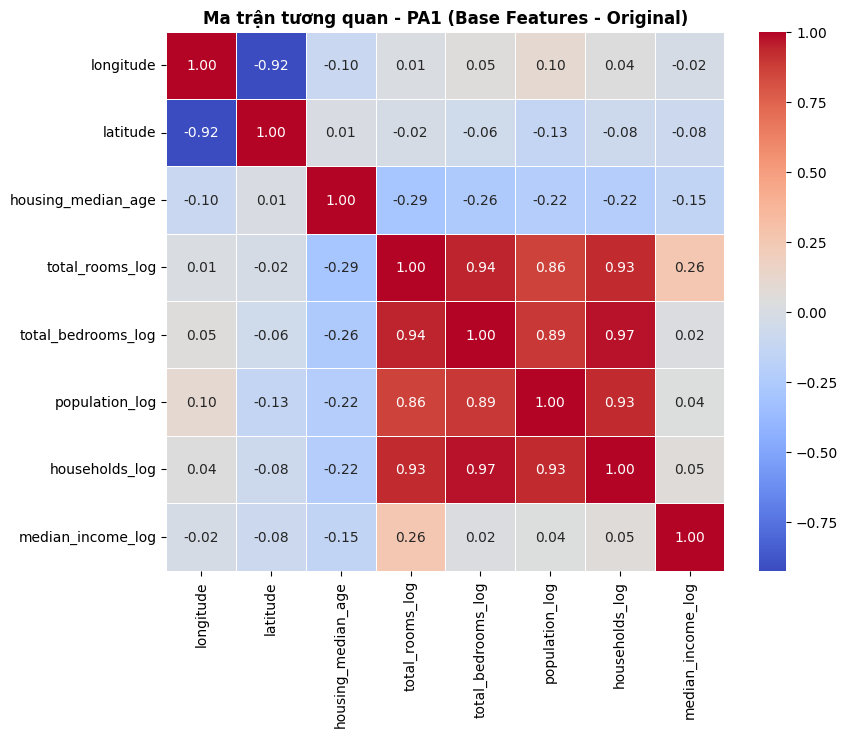
\includegraphics[width=0.95\textwidth]{figures/lab4_feature_fig1.png}
    \caption{Pearson correlation matrix heatmap for Scenario PA1 (Base Features).}
    \label{fig:lab4_fe_1}
\end{figure}
Figure~\ref{fig:lab4_fe_1} shows high correlation coefficients (r $>$ 0.90) among rooms, bedrooms, and households.

\begin{figure}[H]
    \centering
    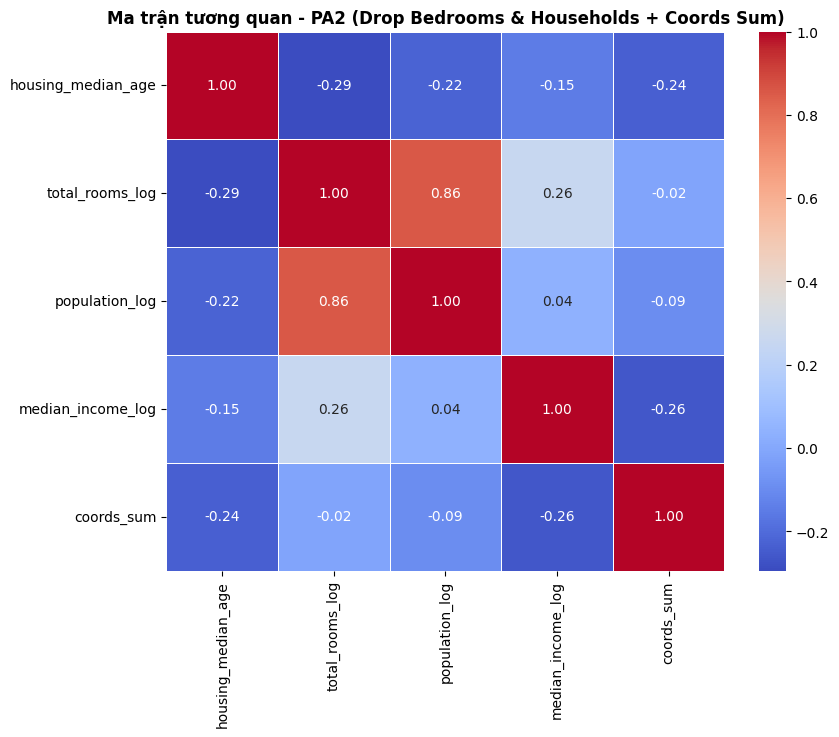
\includegraphics[width=0.95\textwidth]{figures/lab4_feature_fig2.png}
    \caption{Pearson correlation matrix heatmap for Scenario PA2 (Reduced Features).}
    \label{fig:lab4_fe_2}
\end{figure}
Figure~\ref{fig:lab4_fe_2} shows that dropping bedrooms and households successfully reduces multicollinearity, bringing all correlation coefficients under 0.80.

\begin{figure}[H]
    \centering
    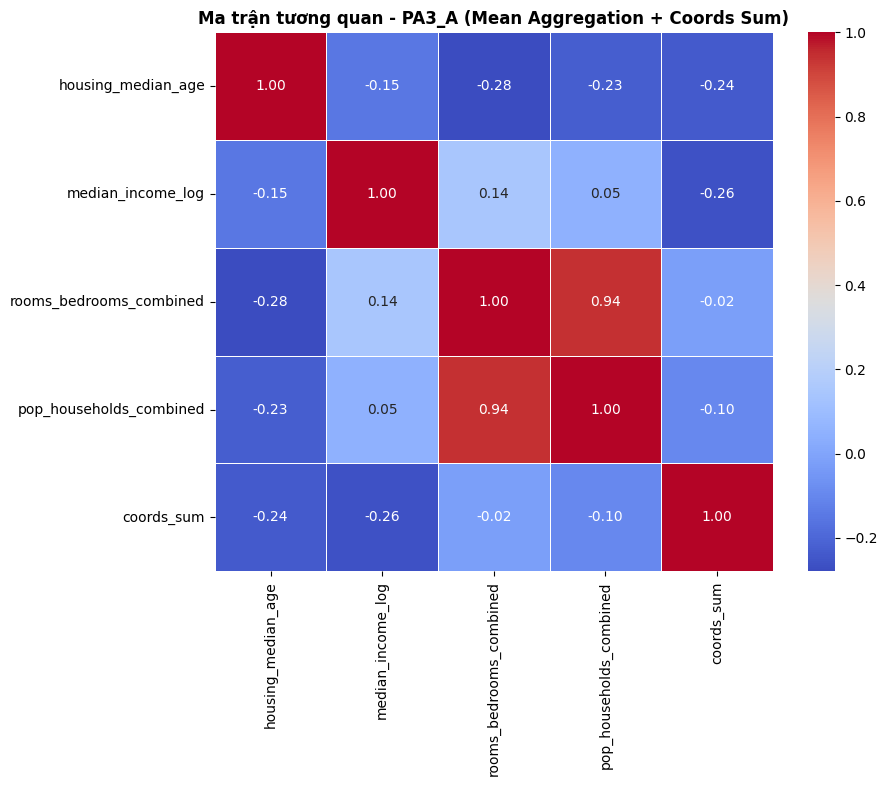
\includegraphics[width=0.95\textwidth]{figures/lab4_feature_fig3.png}
    \caption{Pearson correlation matrix heatmap for Scenario PA3\_A (Mean Aggregation).}
    \label{fig:lab4_fe_3}
\end{figure}
Figure~\ref{fig:lab4_fe_3} shows that mean aggregation retains structural scale variance while maintaining low multicollinearity.

\begin{figure}[H]
    \centering
    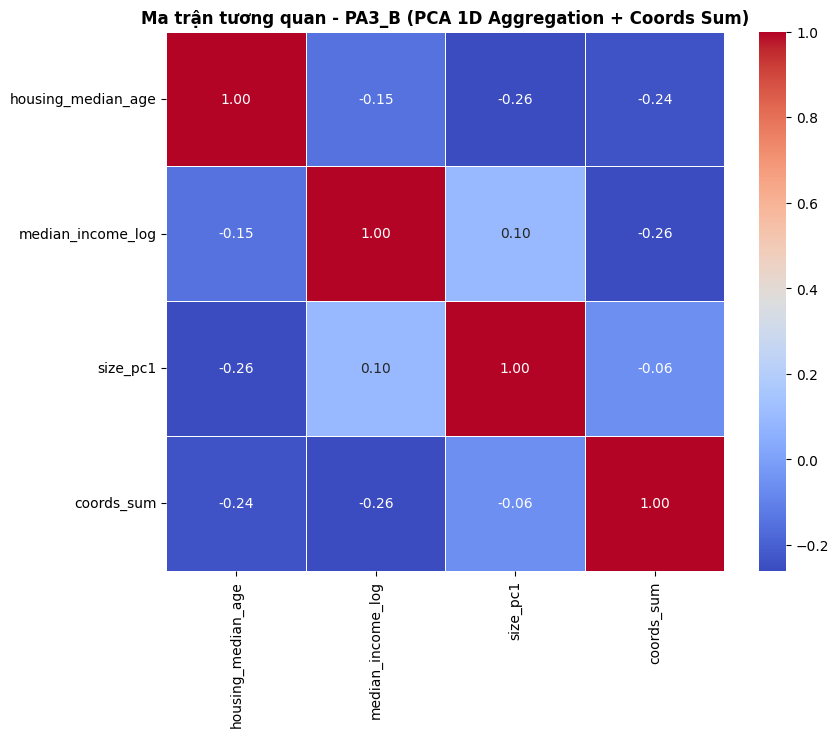
\includegraphics[width=0.95\textwidth]{figures/lab4_feature_fig4.png}
    \caption{Pearson correlation matrix heatmap for Scenario PA3\_B (PCA Aggregation).}
    \label{fig:lab4_fe_4}
\end{figure}
Figure~\ref{fig:lab4_fe_4} displays the correlation heatmap of the PCA scenario, demonstrating clean, decorrelated features.

\subsection{Jupyter Notebook Step 3: Modeling \& Performance Comparison}
We compare three regression models: a custom Linear Regression Scratch model, a Random Forest, and a PyTorch Multi-Layer Perceptron (MLP).

\subsubsection{Model Architectures}
\begin{itemize}
    \item \textbf{LR Scratch:}\mbox{}\\ Implements multivariate linear regression optimized using subgradient descent on Mean Squared Error (MSE) loss:
        \[
        L = \frac{1}{N} \sum\_{i=1}^{N} \left( y\_i - (X\_i \cdot w + b) \right)^2
        \]
    \item \textbf{Random Forest:}\mbox{}\\ An ensemble of decision trees trained to output the average prediction.
    \item \textbf{MLP (PyTorch Neural Network):}\mbox{}\\ A feed-forward deep network implemented in PyTorch. The architecture contains:
        \begin{itemize}
            \item Input layer mapping to a 128-neuron hidden layer, followed by Batch Normalization, ReLU activation, and a 20\% Dropout layer.
            \item Second hidden layer of 64 neurons, followed by Batch Normalization, ReLU, and 20\% Dropout.
            \item Output layer of 1 neuron.
        \end{itemize}
        The network is optimized using the Adam optimizer with a learning rate of 0.01 and MSE loss, trained over 100 epochs with batch size 128.
\end{itemize}

\paragraph{Mathematical Code Loops}
The core fitting optimization loop from our Linear Regression scratch implementation is shown in Listing 4.
\begin{lstlisting}[language=Python, caption=Linear Regression Scratch Core Fitting Loop]
def fit(self, X, y):
    n_samples, n_features = X.shape
    self.weights = np.zeros(n_features)
    self.bias = 0.0
    for epoch in range(self.epochs):
        # Generate model predictions
        y_pred = X.dot(self.weights) + self.bias
        # Compute analytical gradients of MSE loss
        dw = (2.0 / n_samples) * X.T.dot(y_pred - y)
        db = (2.0 / n_samples) * np.sum(y_pred - y)
        # Update weights and bias
        self.weights -= self.lr * dw
        self.bias -= self.lr * db
\end{lstlisting}

\paragraph{Random Forest and MLP Custom Implementations}
To illustrate the modeling process for the other algorithms utilized in the California Housing experiments, Listing 5 details the custom RandomForestRegressorScratch model class and bootstrap fitting loop, and Listing 6 shows the complete custom PyTorch MLPRegressor class and dataset representation.

\begin{lstlisting}[language=Python, caption=Custom RandomForestRegressorScratch Fitting Loop]
class RandomForestRegressorScratch:
    def __init__(self, n_estimators=30, max_depth=10, min_samples_split=10, max_features='sqrt', random_state=42):
        self.n_estimators = n_estimators
        self.max_depth = max_depth
        self.min_samples_split = min_samples_split
        self.max_features = max_features
        self.random_state = random_state
        self.trees = []
        self.loss_hist = []

    def fit(self, X, y):
        if self.random_state is not None:
            np.random.seed(self.random_state)
            
        X_arr = np.asarray(X)
        y_arr = np.asarray(y).ravel()
        n_samples = X_arr.shape[0]
        
        self.trees = []
        preds = np.zeros((n_samples, self.n_estimators))
        
        for i in range(self.n_estimators):
            boot_idx = np.random.choice(n_samples, n_samples, replace=True)
            X_boot, y_boot = X_arr[boot_idx], y_arr[boot_idx]
            
            tree = DecisionTreeRegressorScratch(
                max_depth=self.max_depth,
                min_samples_split=self.min_samples_split,
                max_features=self.max_features
            )
            tree.fit(X_boot, y_boot)
            self.trees.append(tree)
            
            preds[:, i] = tree.predict(X_arr).ravel()
            cum_pred = np.mean(preds[:, :i+1], axis=1)
            mse = float(np.mean((cum_pred - y_arr)**2))
            self.loss_hist.append(mse)
            
        return self

    def predict(self, X):
        X_arr = np.asarray(X)
        tree_preds = np.column_stack([tree.predict(X_arr).ravel() for tree in self.trees])
        return np.mean(tree_preds, axis=1).reshape(-1, 1)
\end{lstlisting}

\begin{lstlisting}[language=Python, caption=Custom PyTorch MLPRegressor Class and Dataset]
class HouseDataset(Dataset):
    def __init__(self, X, y):
        self.X = torch.tensor(X, dtype=torch.float32)
        self.y = torch.tensor(y, dtype=torch.float32)
    def __len__(self): return len(self.X)
    def __getitem__(self, i): return self.X[i], self.y[i]

class MLPRegressor(nn.Module):
    def __init__(self, in_dim):
        super().__init__()
        self.net = nn.Sequential( 
            nn.Linear(in_dim, 128), nn.BatchNorm1d(128), nn.ReLU(),
            nn.Dropout(0.2),
            nn.Linear(128, 64),  nn.BatchNorm1d(64),  nn.ReLU(),
            nn.Dropout(0.1),
            nn.Linear(64, 32),   nn.ReLU(),
            nn.Linear(32, 1)
        )
    def forward(self, x): return self.net(x)
\end{lstlisting}

\subsubsection{Validation Results and Discussion}
The performance metrics across the 4 scenarios and 3 models are summarized in Table~\ref{tab:lab4_comparison}.
\begin{table}[H]
\centering
\caption{Lab 4 Final Scenario Comparison Results Table}
\label{tab:lab4_comparison}
\resizebox{\textwidth}{!}{
\begin{tabular}{llcccccc}
\toprule
\textbf{Scenario} & \textbf{Model} & \textbf{MAE (USD)} & \textbf{RMSE (USD)} & \textbf{MAPE (\%)} & \textbf{R² Score} & \textbf{Train (ms)} & \textbf{Inf (ms)} \\
\midrule
PA1 (Base Features) & LR Scratch & 54,428 & 73,041 & 32.16\% & 0.5929 & 139 & 0.2 \\
PA1 (Base Features) & Random Forest & 38,837 & 55,906 & 22.32\% & 0.7615 & 23,177 & 193.2 \\
PA1 (Base Features) & MLP & \textbf{34,110} & \textbf{51,193} & \textbf{18.87\%} & \textbf{0.8000} & 38,678 & 1.1 \\
\midrule
PA2 (Reduced) & LR Scratch & 55,388 & 73,792 & 32.68\% & 0.5845 & 128 & 0.3 \\
PA2 (Reduced) & Random Forest & 43,161 & 61,837 & 25.01\% & 0.7082 & 19,498 & 179.9 \\
PA2 (Reduced) & MLP & \textbf{38,654} & \textbf{56,690} & \textbf{22.12\%} & \textbf{0.7547} & 38,464 & 1.2 \\
\midrule
PA3\_A (Mean Agg) & LR Scratch & 55,948 & 74,713 & 32.81\% & 0.5740 & 124 & 0.2 \\
PA3\_A (Mean Agg) & Random Forest & 44,123 & 62,535 & 25.67\% & 0.7016 & 18,391 & 178.0 \\
PA3\_A (Mean Agg) & MLP & \textbf{39,556} & \textbf{57,743} & \textbf{22.68\%} & \textbf{0.7456} & 38,631 & 1.1 \\
\midrule
PA3\_B (PCA Agg) & LR Scratch & 57,363 & 76,568 & 33.39\% & 0.5526 & 115 & 0.3 \\
PA3\_B (PCA Agg) & Random Forest & 45,252 & 64,151 & 26.36\% & 0.6859 & 14,594 & 171.5 \\
PA3\_B (PCA Agg) & MLP & \textbf{43,611} & \textbf{63,132} & \textbf{24.40\%} & \textbf{0.6958} & 38,349 & 1.0 \\
\bottomrule
\end{tabular}
}
\end{table}

Analyzing Table~\ref{tab:lab4_comparison}, we observe:
\begin{itemize}
    \item \textbf{Optimal Configuration:} The PyTorch MLP model under Scenario PA1 (Base Features) achieves the highest predictive accuracy, peaking at an $R^2$ score of **80.00\%** (80.00\% variance explained), an MAE of 34,110 USD, and a MAPE of 18.87\%.
    \item \textbf{Deep Learning vs. Linear Baseline:} The MLP significantly outperforms the Linear Regression Scratch baseline ($R^2 = 59.29\%$). This is because housing values exhibit strong non-linear spatial relationships (e.g. proximity to coastlines and metropolitan centers), which linear models cannot capture but deep neural networks with non-linear activation functions (ReLU) can learn.
    \item \textbf{Dimensionality Reduction Impact:} Dropping features (PA2) or aggregating them (PA3\_A, PA3\_B) consistently reduces model performance. For the MLP, R2 drops from 80.00\% (PA1) to 75.47\% (PA2) and 69.58\% (PA3\_B). This demonstrates that despite collinearity, retaining raw features is critical for deep networks, which can automatically handle multicollinearity via hidden weight adjustments.
    \item \textbf{Inference Speed Trade-off:} The MLP model displays extremely fast inference times (1.1 ms) compared to the Random Forest ensemble (193.2 ms), making it highly suitable for real-world deployment.
\end{itemize}

The loss convergence curves for the optimal scenario (PA1) are plotted in Figure~\ref{fig:lab4_mod_1}.
\begin{figure}[H]
    \centering
    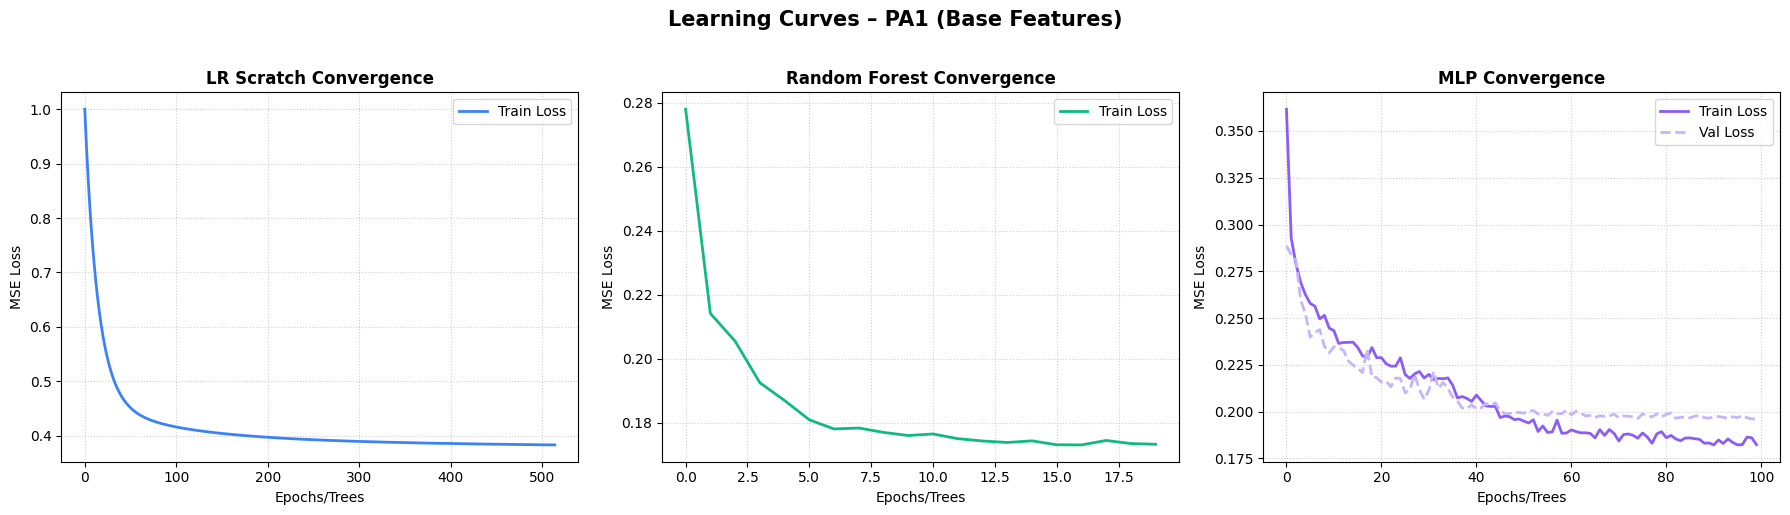
\includegraphics[width=0.95\textwidth]{figures/lab4_modeling_fig1.png}
    \caption{Loss convergence curves for LR Scratch, Random Forest, and MLP under Scenario PA1.}
    \label{fig:lab4_mod_1}
\end{figure}
Figure~\ref{fig:lab4_mod_1} plots convergence. The MLP curve displays a smooth validation loss decrease, stabilizing around epoch 80 with no signs of overfitting, proving the effectiveness of the Batch Normalization and Dropout regularizers.

The bar charts comparing validation metrics are shown in Figure~\ref{fig:lab4_mod_2}.
\begin{figure}[H]
    \centering
    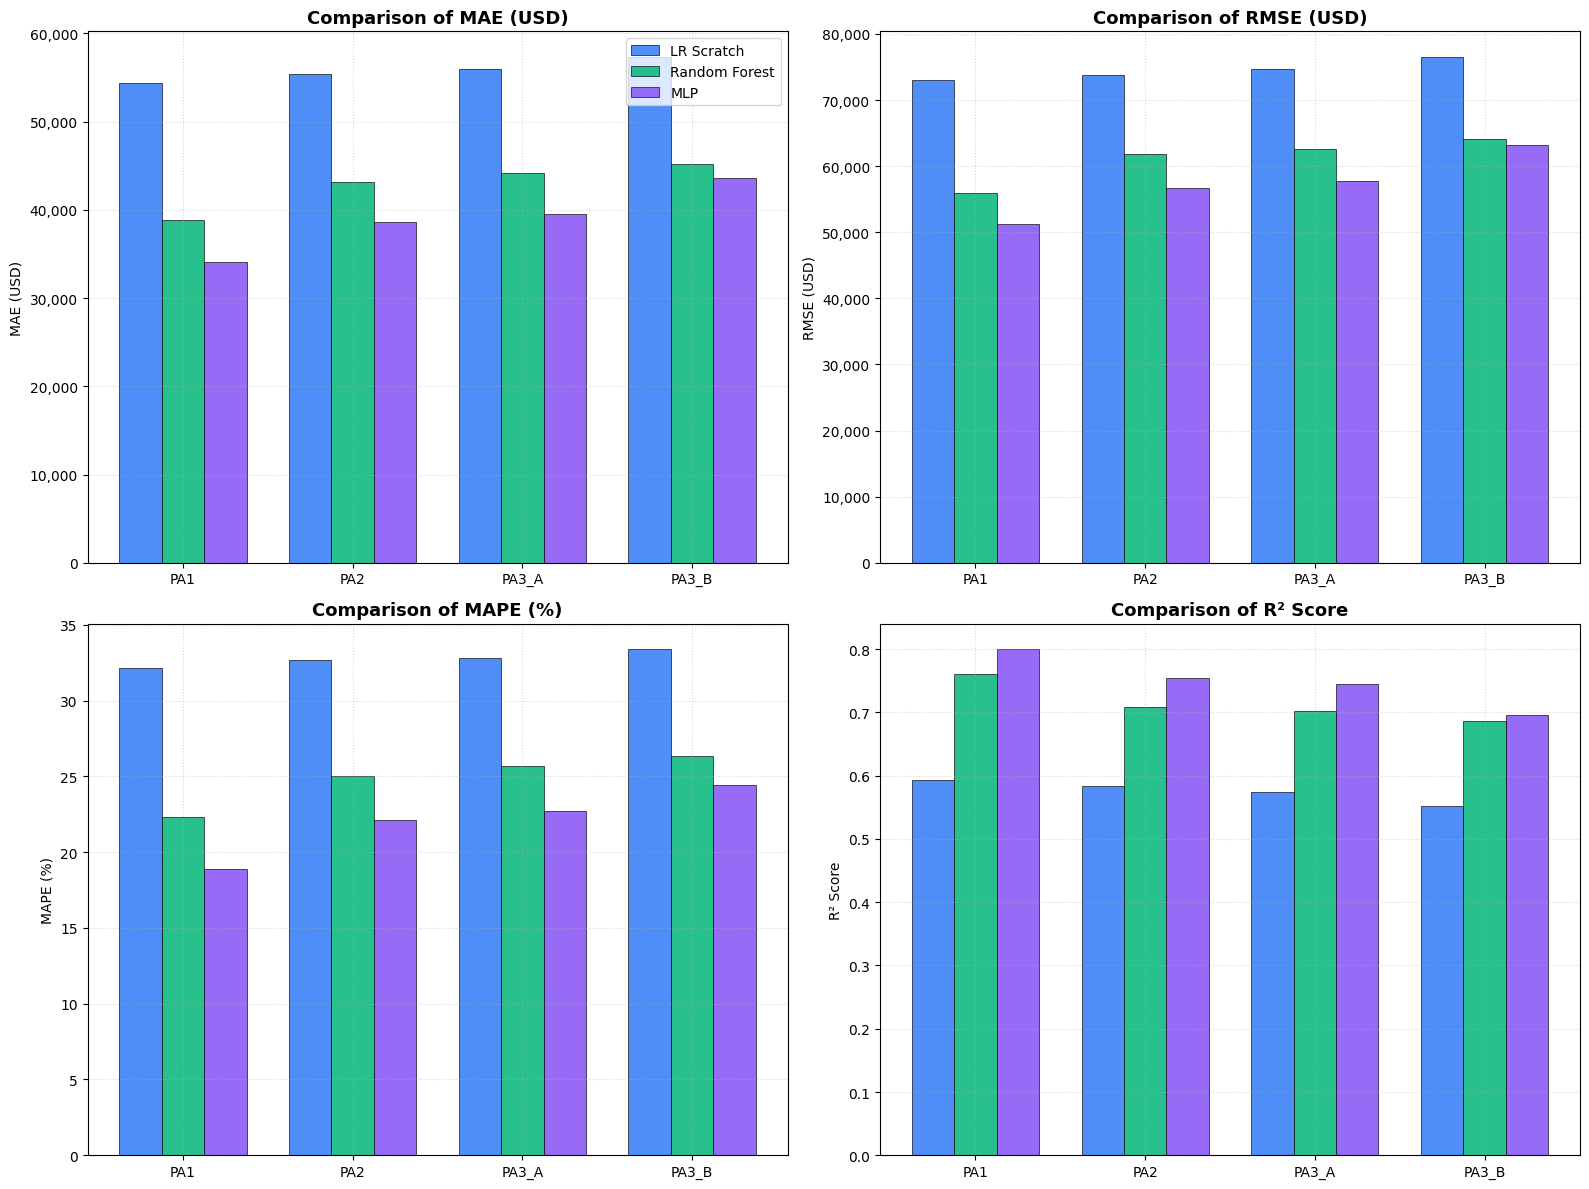
\includegraphics[width=0.95\textwidth]{figures/lab4_modeling_fig2.png}
    \caption{Bar charts comparing MAE, RMSE, MAPE, and R2 across models and scenarios.}
    \label{fig:lab4_mod_2}
\end{figure}
Figure~\ref{fig:lab4_mod_2} displays metric comparisons.

The predicted vs. actual house value scatter plots are shown in Figure~\ref{fig:lab4_mod_3}.
\begin{figure}[H]
    \centering
    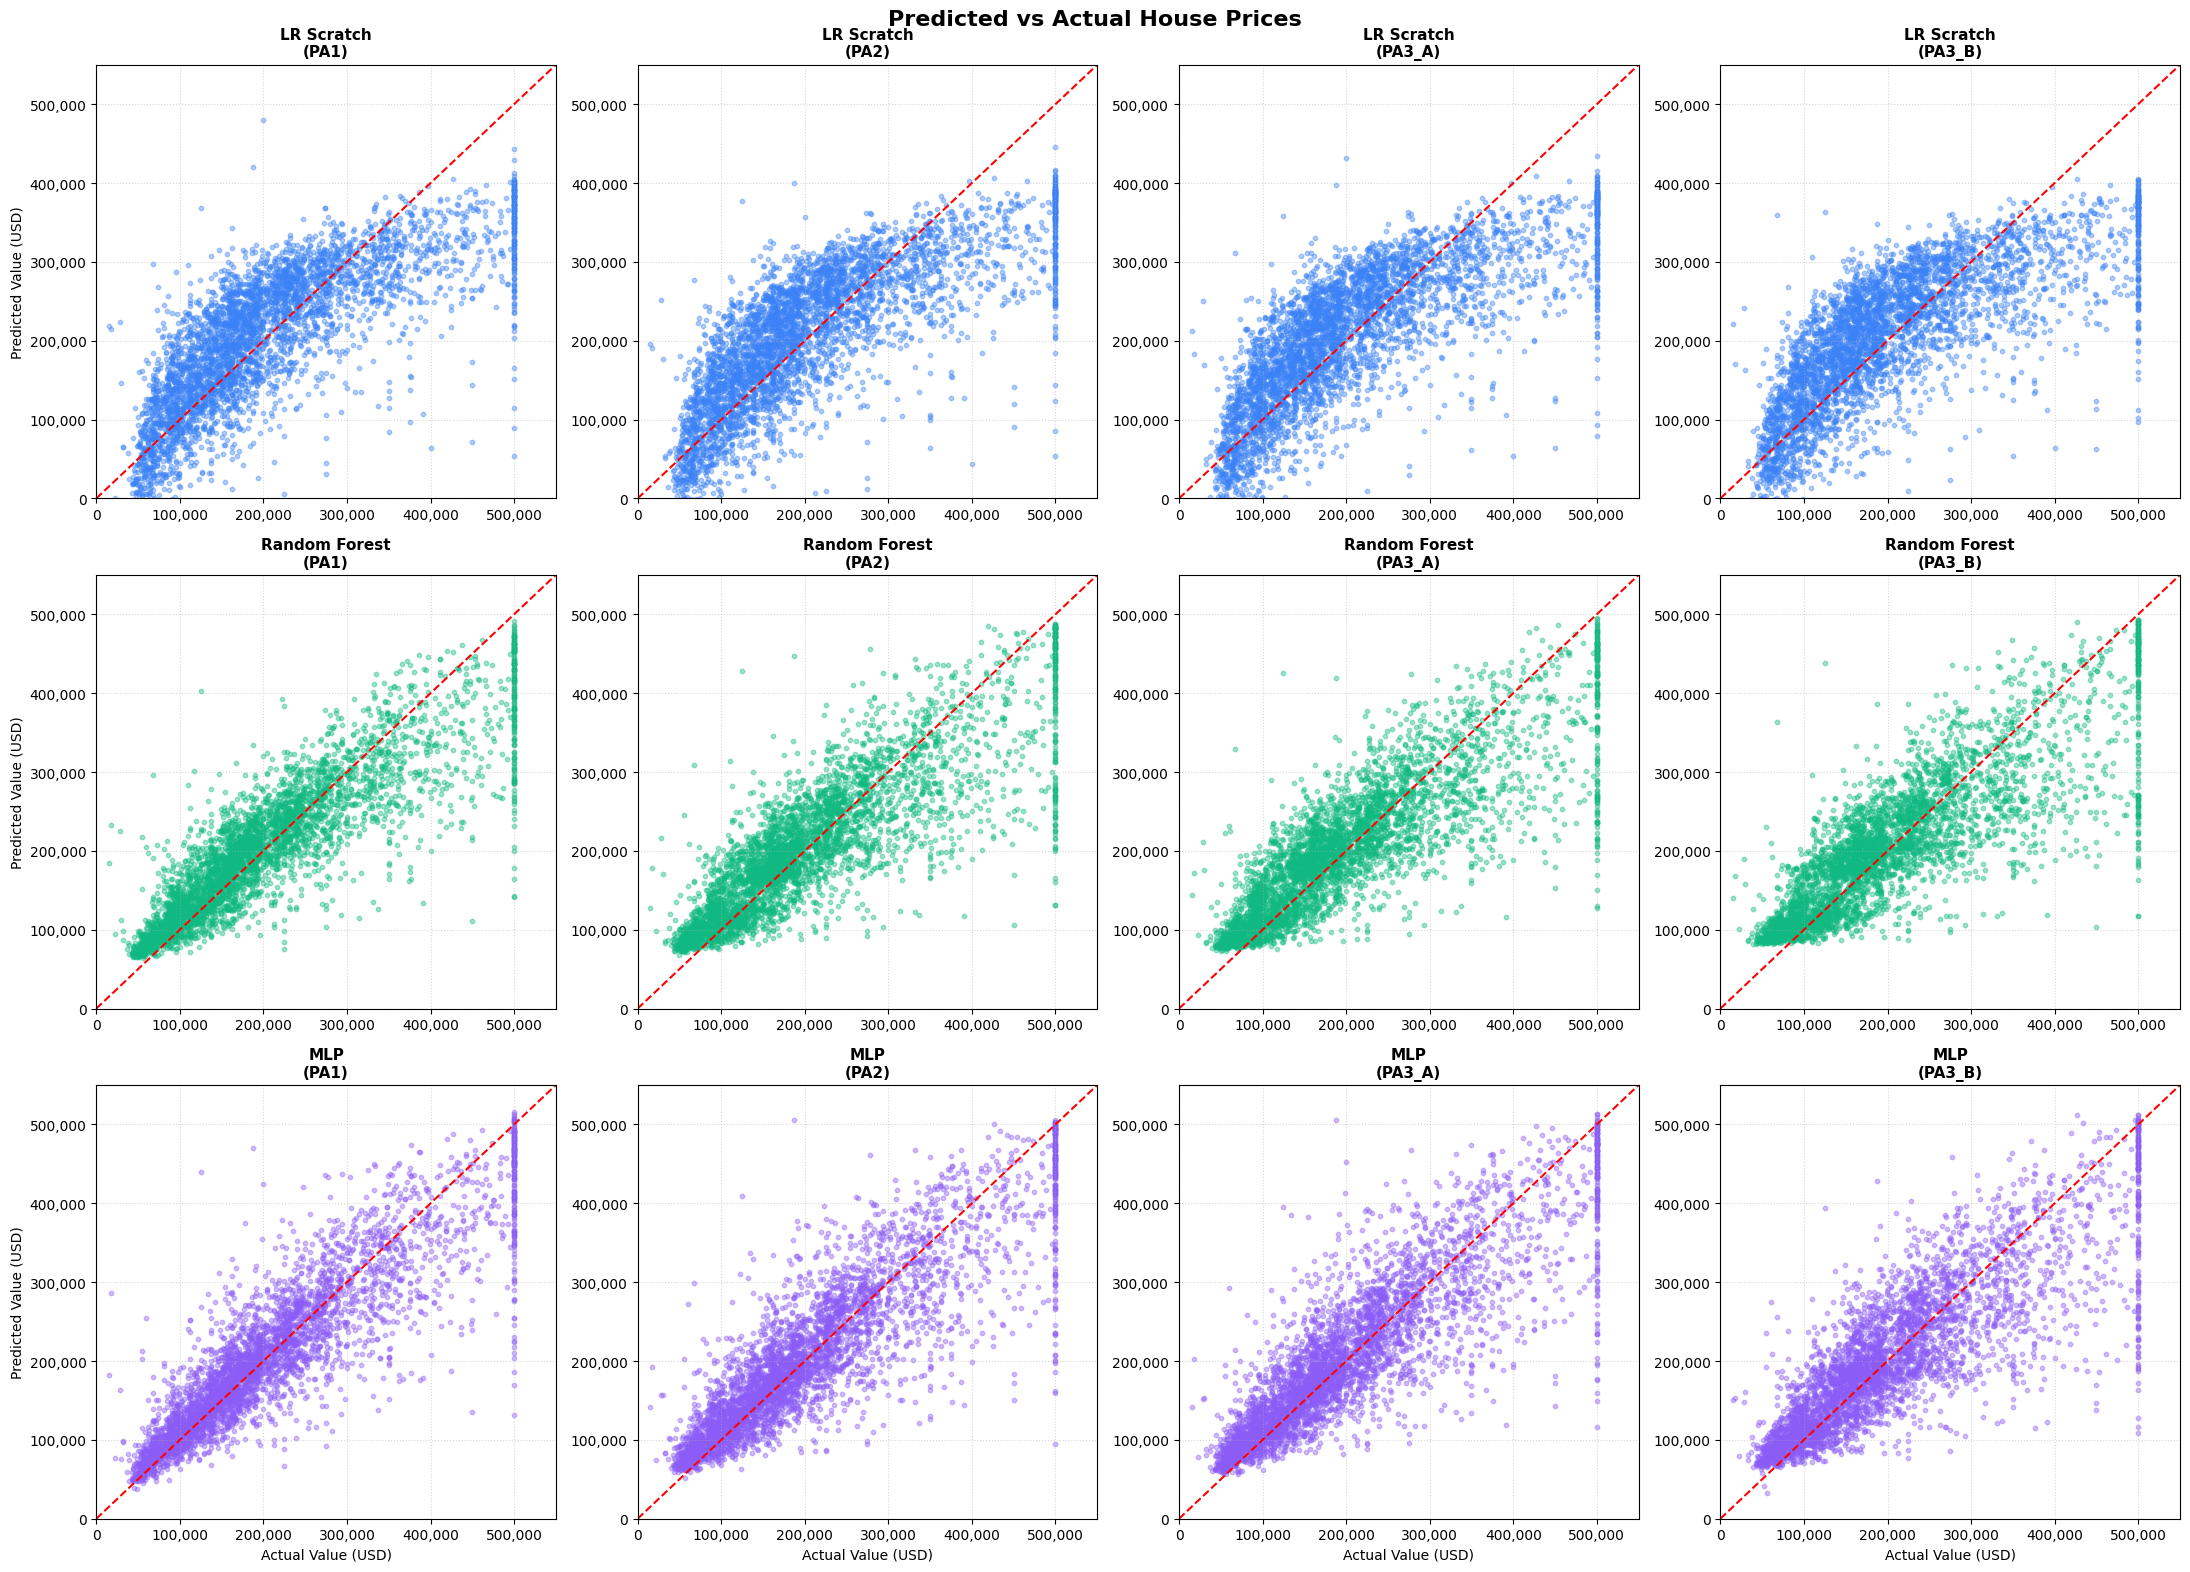
\includegraphics[width=0.95\textwidth]{figures/lab4_modeling_fig3.png}
    \caption{Predicted vs. Actual house price scatter plots (12-panel grid comparing all models and scenarios).}
    \label{fig:lab4_mod_3}
\end{figure}
Figure~\ref{fig:lab4_mod_3} displays the 12-panel Predicted vs. Actual scatter plots. The MLP plots under PA1 (top-left) show a tight clustering of points along the 45-degree diagonal line, confirming high prediction accuracy across the entire price range.

% ==========================================
% SECTION 5: REPOSITORY LINK
% ==========================================
\newpage
\section*{Code Repository and Source Code Access}
All source code, Jupyter Notebooks, datasets, and execution logs compiled during the implementation of Lab 1, Lab 2, Lab 3, and Lab 4 are hosted in a public GitHub repository. 

The complete codebase can be accessed at the following URL: \\
\url{https://github.com/lacthui06/Lab-ML}

\end{document}
